\documentclass[a4paper, 9pt]{scrartcl}\usepackage[]{graphicx}\usepackage[]{xcolor}
% maxwidth is the original width if it is less than linewidth
% otherwise use linewidth (to make sure the graphics do not exceed the margin)
\makeatletter
\def\maxwidth{ %
  \ifdim\Gin@nat@width>\linewidth
    \linewidth
  \else
    \Gin@nat@width
  \fi
}
\makeatother

\definecolor{fgcolor}{rgb}{0.345, 0.345, 0.345}
\newcommand{\hlnum}[1]{\textcolor[rgb]{0.686,0.059,0.569}{#1}}%
\newcommand{\hlstr}[1]{\textcolor[rgb]{0.192,0.494,0.8}{#1}}%
\newcommand{\hlcom}[1]{\textcolor[rgb]{0.678,0.584,0.686}{\textit{#1}}}%
\newcommand{\hlopt}[1]{\textcolor[rgb]{0,0,0}{#1}}%
\newcommand{\hlstd}[1]{\textcolor[rgb]{0.345,0.345,0.345}{#1}}%
\newcommand{\hlkwa}[1]{\textcolor[rgb]{0.161,0.373,0.58}{\textbf{#1}}}%
\newcommand{\hlkwb}[1]{\textcolor[rgb]{0.69,0.353,0.396}{#1}}%
\newcommand{\hlkwc}[1]{\textcolor[rgb]{0.333,0.667,0.333}{#1}}%
\newcommand{\hlkwd}[1]{\textcolor[rgb]{0.737,0.353,0.396}{\textbf{#1}}}%
\let\hlipl\hlkwb

\usepackage{framed}
\makeatletter
\newenvironment{kframe}{%
 \def\at@end@of@kframe{}%
 \ifinner\ifhmode%
  \def\at@end@of@kframe{\end{minipage}}%
  \begin{minipage}{\columnwidth}%
 \fi\fi%
 \def\FrameCommand##1{\hskip\@totalleftmargin \hskip-\fboxsep
 \colorbox{shadecolor}{##1}\hskip-\fboxsep
     % There is no \\@totalrightmargin, so:
     \hskip-\linewidth \hskip-\@totalleftmargin \hskip\columnwidth}%
 \MakeFramed {\advance\hsize-\width
   \@totalleftmargin\z@ \linewidth\hsize
   \@setminipage}}%
 {\par\unskip\endMakeFramed%
 \at@end@of@kframe}
\makeatother

\definecolor{shadecolor}{rgb}{.97, .97, .97}
\definecolor{messagecolor}{rgb}{0, 0, 0}
\definecolor{warningcolor}{rgb}{1, 0, 1}
\definecolor{errorcolor}{rgb}{1, 0, 0}
\newenvironment{knitrout}{}{} % an empty environment to be redefined in TeX

\usepackage{alltt}
\usepackage[ngerman]{babel}

% -----------------------------------------------------------------------

% -----------------------------------------------------------------------
%% ------------------------------------------------------------
%% by J.Kruppa on Friday, February 11, 2022 (11:31)
%% \def\mainDir{\Sexpr{exam_path}}
\def\source{/Users/jokruppa/source/tex}
\usepackage[margin=2cm, includefoot]{geometry}
\setlength{\parindent}{0cm}
\usepackage{booktabs}
\usepackage{amsmath}
\usepackage{scalerel,amssymb}
\usepackage{setspace}
\def\csquare{{\Large $\boxtimes$}}
\def\msquare{{\Large $\square$}}
\usepackage[normalem]{ulem}
\usepackage{array}
\usepackage{xcolor}
\usepackage{float}
\usepackage{currfile}
\usepackage{tikz}
\usepackage[nomessages]{fp}

%% beamer defs
\def\lecture{Klausurfragen der Bio Data Science}

%% exam defs
\def\examtitle{\lecture}
\def\exammodule{
\vspace{-1.75cm}  
\begin{graybox}{}
\vspace{2Ex}
\textbf{\large Name:} \rule[0ex]{16.75em}{.4pt}
\hfill \textnormal{\textit{Nicht bestanden:}} \msquare \\[2.5Ex]
\textbf{\large Vorname:} \rule[0ex]{15em}{.4pt} \\[2.5Ex]
\textbf{\large Matrikelnummer:} \rule[0ex]{10.8em}{.4pt}
\hfill Endnote: \rule[0ex]{7em}{.4pt} 
\end{graybox}
\vspace{3Ex}
\phantom{text}
}
\def\examsemester{Sommersemester \& Wintersemester}
\def\examdate{\today}
%% ------------------------------------------------------------
\definecolor{darkblue}{rgb}{0,0,.5}
\definecolor{darkpurple}{rgb}{0.4117, 0.2, 0.4117}
\definecolor{uni}{rgb}{0,0.3137,0.6078}
\definecolor{gray}{gray}{0.7}

\usepackage{tcolorbox}
\definecolor{logo1}{RGB}{0, 158, 227}
\definecolor{gray5}{RGB}{247, 247, 247}
\definecolor{gray2}{RGB}{102, 102, 102}

\newtcolorbox{graybox}[1]{
  colback=gray5,%%red!5!white,
  colframe=gray2,%%red!75!black,
  fonttitle=\bfseries\Large,
  %%valign=center,
  fontupper=\large,
  before skip=10pt plus 2pt,
  after skip=20pt plus 4pt,
  title=#1}

\newtcolorbox{takehomebox}[1]{
  colback=gray5,%%red!5!white,
  colframe=logo1,%%red!75!black,
  fonttitle=\bfseries\Large,
  %%valign=center,
  fontupper=\large,
  before skip=10pt plus 2pt,
  after skip=10pt plus 2pt,
  title=#1}

\def\Rlogo{
\includegraphics[width = 0.5cm]{\string~/Documents/GitHub/exam/img/Rlogo}\;}

\usepackage[scaled=.90]{helvet} 
\usepackage{fancyhdr}
\usepackage{lastpage}
\usepackage{hyperref}
\hypersetup{
    colorlinks=true,       % false: boxed links; true: colored links
    linkcolor=black,          % color of internal links 
    urlcolor=magenta           % color of external links
}
\renewcommand{\familydefault}{\sfdefault}

\title{
\large \exammodule \\[5Ex]
\Huge \examtitle \\[2Ex] 
\Large Hochschule Osnabr{\"u}ck
}
\author{Pr{\"u}fer: Prof. Dr. Jochen Kruppa \\
Fakult{\"a}t f{\"u}r Agrarwissenschaften und Landschaftsarchitektur \\ 
j.kruppa@hs-osnabrueck.de}
\date{Version vom \examdate}

%% ------------------------------------------------------------
%% by J.Kruppa on Tuesday, September 23, 2014 (12:50)
%% Header
\renewcommand{\headrulewidth}{0pt}
\renewcommand{\footrulewidth}{0pt}
\pagestyle{fancy}

\fancyhf{}
\fancyhead[L]{}
\fancyhead[R]{}
\fancyfoot[R]{\thepage}
\fancyfoot[L]{\footnotesize \examtitle}

\fancypagestyle{empty}{
 \fancyhf{}
 \fancyhead[L]{}
 \fancyhead[R]{}
 \fancyfoot[R]{\thepage}
 \fancyfoot[L]{\footnotesize \examtitle}
}

\usepackage{arevtext,arevmath}

\newcommand\Tstrut{\rule{0pt}{2.6ex}}         % = `top' strut
\newcommand\Bstrut{\rule[-0.9ex]{0pt}{0pt}}   % = `bottom' strut
\def\strut{\Tstrut\Bstrut}

% -----------------------------------------------------------------------
\IfFileExists{upquote.sty}{\usepackage{upquote}}{}
\begin{document}
\date{Wintersemester 2024/25 
\vfill
\begin{center}

\includegraphics[width = 1.9cm]{avatare/Alex}\hspace{-8mm}

\includegraphics[width = 1.9cm]{avatare/Jessica}\hspace{-8mm}

\includegraphics[width = 1.9cm]{avatare/Jonas}\hspace{-8mm}

\includegraphics[width = 1.9cm]{avatare/Mark}\hspace{-8mm}

\includegraphics[width = 1.9cm]{avatare/Nilufar}\hspace{-8mm}

\includegraphics[width = 1.9cm]{avatare/Paula}\hspace{-8mm}

\includegraphics[width = 1.9cm]{avatare/Steffen}\hspace{-8mm}

\includegraphics[width = 1.9cm]{avatare/Tina}\hspace{-8mm}

\includegraphics[width = 1.9cm]{avatare/Yuki}\\
\small
\vspace{1.5Ex}
\textit{"`The test of a student is not how much he knows,\\ but how much he wants to know."'\\ --- Alice W. Rollins}
\end{center}}
% -----------------------------------------------------------------------
\maketitle
\fancypagestyle{empty}{
  \fancyfoot[L]{\tiny $\blacksquare\!\blacksquare\!\blacksquare\!\square\!\blacksquare\!\square\!\blacksquare\!\blacksquare\!\square\!\blacksquare\!\blacksquare\!\blacksquare\!\blacksquare\!\square\!\square\!\blacksquare\!\blacksquare\!\square\!\blacksquare\!\square$}
}
\thispagestyle{empty}
\clearpage
% -----------------------------------------------------------------------
\begin{minipage}[c]{0.125\textwidth}

\includegraphics[width = 1.9cm]{avatare/Alex}
\end{minipage}
\begin{minipage}[c]{0.875\textwidth}
\textit{Alex studiert im 3. Semester und wiederholt das Modul, da er im ersten Jahr andere Prioritäten für sich gesetzt hat. Das musste sein, da er sich ziemlich im Abitur verausgabt hat. Darüber hinaus war die WG auch eher auf Party angelegt. Alex hofft jetzt über Pünktlichkeit wieder in die Bahn zu kommen. Dafür steht er jetzt immer um 5 Uhr auf! Freunde von ihm beschreiben ihn eher als extrovertiert. Er kennt Paula noch aus der Schulzeit und er überlegt, ob nicht beide Mal nach Mallorca sollten.} 
\end{minipage}\\[2.75Ex]
% -----------------------------------------------------------------------
\begin{minipage}[c]{0.875\textwidth}
\textit{Nach zwei Semestern Studium an der Universität Osnabrück war es dann Jessica doch viel zu theoretisch. Etwas angewandtes sollte es sein, wo sie auch eine Fähigkeit lernt, die frau nutzen kann. Deshalb hat sich Jessica an der Hochschule eingeschrieben. Hoffentlich lernt sie etwas nützliches, wo andere für Geld geben würden. Wer nützlich ist, ist wertvoll. Ihr Traum ist ja eine Hundeschule aufzumachen. Die großen Parties hat sie immer gemieden. Sie ist lieber mit ihrer Hündin im Teuteburgerwald.}
\end{minipage}
\begin{minipage}[c]{0.125\textwidth}

\includegraphics[width = 1.9cm]{avatare/Jessica}
\end{minipage}\\[2.75Ex]
% -----------------------------------------------------------------------
\begin{minipage}[c]{0.125\textwidth}

\includegraphics[width = 1.9cm]{avatare/Jonas}
\end{minipage}
\begin{minipage}[c]{0.875\textwidth}
\textit{Das ist jetzt der letzte Versuch mit einem Studium. Wenn es nicht klappt dann überlegt Jonas das \href{https://www.ihk.de/osnabrueck/aus-und-weiterbildung/ausbildung/ausbildungsbetriebe/projekt-neustart-1087206}{Programm der IHK zu Ausbildungsvermittlung} zu nutzen. Aber eine Runde gibt er sich noch. Struktur ist eigentlich das Wichtigste und diesmal hat er sich alle Altklausuren der Fachschaft besorgt. Dann ist er auch noch gleich der Fachschaft beigetreten um mehr Informationen abzugreifen. Und er versucht nicht seine Zeit mit Alex zu verdaddeln oder in der Fachschaft bei einem Bier oder so...}
\end{minipage}\\[2.75Ex]
% -----------------------------------------------------------------------
\begin{minipage}[c]{0.875\textwidth}
\textit{Nächstes Semester geht es nach Kanada davon hat er schon auf der Berufsschule geträumt. Deshalb konzentriert er sich sehr auf die Prüfungen. Ein Schiff ist im Hafen sicher, aber dafür ist es nicht gebaut worden. Das \href{https://www.hs-osnabrueck.de/wir/fakultaeten/aul/international/}{International Faculty Office} der Fakultät Agrarwissenschaften und Landschaftsarchitektur hat super geholfen, aber es waren einiges an Unterlagen. Jetzt hofft er, dass Tina dann doch noch mitkommt. Aber sonst macht er das eben alleine. Obwohl das eher nicht so seine Art ist. Vielleicht sollte er sich mal einen Tipp bei Tina holen, sie wirkt sehr entschlossen.} 
\end{minipage}
\begin{minipage}[c]{0.125\textwidth}

\includegraphics[width = 1.9cm]{avatare/Mark}
\end{minipage}\\[2.75Ex]
% -----------------------------------------------------------------------
\begin{minipage}[c]{0.125\textwidth}

\includegraphics[width = 1.9cm]{avatare/Nilufar}
\end{minipage}
\begin{minipage}[c]{0.875\textwidth}
\textit{Nach der Ausbildung wollte Nilufar eigentlich gleich anfangen zu arbeiten, aber nach einem Praktikum und der Probezeit stellte sie fest, dass es ohne einen Hochschulabschluss schwer wird Führungsverantwortung zu übernehmen. Mit Menschen kann sie schon immer und dann auch eigene Projekte mit anderen verwirklichen, dass ist doch was. Mit dem notwendigen Abschluss sollte der Start um so einfacher sein. Dann ist sie keine Befehlsempfängerin mehr sondern gibt die Marschrichtung vor. Schon jetzt koordiniert Nilufar das Studium von anderen.}
\end{minipage}\\[2.75Ex]
% -----------------------------------------------------------------------
\begin{minipage}[c]{0.875\textwidth}
\textit{Paula möchte die Welt zu einem besseren Ort machen. Wenn da nicht die anderen Mitmenschen wären. Paula muss das Modul nochmal wiederholen, da es dann am Ende des Semesters zu viel für sie wurde. Eine Lerngruppe hätte geholfen, aber das ist dann gar nicht so einfach eine zu finden. Zwar kennt sie schon Nilufar, aber Nilufar ist ihr manchmal zu forsch. Ihr schwant aber, dass alleine das Studium sehr schwer werden wird. Das Abitur war schon so ein Lernhorror, das möchte sie nicht nochmal. Alex sieht sie da als Vorbild.}
\end{minipage}
\begin{minipage}[c]{0.125\textwidth}

\includegraphics[width = 1.9cm]{avatare/Paula}
\end{minipage}\\[2.75Ex]
% -----------------------------------------------------------------------
\begin{minipage}[c]{0.125\textwidth}

\includegraphics[width = 1.9cm]{avatare/Steffen}
\end{minipage}
\begin{minipage}[c]{0.875\textwidth}
\textit{Sommer, Sonne, Natur. Das ist es was Steffen mag. Raus in die Komune und die Natur genießen. Leider hat Steffen noch andere Bedürfnisse, die ein Einkommen benötigen. Da Studierte mehr verdienen, würde dann in Teilzeit auch mehr rausspringen. Wenn er dann privat was anbauen kann, dann spart er gleich doppelt. Leider sind viele seiner Kommilitonen total verkrampfte Karrieristen. Es geht nur ums Äußere. Dabei verliert sich Steffen gerne im Prozess. Das hat auch seinen Schulabschluss etwas verzögert. Steffen lässt sich eben Zeit.}
\end{minipage}\\[2.75Ex]
% -----------------------------------------------------------------------
\begin{minipage}[c]{0.875\textwidth}
\textit{Wille  war es, die es Tina hierher gebracht hat und Wille wird es sein, die Tina dann auch zum Abschluß treibt. Nach einem Rückschlag muss Tina jetzt einige Module wiederholen, damit sie dann auch fertig wird. Ab und zu ist sie schwach gewesen und das hat dann Zeit gekostet. Das Tina es dann manchmal übertreibt, weiß sie nur zu gut, aber irgendwie muss die Kontrolle ja erhalten bleiben? Insbesondere, wenn sie mal wieder die Nacht durchgefeiert hat, verachtet Tina sich. Dann baut Nilufar sie dann bei einem Tee wieder auf.}
\end{minipage}
\begin{minipage}[c]{0.125\textwidth}

\includegraphics[width = 1.9cm]{avatare/Tina}
\end{minipage}\\[2.75Ex]
% -----------------------------------------------------------------------
\begin{minipage}[c]{0.125\textwidth}

\includegraphics[width = 1.9cm]{avatare/Yuki}
\end{minipage}
\begin{minipage}[c]{0.875\textwidth}
\textit{Für Yuki war es nicht einfach. Teilweise war die Krankheit sehr hinderlich, dann war es Yuki selber. Dann muss man auch wieder auf die Beine kommen und es dauert eben seine Zeit. Aber immerhin hat Yuki es jetzt den Abschluss gekriegt und hat einen Studienplatz. Jetzt heißt es in den Rhythmus kommen und schauen, was noch so passiert. Immerhin hat Yuki schon eine kleine Gruppe gefunden, in der Yuki dann Hilfe findet. Ist aber auch sehr unübersichtlich so ein Studium. Steffen ist immer super entspannt.}
\end{minipage}
\clearpage
% -----------------------------------------------------------------------


\begin{graybox}{Erlaubte Hilfsmittel}
  \vspace{1Ex}
  \begin{itemize}
  \item Normaler Taschenrechner ohne Möglichkeit der Kommunikation mit anderen
    Geräten! Ausdrücklich kein Handy!
  \item Eine DIN A4-Seite als beidseitig, selbstgeschriebene,
    handschriftliche Formelsammlung. Keine digitalen Ausdrucke! 
  \item \textbf{\textcolor{red}{Die Verwendung eines roten Farbstiftes ist nicht gestattet! Korrekturfarbe!}}
  \item \textit{You can answer the questions in English without any consequences.}  
  \end{itemize}
\end{graybox}
\vfill

\begin{graybox}{Endnote}
  \vspace{1Ex}
  \begin{itemize}
  \item[] \rule[0ex]{3em}{.4pt}\, von 20\, Punkten sind aus den Multiple
    Choice Aufgaben erreicht.
  \item[] \rule[0ex]{3em}{.4pt}\, von 72 Punkten sind aus den Rechen- und
    Textaufgaben erreicht. 
  \item[] \rule[0ex]{3em}{.4pt}\, von 92 Punkten in Summe.
  \item[] Es wird folgender Notenschlüssel angewendet.   
  \end{itemize}
  \vspace{1ex}
\begin{center}
  \begin{tabular}[c]{cc}
    \toprule
    \textbf{Punkte}	&	\textbf{Note}	\\
    \midrule
    88.0 - 92.0	&	1,0	\\
    83.5 - 87.5	&	1,3	\\
    78.5 - 83.0	&	1,7	\\
    74.0 - 78.0	&	2,0	\\
    69.5 - 73.5	&	2,3	\\
    65.0 - 69.0	&	2,7	\\
    60.5 - 64.5	&	3,0	\\
    55.5 - 60.0	&	3,3	\\
    51.0 - 55.0	&	3,7	\\
    46.0 - 50.5	&	4,0	\\
    \bottomrule
  \end{tabular}
\end{center}
  \vspace{1ex}
\begin{itemize}
\item[] Es ergibt sich eine Endnote von \rule[0ex]{4em}{.4pt}.
\end{itemize}
  \vspace{1Ex}
\end{graybox}

% -----------------------------------------------------------------------
\newpage
% -----------------------------------------------------------------------

\begin{graybox}{Multiple Choice Aufgaben}
  \begin{itemize}
  \item Pro Multipe Choice Frage ist \emph{genau} eine Antwort richtig.
  \item \textbf{Übertragen Sie Ihre Kreuze in die Tabelle auf
      dieser Seite.}
  \end{itemize}

\begin{center}
  \large
  \begin{tabular}{|l|c|c|c|c|c?c|}
    \hline
    & \textbf{A} & \textbf{B} & \textbf{C} & \textbf{D} & \textbf{E} & $\boldsymbol{\checkmark}$\strut\\
    \hline
    \textbf{Aufgabe 1} &   &   &   &   &   & \strut\\
    \hline
    \textbf{Aufgabe 2} &   &   &   &   &   & \strut\\
    \hline
    \textbf{Aufgabe 3} &   &   &   &   &   & \strut\\
    \hline
    \textbf{Aufgabe 4} &   &   &   &   &   & \strut\\
    \hline
    \textbf{Aufgabe 5} &   &   &   &   &   & \strut\\
    \hline
    \textbf{Aufgabe 6} &   &   &   &   &   & \strut\\
    \hline
    \textbf{Aufgabe 7} &   &   &   &   &   & \strut\\
    \hline
    \textbf{Aufgabe 8} &   &   &   &   &   & \strut\\
    \hline
    \textbf{Aufgabe 9} &   &   &   &   &   & \strut\\
    \hline
    \textbf{Aufgabe 10} &   &   &   &   &   & \strut\\
    \hline
  \end{tabular}
\end{center}

\begin{itemize}
\item Es sind \rule[0ex]{2em}{.4pt}\, von 20 Punkten erreicht worden.
\end{itemize}
\end{graybox}

\vfill

\begin{graybox}{Rechen- und Textaufgaben}
  \begin{center}
    \large
    \begin{tabular}{|l|c|c|c|c|c|c|c|}
      \hline
      \textbf{Aufgabe} & \textbf{11} & \textbf{12} & \textbf{13} & \textbf{14} & \textbf{15} & \textbf{16} & \textbf{17} \strut\\
      \hline
      \textbf{Punkte} & 
      \hspace{1Ex}\Large\textcolor{gray!70}{8}\hspace{1Ex}  & 
      \hspace{1Ex}\Large\textcolor{gray!70}{10}\hspace{1Ex}  & 
      \hspace{1Ex}\Large\textcolor{gray!70}{12}\hspace{1Ex}  & 
      \hspace{1Ex}\Large\textcolor{gray!70}{10}\hspace{1Ex}  & 
      \hspace{1Ex}\Large\textcolor{gray!70}{10}\hspace{1Ex}  & 
      \hspace{1Ex}\Large\textcolor{gray!70}{10}\hspace{1Ex}  & 
      \hspace{1Ex}\Large\textcolor{gray!70}{12}\hspace{1Ex} \strut\\
      \hline
  \end{tabular}
\end{center}
\begin{itemize}
\item Es sind \rule[0ex]{2em}{.4pt}\, von 72 Punkten erreicht worden.
\end{itemize}
\end{graybox}

% -----------------------------------------------------------------------
\clearpage
% -----------------------------------------------------------------------
\begin{graybox}{Multiple Choice Aufgaben}
Die Multiple Choice Aufgaben \textcolor{red}{unterliegen dem Zufall}. Die Reihenfolge der Antworten ist zufällig. Die Fragen und Antworten sind semantisch zufällig und haben somit \textcolor{red}{verschiedene Textvarianten}. Insbesondere die reinen Textaufgaben haben verschiedene Textvarianten. Die Semeantik mag sich unterscheiden, die Inhalte sind aber gleich.
\end{graybox}
\section*{ANOVA}

\section{Aufgabe \hfill (2 Punkte)}





Sie führen einen Versuch mit einer Behandlung und drei Faktorleveln durch. Danach rechnen Sie eine einfaktorielle ANOVA und es ergibt sich ein $\eta^2 = 0.31$. Welche Aussage ist richtig?



\begin{enumerate}
\item [\textbf{A} \msquare] Das $\eta^2$ ist ein Wert f{"u}r die G{"u}te der ANOVA. Je kleiner desto besser. Ein $\eta^2$ von 0 bedeutet ein perfektes Modell mit keiner Abweichung. Die Varianz ist null.
\item [\textbf{B} \msquare] Die Berechnung von $\eta^2$ ist ein Wert f{"u}r die Interaktion.
\item [\textbf{C} \msquare] Das $\eta^2$ ist die Korrelation der ANOVA. Mit der Ausnahme, dass 0 der beste Wert ist.
\item [\textbf{D} \msquare] Das $\eta^2$ wird genutzt um zu erfahren welchen Anteil der Varianz die Behandlungsbedingungen erklären.
\item [\textbf{E} \msquare] Das $\eta^2$ beschreibt den Anteil der Varianz, der von den Behandlungsbedingungen nicht erkl{"a}rt wird. Somit der Rest an nicht erkl{"a}rbarer Varianz.
\end{enumerate} 

\section{Aufgabe \hfill (2 Punkte)}



Sie führen ein Feldexperiment durch um das Gewicht von Kartoffel zu
steigern. Die Pflanzen wachsen unter einer Kontrolle und zwei verschiedenen
Behandlungsbedingungen. Nach der Berechnung einer einfaktoriellen ANOVA
ergibt sich ein $\eta^2 = 0.2$. Welche Aussage ist richtig?



\begin{enumerate}
\item [\textbf{A} \msquare] Mit dem $\eta^2$ lässt sich auf die Qualität der Randomisierung und damit der Strukturgleichheit zwischen der Grundgesamtheit und der Stichprobe schließen. Es gilt dabei die Regel, dass ein $\eta^2$-Wert von 1 zu bevorzugen ist.
\item [\textbf{B} \msquare] Es werden 80\% der Varianz durch die Behandlung erklärt. Das $\eta^2$ beschreibt den Anteil der Varianz, der von den unterschiedlichen Behandlungsbedingungen nicht erklärt wird.
\item [\textbf{C} \msquare] Es werden 20\% der Varianz durch den Versuch erklärt. Das $\eta^2$ beschreibt den Anteil der Varianz, der durch Fehler in der Versuchsdurchführung entsteht.
\item [\textbf{D} \msquare] Es werden 20\% der Varianz durch die Behandlung erklärt. Das $\eta^2$ beschreibt den Anteil der Varianz, der von den unterschiedlichen Behandlungsbedingungen erklärt wird.
\item [\textbf{E} \msquare] Das $\eta^2$ beschreibt den Anteil der Varianz, der von den Umweltbedingungen erklärt wird. Daher werden 20\% der Varianz durch die Umweltbedingungen erklärt. Der Anteil der Varianz durch die Behandlungsgruppen ist dann 80\%.
\end{enumerate} 

\section{Aufgabe \hfill (2 Punkte)}



Sie rechnen eine einfaktorielle ANOVA und erhalten eine Teststatistik. Nun müssen Sie diese Teststatistik interpretieren. Welche Aussage ist richtig?



\begin{enumerate}
\item [\textbf{A} \msquare] Wenn die F-Statistik kleiner als der kritische Wert ist kann die Nullhypothese nicht abgelehnt werden. Die F-Statistik ist der Quotient der MS der Behandlung durch die MS des Fehlers.
\item [\textbf{B} \msquare] Die ANOVA berechnet die F-Statistik indem die MS des Fehlers durch die MS der Behandlung geteilt werden. Wenn die F-Statistik sich der 1 ann{"a}hert kann die Nullhypothese nicht abgelehnt werden.
\item [\textbf{C} \msquare] Die ANOVA berechnet die T-Statistik aus der Multiplikation der MS Behandlung mit der MS der Fehler. Wenn die F-Statistik genau 0 ist, kann die Nullhypothese nicht abgelehnt werden.
\item [\textbf{D} \msquare] Die ANOVA berechnet die T-Statistik indem den Mittelwertsunterschied der Gruppen simultan durch die Standardabweichung der Gruppen teilt. Wenn die T-Statistik h{"o}her als 1.96 ist, kann die Nullhypothese abgelehnt werden.
\item [\textbf{E} \msquare] Wenn die F-Statistik höher ist als der kritische Wert kann die Nullhypothese nicht abgelehnt werden. Die F-Statistik ist die Differenz der MS der Behandlung durch die MS des Fehlers.
\end{enumerate} 

\section{Aufgabe \hfill (2 Punkte)}




Die ANOVA ist ein statistisches Verfahren welches häufig in den Auswertungen von Experimenten in den Agrarwissenschaften angewendet
wird. Dabei wird die ANOVA als ein erstes statistischen Werkzeug für die
Übersicht über die Daten benutzt. Eine ANOVA testet dabei...



\begin{enumerate}
\item [\textbf{A} \msquare] ... den Unterschied zwischen der Varianz durch verschiedene Behandlungsguppen unter der Varianz über alle Behandlungsgruppen. Wenn die ANOVA signifikant ist, kann kein Effekt $\eta^2$ bestimmt werden.
\item [\textbf{B} \msquare] ... den Unterschied zwischen der Varianz ausgelöst durch alle Behandlungsgruppen und der Varianz aus globalen Behandlungsguppen der Kontrollen. Wenn die ANOVA nicht signifikant ist, muss ein Posthoc-Test ausgeschlossen werden.
\item [\textbf{C} \msquare] ... den Unterschied zwischen der Varianz über alle Behandlungsgruppen und der Varianz aus verschiedenen Behandlungsguppen. Wenn die ANOVA signifikant ist, muss ein Posthoc-Test angeschlossen werden.
\item [\textbf{D} \msquare] ... den Unterschied zwischen mehreren Varianzen aus verschiedenen Behandlungsguppen. Wenn die ANOVA signifikant ist, ist nicht bekannt welcher Vergleich konkret unterschiedlich ist.
\item [\textbf{E} \msquare] ... den Unterschied zwischen der Varianz in den verschiedenen Behandlungsguppen und der Varianz in einer der Behandlungsgruppen. Wenn die ANOVA signifikant ist, muss über einen Posthoc-Test nachgedacht werden um den signifikanten Unterschied in einer der Gruppen exakt zu bestimmen.
\end{enumerate} 

\section{Aufgabe \hfill (2 Punkte)}



Die folgende Abbildung enthält die Daten aus einer Studie zur Bewertung der Wirkung von Vitamin C auf das Zahnwachstum bei Schweine. Der Versuch wurde an 69 Tieren durchgeführt, wobei jedes Tier eine von  drei Vitamin-C-Dosen (0.5, 1 und 1.5 mg/Tag) über eine von zwei Verabreichungsmethoden erhielt. Welche Aussage ist richtig im Bezug auf eine zweifaktorielle ANOVA?



{\centering 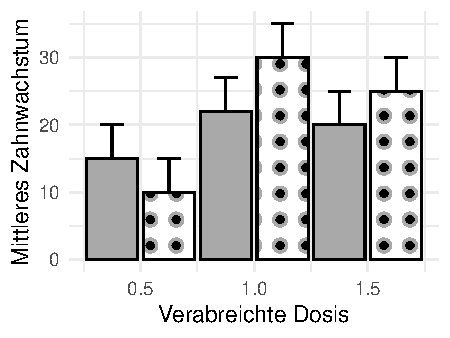
\includegraphics[width=\maxwidth]{img/mc-anova-02-a-1} 

}







\begin{enumerate}
\item [\textbf{A} \msquare] Eine Korrelation liegt vor $(p \leq 0.05)$.
\item [\textbf{B} \msquare] Das Bestimmtheitsmaß $R^2$ ist groß.
\item [\textbf{C} \msquare] Die Koeffizienten sind negativ $(\beta_0 < 0; \beta_1 < 0)$.
\item [\textbf{D} \msquare] Eine mittlere bis starke Interaktion liegt vor $(p \leq 0.05)$
\item [\textbf{E} \msquare] Keine Interaktion liegt vor $(p \leq 0.05)$.
\end{enumerate} 
\section*{Deskriptive Statistik \& Explorative Datenanalyse}

\section{Aufgabe \hfill (2 Punkte)}




Berechnen Sie den Mittelwert und Standardabweichung von $y$ mit 10, 15, 7, 14 und 12.



\begin{enumerate}
\item [\textbf{A} \msquare] Sie erhalten 11.6 +/- 1.79
\item [\textbf{B} \msquare] Es berechnet sich 11.6 +/- 10.3
\item [\textbf{C} \msquare] Sie erhalten 11.6 +/- 3.21
\item [\textbf{D} \msquare] Es berechnet sich 12.6 +/- 10.3
\item [\textbf{E} \msquare] Sie erhalten 11.6 +/- 1.605
\end{enumerate} 

\section{Aufgabe \hfill (2 Punkte)}




Gegeben ist $y$ mit 5, 20, 12, 18, 14, 22 und 51. Berechnen Sie den Median, das $1^{st}$ Quartile sowie das $3^{rd}$ Quartile.




\begin{enumerate}
\item [\textbf{A} \msquare] Sie erhalten 18 +/- 22
\item [\textbf{B} \msquare] Sie erhalten 18 [10; 20]
\item [\textbf{C} \msquare] Es ergibt sich 20 +/- 12
\item [\textbf{D} \msquare] Es berechnet sich 19 [13; 21]
\item [\textbf{E} \msquare] Es ergibt sich 18 [12; 22]
\end{enumerate} 

\section{Aufgabe \hfill (2 Punkte)}



Die empfohlene Mindestanzahl an Beobachtungen für die Visualisierung mit einem Boxplot sind...



\begin{enumerate}
\item [\textbf{A} \msquare] Wir sollten zwei bis fünf Beobachtungen mindestens pro Gruppe vorliegen haben.
\item [\textbf{B} \msquare] 5 und mehr Beobachtungen.
\item [\textbf{C} \msquare] 10 Beobachtungen.
\item [\textbf{D} \msquare] Wir sollten eine Beobachtung mindestens pro Gruppe vorliegen haben.
\item [\textbf{E} \msquare] Damit wir hier sauber eine Abbilung von einem 
\end{enumerate}

\section{Aufgabe \hfill (2 Punkte)}



Sie wollen nach einem Feldversuch die Varianz berechnen. Welche der folgenden Rechenoperationen müssen durchgeführt werden?



\begin{enumerate}
\item [\textbf{A} \msquare] Wir berechnen erst den Mittelwert und dann die quadratischen Abstände zu dem Mittelwert. Diese quadratischen Abstände summieren wir auf und teilen am Ende durch die Fallzahl. Als letzten Schritt ziehen wir die quadratische Wurzel.
\item [\textbf{B} \msquare] Den Mittelwert berechen, dann die absoluten Abstände zum Mittelwert aufsummieren
\item [\textbf{C} \msquare] Als erstes berechnen wir den Mittelwert. Dann bilden wir die Summe der quadratischen Abstände zu dem Mittelwert. Abschließend subtrahieren wir die Fallzahl.
\item [\textbf{D} \msquare] Als erstes berechnen wir den Mittelwert. Dann bilden wir die Summe der quadratischen Abstände zu dem Mittelwert. Abschließend teilen wir durch die Fallzahl.
\item [\textbf{E} \msquare] Den Mittelwert berechnen und die Abstände quadrieren. Die Summe mit der Fallzahl multiplizieren.
\end{enumerate} 

\section{Aufgabe \hfill (2 Punkte)}



Nachdem Sie eine ANOVA und die paarweisen t-Tests über das \Rlogo Paket \{emmeans\} durchgeführt haben, müssen Sie Ihre Daten nochmal zur Überprüfung visualisieren. Sie entscheiden sich für den Boxplot. Welche statistischen Maßzahlen stellt der Boxplot dar?

 



\begin{enumerate}
\item [\textbf{A} \msquare] Den Mittelwert und die Varianz.
\item [\textbf{B} \msquare] Den Mittelwert und die Standardabweichung.
\item [\textbf{C} \msquare] Durch die Abbildung des Boxplot erhalten wir die Informationen über den Median und die Standardabweichung.
\item [\textbf{D} \msquare] Den Median und die Quartile.
\item [\textbf{E} \msquare] Der Boxplot stellt die Mittelwerte und die Varianz dar.
\end{enumerate}

\section{Aufgabe \hfill (2 Punkte)}



Nachdem Sie in einem Feldexperiment zu Leistungssteigerung von Kartoffel durchgeführt haben, berechnen Sie den Mittelwert und den Median. Der Mittelwert $\bar{y}$ und der Median $\tilde{y}$ unterscheiden sich. Welche Aussage ist richtig?



\begin{enumerate}
\item [\textbf{A} \msquare] Der Mittelwert und der Median sollten gleich sein, wenn keine Outlier in den Daten vorliegen. 
\item [\textbf{B} \msquare] Wenn sich der Mittelwert und der Median nicht unterscheiden, liegen vermutlich Outlier in den Daten vor.
\item [\textbf{C} \msquare] Wenn sich der Mittelwert und der Median unterscheiden, liegen vermutlich keine Outlier in den Daten vor.
\item [\textbf{D} \msquare] Der Mittelwert und der Median sollten sich unterscheiden sein, wenn Outlier in den Daten vorliegen. 
\item [\textbf{E} \msquare] Da sich der Mittelwert und der Median unterscheiden, ist der Datensatz nicht zu verwenden. Mittelwert und Median müssen gleich sein.
\end{enumerate}

\section{Aufgabe \hfill (2 Punkte)}



Sie wollen eine ANOVA im Anschluss an Ihr Feldexperiment rechnen. Dafür muss Ihr gemessener Endpunkt die Annahme einer Varianzhomogenität genügen. Zur Überprüfung können Sie folgende Visualisierung nutzen. Welche entsprechende Regel zur Abschätzung der Annahme einer Varianzhomogenität kommt zur Anwendung?



\begin{enumerate}
\item [\textbf{A} \msquare] In einer explorativen Datanalyse nutzen wir den Violinplot. Dabei sollte der Bauch am Rand liegen. Dann können wir von einer Varianzhomogenität ausgehen.
\item [\textbf{B} \msquare] Einen Barplot. Die Mittelwerte müssen alle auf einer Höhe liegen. Die Fehlerbalken haben hier keine Informationen.
\item [\textbf{C} \msquare] Wir erstellen uns für jede Behandlung einen Dotplot und schauen, ob die Dots und damit die Varianz für jede Behandlung gleich groß sind.
\item [\textbf{D} \msquare] Einen Boxplot. Der Median, dargestellt als Linie, muss in der Mitte des IQR, dargestellt durch die Box, liegen.
\item [\textbf{E} \msquare] Nach dem Einlesen der Daten nutzen wir einen Boxplot um zu schauen, ob alle Boxen über alle Behandlungen in etwa gleich groß sind. Damit ist dann auch das IQR in allen Behandlungen in etwa gleich.
\end{enumerate}

\section{Aufgabe \hfill (2 Punkte)}




In der Statistik müssen wir häufig überprüfen, ob unser Outcome einer bestimmten Verteilung folgt. Meistens überprüfen wir, ob eine
Normalverteilung vorliegt. Folgende drei Abbildungen eigenen sich im Besonderen für die Überprüfung einer Verteilungsannahme an eine Variable.





\begin{enumerate}
\item [\textbf{A} \msquare] Barplot, Mosaicplot, Violinplot
\item [\textbf{B} \msquare] Scatterplot, Mosaicplot, Boxplot
\item [\textbf{C} \msquare] Densityplot, Boxplot, Violinplot
\item [\textbf{D} \msquare] Scatterplot, Densityplot, Barplot
\item [\textbf{E} \msquare] Histogramm, Scatterplot, Boxplot
\end{enumerate} 

\section{Aufgabe \hfill (2 Punkte)}



In dem folgenden Histogramm von $n = 233$ Pflanzen ist welche Verteilung abgebildet?



{\centering 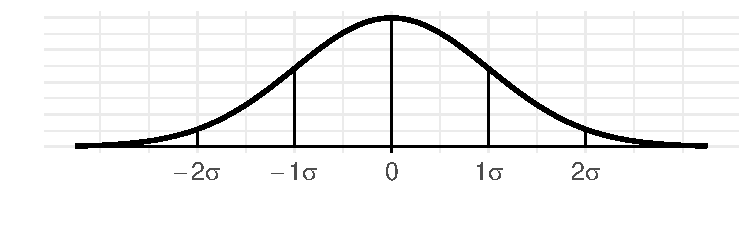
\includegraphics[width=\maxwidth]{img/mc-distribution-02-a-1} 

}







\begin{enumerate}
\item [\textbf{A} \msquare] In dem Histogramm ist eine Ordinalverteilung dargestellt.
\item [\textbf{B} \msquare] Es handelt sich um eine Binomial-Verteilung.
\item [\textbf{C} \msquare] Wir haben eine Gammaverteilung vorliegen.
\item [\textbf{D} \msquare] Dem Histogramm entnehmen wir eine Possion-Verteilung.
\item [\textbf{E} \msquare] In dem Histogramm ist eine Normalverteilung dargestellt.
\end{enumerate} 
\section*{Lineare Regression \& Korrelation}

\section{Aufgabe \hfill (2 Punkte)}



In Ihrer Abschlussarbeit wollen Sie ein prädiktives Modell rechnen. Jetzt stellt sich die Frage, was diese Entscheidung für Ihre Auswertung bedeutet. Welche Aussage ist richtig?



\begin{enumerate}
\item [\textbf{A} \msquare] Wenn ein prädiktives Modell gerechnet werden soll, dann muss zum einen ein Traingsdatensatz sowie ein Testdatensatz definiert werden. Dabei ist der Trainingsdatensatz meist 1/10 und der Testdatensatz 1/3 der Fallzahl groß. Der Testdatensatz dient zur Validierung.
\item [\textbf{B} \msquare] Es wird ein Trainingsdatensatz zum Trainieren des Modells benötigt. Der Testdatensatz dient zur Validierung. Dies gilt insbesondere für ein prädiktives Modell.
\item [\textbf{C} \msquare] Wenn ein prädiktives Modell gerechnet werden soll dann kann dies auf dem gesamten Datensatz geschehen. Das Ziel ist es einen Zusammenhang von $X$ auf $Y$ zu modellieren. Wie wirken sich die Einflussvariablen $Y$ auf die gemessenen Endpunkte $X = x_1, ..., x_p$ aus?
\item [\textbf{D} \msquare] Wenn ein prädiktives Modell gerechnet werden soll dann kann dies auf dem gesamten Datensatz geschehen. Das Ziel ist es einen Zusammenhang von $X$ auf $Y$ zu modellieren. Wie wirken sich die Einflussvariablen $X$ auf den gemessenen Endpunkt $Y$ aus?
\item [\textbf{E} \msquare] Es wird ein Trainingsdatensatz zum Modellieren des Trainingsmodells benötigt. Der Testdatensatz dient rein zur Visualisierung. Dies gilt vor allem für ein prädiktives Modell.
\end{enumerate}

\section{Aufgabe \hfill (2 Punkte)}



Nach einer Regressions sollten die Residuen normalverteilt sein. Was bei einer simplen Regression noch relativ einfach visuell in einem Scatterplot zu überprüfen ist. Für komplexere Modell liefert der QQ-Plot die notwendigen Informationen über die Normalverteilung. Welche Aussage ist richtig?



{\centering 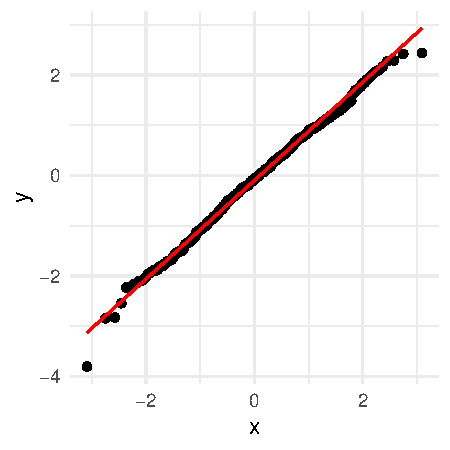
\includegraphics[width=\maxwidth]{img/mc-regression-05-a-1} 

}







\begin{enumerate}
\item [\textbf{A} \msquare] Wir betrachten insbesondere die beiden Enden der Gerade. Der Rest ist mehr oder minder egal, dann ist die Annahme an die Normalverteilung der Residuen erfüllt.
\item [\textbf{B} \msquare] Die Annahme der normalverteilten Residuen ist erfüllt. Die Punkte liegen zum überwiegenden Teil nicht auf der Geraden.
\item [\textbf{C} \msquare] Die Annahme der normalverteilten Residuen ist nicht erfüllt. Die Punkte liegen zum überwiegenden Teil nicht auf der Geraden.
\item [\textbf{D} \msquare] Wir betrachten die Gerade und dabei insbesondere die beiden Enden der Gerade in dem IQR, also dem ersten und dritten Quartile. Hier sollten die Punkte auf der Geraden liegen, dann ist die Annahme an die Normalverteilung der Residuen erfüllt.
\item [\textbf{E} \msquare] Die Annahme der normalverteilten Residuen ist nicht erfüllt. Die Punkte liegen zum überwiegenden Teil nicht auf der Geraden.
\end{enumerate}

\section{Aufgabe \hfill (2 Punkte)}



Nach der Modellierung einer Regression stellt sich die Frage, ob die Residuen (\texttt{.resid}) gleichmäßig um die gefitte Gerade liegen. Sie können folgende Abbildung für die visuelle Überprüfung der Residuen nutzen. Welche Aussage ist richtig?



{\centering 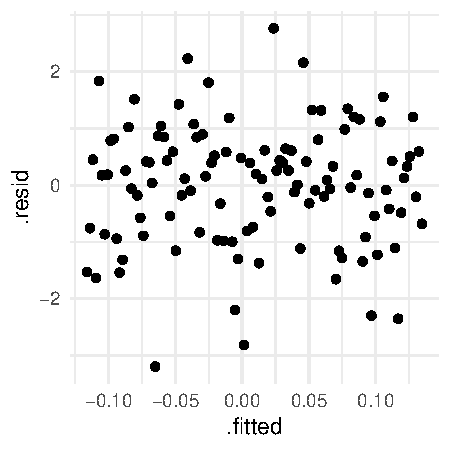
\includegraphics[width=\maxwidth]{img/mc-regression-06-a-1} 

}







\begin{enumerate}
\item [\textbf{A} \msquare] Die Annahme der normalverteilten Residuen ist erfüllt. Es ist ein Muster zu erkennen und wir können damit auf die Signifkanz von $x_1, ..., x_p$ schließen.
\item [\textbf{B} \msquare] Wir betrachten die Nulllinie und alle Punkte sollten ohne Muster gleichmäßig um die Nulllinie liegen. Da dies der Fal ist, gehen wir von keinen Ausreißern aus.
\item [\textbf{C} \msquare] Die Punkte müssen gleichmäßig, mit ähnlichen Abständen, in dem positiven wie auch negativen Bereich liegen. Dies ist hier klar nicht der Fall. Einzelne Ausreißer können beobachtet werden. Wir können mit dem Model so nicht rechnen und müssen erst die auffälligen Werte gesondert betrachten.
\item [\textbf{D} \msquare] Die Punkte müssen gleichmäßig in dem positiven Bereich liegen. Dies ist hier klar nicht der Fall. Einzelne Ausreißer können beobachtet werden. Die Analyse ist gescheitert.
\item [\textbf{E} \msquare] Die Annahme der normalverteilten Residuen ist nicht erfüllt. Es ist kein Muster zu erkennen.
\end{enumerate}

\section{Aufgabe \hfill (2 Punkte)}




Sie berechnen in Ihgrer Abschlussarbeit den Korrelationskoeffizienten $\rho$. Welche Aussage über den Korrelationskoeffizienten $\rho$ ist richtig?




\begin{enumerate}
\item [\textbf{A} \msquare] Der Korrelationskoeffizienten $\rho$ liegt zwischen -1 und 1. Darüber hinaus ist der Korrelationskoeffizienten $\rho$ einheitslos und kann als standardisierte Steigung verstanden werden.
\item [\textbf{B} \msquare] Korrelationskoeffizienten $\rho$ liegt zwischen 0 und 1. Darüber hinaus ist der Korrelationskoeffizienten $\rho$ einheitslos und kann als Standardisierung verstanden werden.
\item [\textbf{C} \msquare] Der Korrelationskoeffizienten $\rho$ liegt zwischen -1 und 1. Darüber hinaus ist der Korrelationskoeffizienten $\rho$ als standardisierte Steigung zu verstehen, wenn eine Standardisierung durchgeführt wurde. Diese Adjustierung nach Fischer muss am Anschluß der Berechnung der Korrelation durchgeführt werden.
\item [\textbf{D} \msquare] Der Korrelationskoeffizienten $\rho$ wird wie das $\eta^2$ aus der ANOVA interpretiert. Der Korrelationskoeffizienten $\rho$ beschreibt den Anteil an erklärter Varianz durch die Regression. Dabei gibt er jedoch eine Richtung an und kann auch negativ werden.
\item [\textbf{E} \msquare] Der Korrelationskoeffizienten $\rho$ zeigt keinen Zusammenhang zwischen zwei Variablen $x$ und $y$ bei einem Wert von 0. Einen negativen Zusammenhang Richtung -1 und somit auch einen positiven Zusammenhang Richtung 1. Je größer die Zahl allgemein, desto stärker der Effekt.
\end{enumerate}

\section{Aufgabe \hfill (2 Punkte)}



In einer lineren Regression kann es vorkommen, dass der Effekt repräsentiert durch den $\beta$ Koeffizienten nicht so richtig von der Größenordnung zu dem p-Wert passen will. So liefert eine Untersuchung des Einflusses von der $Fe_3O_4$-Konzentration in [$\mu g$] im Wasser auf den absoluten Proteingehalt in [$kg$] an Wasserlinsen folgende Effekte und p-Werte: $2e-04$ als p-Wert und einen $\beta_{Fe_3O_4}$ Koeffizienten von $1.1\times 10^{-5}$. Welche Aussage ist richtig?




\begin{enumerate}
\item [\textbf{A} \msquare] Wenn der Effekt $\beta_{Fe_3O_4}$ winzig ist, dann kann es an einer falsch gewählten Einheit liegen. Der Anstieg von einer Einheit in $X$ führt ja zu einer Änderung von $\beta_{Fe_3O_4}$ in $x$. Wir müssen daher die Einheit von $y$ entsprechend anpassen.
\item [\textbf{B} \msquare] Die Fallzahl ist zu klein angesetzt. Je kleiner die Fallzahl ist, desto höher ist die Teststatsitik und damit auch der $p$-Wert kleiner. Wir brauchen also mehr Fallzahl um den geringen Effekt noch signifikant zu krigen.
\item [\textbf{C} \msquare] Manchmal ist die Einheit der Einflussvariable $X$ zu groß gewählt, so dass der Ansteig von 1 Einheit in $X$ zu einer zu großen Änderung in $y$ führt. Daher kann der Effekt $\beta_{Fe_3O_4}$ sehr klein wirken, da der p-Wert wird auf einer einheitslosen Teststatistik bestimmt wird.
\item [\textbf{D} \msquare] Wenn der Effekt $\beta_{Fe_3O_4}$ sehr klein ist, dann kann es an einer falsch gewählten Einheit liegen. Der Anstieg von einer Einheit in $X$ führt ja zu einer Änderung von $\beta_{Fe_3O_4}$ in $y$. Daher ist hier mit einer anderen Einheit in den Daten zu rechnen, so dass wir hier einen besser formatierten Effekt sehen. Der p-Wert stammt aus einer einheitslosen Teststatistik.
\item [\textbf{E} \msquare] Die Fallzahl ist zu hoch angesetzt. Je höher die Fallzahl ist, desto kleiner ist die Teststatistik und damit ist dann auch der $p$-Wert sehr klein. Es sollte über eine Reduzierung der Fallzahl nachgedacht werden. Dann sollte der Effekt zum p-Wert passen.
\end{enumerate}

\section{Aufgabe \hfill (2 Punkte)}



Nachdem Sie Ihr Experiment abgeschlossen haben, stehen Sie vor der Frage wie Sie Ihre Daten modellieren sollen. In der Beispielauswertung von Ihrem Betreuenden finden Sie die Funktion \texttt{lm()} in \Rlogo. Welche Aussage ist richtig?





\begin{enumerate}
\item [\textbf{A} \msquare] Ist die Einflussvariable $X$ numerisch so werden die Gruppenmittelwerte geschätzt und eine anschließende ANOVA sowie multipler Gruppenvergleich mit \{emmeans\} ist möglich.
\item [\textbf{B} \msquare] Neben der klassichen Verwendung der Funktion \texttt{lm()} in der linearen Regression kann auch ein Gruppenvergleich gerechnet werden. Dafür müssen aber alle Faktoren aus den Daten entfernt und numerishc umgewandelt werden. Dann kann das R Paket \{emmeans\} genutzt werden um die Korrelation zu berechnen. Eine Adjustierung ist dann nicht mehr notwendig.
\item [\textbf{C} \msquare] Die Funktion \texttt{lm()} in \Rlogo ist der erste Schritt für einen Gruppenvergleich. Danach kann eine ANOVA oder aber ein multipler Vergleich in \{emmeans\} gerechnet werden. In der Funktion  \texttt{lm()} werden die Gruppenmittelwerte bestimmt.
\item [\textbf{D} \msquare] Die Funktion \texttt{lm()} in \Rlogo ist der letzte Schritt für einen Gruppenvergleich. Vorher kann eine ANOVA oder aber ein multipler Vergleich in \{emmeans\} gerechnet werden. In der Funktion  \texttt{lm()} werden die Gruppenvarianzen bestimmt.
\item [\textbf{E} \msquare] Die Funktion \texttt{lm()} berechnet die Varianzstruktur für eine ANOVA. Dannach kann dann über eine explorative Datenalayse nochmal eine Signifikanz berechnet werden. Sollte vor der Verwendung der Funktion \texttt{lm()} schon eine EDA gerechnet worden sein, so ist die Analyse wertlos.
\end{enumerate}

\section{Aufgabe \hfill (2 Punkte)}



In Ihrer Abschlussarbeit haben Sie neben den klassischen normalverteilten Endpunkte, wie Trockgewicht und Wuchshöhe noch den Infektionsstatus und Zähldaten erhoben. Um diese nicht normalverteilten Endpunkte auszuwerten nutzen Sie das \textit{generalisierte lineare Modell (GLM)}. Welche Aussage ist richtig?




\begin{enumerate}
\item [\textbf{A} \msquare] Das GLM ist ein faktisch maschineller Lernalgorithmus, der selstständig die Verteilungsfamilie für Y wählt.
\item [\textbf{B} \msquare] Das \textit{generalisierte lineare Modell (GLM)} erlaubt auch weitere Verteilungsgruppen für das $X$ bzw. die Einflussvariablen in einer linearen Regression zu wählen.
\item [\textbf{C} \msquare] Das GLM ist eine Vereinfachung des LM in R. Mit dem GLM lassen sich polygonale Regressionen rechnen. Somit stehen neben der Normalverteilung noch weitere Verteilungen zu Verfügung.
\item [\textbf{D} \msquare] Das GLM erlaubt auch nicht normalverteilte Residuen in der Schätzung der Regressionsgrade.
\item [\textbf{E} \msquare] Dank dem \textit{generalisierten linearen Modell (GLM)} können auch andere Verteilungsfamilien als die Normalverteilung mit einer linearen Regression modelliert werden.
\end{enumerate}
\section*{Vermischte Themen}  

\section{Aufgabe \hfill (2 Punkte)}

Die Randomisierung von Beobachtungen zu den Versuchseinheiten
ist bedeutend in der Versuchsplanung. Welche der folgenden Aussagen ist richtig?



\begin{enumerate}
\item [\textbf{A} \msquare] Durch eine Randomisierung können wir von Strukturgleichheit zwischen der Stichprobe und der Grundgesamtheit ausgehen.
\item [\textbf{B} \msquare] Randomisierung war bis 1952 bedeutend, wurde dann aber in Folge besserer Rechnerleistung nicht mehr verwendet. Aktuelle Statistik nutzt keine Randomisierung mehr.
\item [\textbf{C} \msquare] Strukturgleichheit ist durch Randomisierung gegeben. Leider hilft die Randomisierung noch nicht um von der Stichprobe auf die Grundgesamtheit zu schließen. Deshalb wurde das Falsifikationsprinzip entwickelt.
\item [\textbf{D} \msquare] Randomisierung erlaubt erst die Varianzen zu schätzen. Ohne eine Randomisierung ist die Berechnung von Mittelwerten und Varianzen nicht möglich. Dadurch lässt sich erst ein Experiment auswerten.
\item [\textbf{E} \msquare] Durch eine Randomisierung können wir nicht von Strukturgleichheit zwischen der Stichprobe und der Grundgesamtheit ausgehen.
\end{enumerate}

\section{Aufgabe \hfill (2 Punkte)}



Sie wollen Ihren Datensatz in \Rlogo einlesen und stehen nun vor einem Problem. Sie stellen fest, dass die Hilfeseiten alle in englischer Sprache verfasst sind. Warum mag die Nutzung von Deutsch problematisch sein?



\begin{enumerate}
\item [\textbf{A} \msquare] Es gibt keinen Grund nicht auch deutsche Wörter zu verwenden. Es ist ein Stilmittel.
\item [\textbf{B} \msquare] Programmiersprachen können nur englische Begriffe verarbeiten. Zusätzliche Pakete können zwar geladen werden, aber meist funktionieren diese Pakete nicht richtig. Deutsch ist International nicht bedeutend genug.
\item [\textbf{C} \msquare] Programmiersprachen haben Probleme mit Umlauten und Sonderzeichen der deutschen Sprache. Daher ist die Nutzung in Deutsch in den AGBs von \Rlogo untersagt.
\item [\textbf{D} \msquare] Die Spracherkennung von \Rlogo ist nicht in der Lage Deutsch zu verstehen.
\item [\textbf{E} \msquare] Im Allgemeinen haben Programmiersprachen Probleme mit Umlauten und Sonderzeichen, die in der deutschen Sprache vorkommen. Eine Nutzung der englischen Sprache umgeht dieses Problem auf einfache Art.
\end{enumerate}

\section{Aufgabe \hfill (2 Punkte)}



Bei der explorativen Datenanalyse (EDA) in \Rlogo gibt es eine richtige Abfolge von Prozessschritten, auch 	extit{Circle of life} genannt. Wie lautet die richtige Reihenfolge für die Erstellung einer EDA?



\begin{enumerate}
\item [\textbf{A} \msquare] Wir lesen als erstes die Daten über \texttt{read\_excel()} ein, transformieren die Spalten über \texttt{mutate()} in die richtige Form und können dann über \text{ggplot()} uns die Abbildungen erstellen lassen.
\item [\textbf{B} \msquare] Wir lesen die Daten über eine generische Funktion \texttt{read()} ein und müssen dann die Funktion \texttt{ggplot()} nur noch installieren. Dann haben wir die Abbildungen als \texttt{*.png} vorliegen.
\item [\textbf{C} \msquare] Für eine explorativen Datenanalyse (EDA) in \Rlogo müssen wir als erstes die Daten über \texttt{read\_excel()} einlesen. Danach müssen wir schauen, dass wir die Zeilen richtig über \texttt{mutate()} transformiert haben. Insbesondere müssen Variablen mit kontinuierlichen Werten in einen Faktor umgewandelt werden. Am Ende nutzen wir die Funktion \text{ggplot()} für die eigentlich EDA.
\item [\textbf{D} \msquare] Wir lesen die Daten ein und mutieren die Daten. Dabei ist wichtig, dass wir nicht das Paket \texttt{tidyverse} nutzen, da dieses Paket veraltet ist. über die Funktion \texttt{library(tidyverse)} entfernen wir das Paket von der Analyse.
\item [\textbf{E} \msquare] Die Funktionsreihenfolge ist wie folgt: \texttt{read\_excel()} ->  \texttt{mutate()} -> \text{ggplot()}. Dabei ist bei der Transformation der Daten darauf zu achten, dass keine Faktoren erstellt werden.
\end{enumerate}

\section{Aufgabe \hfill (2 Punkte)}



Es sei $s^2_1 = s^2_2$ in dem Modell $Y \sim X$. Welche Aussage ist richtig?



\begin{enumerate}
\item [\textbf{A} \msquare] Es handelt sich um ein unbalanciertes Design.
\item [\textbf{B} \msquare] Es liegt Varianzhomogenität vor.
\item [\textbf{C} \msquare] Es handelt sich um ein balanciertes Design.
\item [\textbf{D} \msquare] Es liegt Varianzhetrogenität vor.
\item [\textbf{E} \msquare] Es handelt sich um unabhängige Beobachtungen.
\end{enumerate}

\section{Aufgabe \hfill (2 Punkte)}



In einem Zuchtexperiment messen wir die Ferkel verschiedener Sauen. Die Ferkel einer Muttersau sind daher im statistischen Sinne...



\begin{enumerate}
\item [\textbf{A} \msquare] Die Ferkel stammen von der gleichen Sau und sind somit untereinander unabhängig.
\item [\textbf{B} \msquare] Die Ferkel stammen von der gleichen Sau und sind somit untereinander abhängig.
\item [\textbf{C} \msquare] Abhängig von der Stallanlage und des Experiments können die Ferkel abhängig oder unabhängig sein. Allgmein gilt, dass Ferkel von unterschiedlichen Sauen näher miteinander verwandt sind als Ferkel von gleichen Sauen. Das Fisher-Axiom.
\item [\textbf{D} \msquare] Je nach Stallanlage kommt eine andere Analyse in Betracht. Eine allgemeine Aussage über Ferkel und Sauen lässt sich statistisch nicht treffen.
\item [\textbf{E} \msquare] Untereinander unabhängig. Die Ferkel sind eigenständig und benötigen keine zusätzliche Behandlung.
\end{enumerate}

\section{Aufgabe \hfill (2 Punkte)}



Sie führen ein Experiment zur Behandlung von Klaueninfektionen bei Schweinen durch. Bei 3 Tieren finden Sie eine Erkrankung der Klauen vor und 7 Tiere sind gesund. Welche Aussage über den Effektschätzer Risk ratio ist richtig?



\begin{enumerate}
\item [\textbf{A} \msquare] Es ergibt sich ein Risk ratio von 2.33, da es sich um ein Anteil handelt.
\item [\textbf{B} \msquare] Der Anteil der Kranken wird berechnet. Da es sich um ein Anteil handelt ergibt sich ein Risk ratio von 0.3.
\item [\textbf{C} \msquare] Das Verhältnis von Chancen Risk ratio ergibt ein Chancenverhältnis von 0.43.
\item [\textbf{D} \msquare] Es ergibt sich ein Risk ratio von 0.43, da es sich um ein Anteil handelt.
\item [\textbf{E} \msquare] Der Anteil der Gesunden wird berechnet. Da es sich um ein Anteil handelt ergibt sich ein Risk ratio von 0.3.
\end{enumerate}

\section{Aufgabe \hfill (2 Punkte)}



Sie werten in Ihrer Abschlussarbeit einen sehr großen Datensatz aus einer öffentlichen Datenbank aus. Nun stellen Sie fest, dass Sie ein Problem mit der Bewertung Ihrer Ergbnisse anhand der Signifikanz bekommen. Wie Sie herausfinden, scheint dies ein häufiges Problem in der Bio Data Science zu sein. Welche Aussage ist richtig?




\begin{enumerate}
\item [\textbf{A} \msquare] Aktuell werden immer größere Datensätze erhoben. Eine erhöhte Fallzahl führt automatisch auch zu mehr signifikanten Ergebnissen, selbst wenn die eigentlichen Effekte nicht relevant sind.
\item [\textbf{B} \msquare] Relevanz und Signifikanz haben nichts miteinander zu tun. Daher gibt es auch keinen Zusammenhang zwischen hoher Fahlzahl (n > 10000) und einem signifikanten Test. Ein Effekt ist immer relevant und somit signifikant.
\item [\textbf{C} \msquare] Aktuell werden zu grosse Datensätze für die gänigige Statistik gemessen. Daher wendet man maschinelle Lernverfahren für kausale Modelle an. Hier ist die Relevanz gleich Signifikanz.
\item [\textbf{D} \msquare] Aktuell werden immer größere Datensätze erhoben. Dadurch wird auch die Varianz immer höher was automatisch zu mehr signifikanten Ergebnissen führt.
\item [\textbf{E} \msquare] Big Data ist ein Problem der parametrischen Statistik. Parameter lassen sich nur auf kleinen Datensätzen berechnen, da es sich sonst nicht mehr um eine Stichprobe im engen Sinne der Statistik handelt.
\end{enumerate}
\section*{Multiple Gruppenvergleiche}    

\section{Aufgabe \hfill (2 Punkte)}



Sie haben folgende unadjustierten p-Werte gegeben: 0.001, 0.34, 0.89, 0.21 und 0.02. Sie adjustieren die p-Werte nach
Bonferroni. Welche Aussage ist richtig?



\begin{enumerate}
\item [\textbf{A} \msquare] Nach der Bonferroni-Adjustierung ergeben sich die adjustierten p-Werte von 2e-04, 0.068, 0.178, 0.042 und 0.004. Die adjustierten p-Werte werden zu einem $\alpha$-Niveau von 1\% verglichen.
\item [\textbf{B} \msquare] Nach der Bonferroni-Adjustierung ergeben sich die adjustierten p-Werte von 2e-04, 0.068, 0.178, 0.042 und 0.004. Die adjustierten p-Werte werden zu einem $\alpha$-Niveau von 5\% verglichen.
\item [\textbf{C} \msquare] Nach der Bonferroni-Adjustierung ergeben sich die adjustierten p-Werte von 0.005, 1.7, 4.45, 1.05 und 0.1. Die adjustierten p-Werte werden zu einem $\alpha$-Niveau von 5\% verglichen.
\item [\textbf{D} \msquare] Nach der Bonferroni-Adjustierung ergeben sich die adjustierten p-Werte von 0.005, 1, 1, 1 und 0.1. Die adjustierten p-Werte werden zu einem $\alpha$-Niveau von 1\% verglichen.
\item [\textbf{E} \msquare] Nach der Bonferroni-Adjustierung ergeben sich die adjustierten p-Werte von 0.005, 1, 1, 1 und 0.1. Die adjustierten p-Werte werden zu einem $\alpha$-Niveau von 5\% verglichen.
\end{enumerate}

\section{Aufgabe \hfill (2 Punkte)}



Auf wissenschaftlichen Postern finden Sie unter Abbildungen häufig die Abbkürzung \textit{CLD}. Für welchen statistischen Fachbegriff steht die Abbkürzung und wie interpretieren Sie ein \textit{CLD}?



\begin{enumerate}
\item [\textbf{A} \msquare] Contrast letter display. Unterschiede in den Behandlungen werden durch den gleichen Buchstaben oder Symbol dargestellt. Die Interpretation des CLD führt häufig in die Irre.
\item [\textbf{B} \msquare] Compact letter detection. Gleichheit in den Behandlungen wird durch den gleichen Buchstaben oder Symbol dargestellt.
\item [\textbf{C} \msquare] Compound letter display. Gleichheit in dem Outcomes wird durch den gleichen Buchstaben oder Symbol dargestellt. Teilweise ist die Interpretation des Verbunds (eng. compound) herausfordernd, da wir ja nach dem Unterschied suchen.
\item [\textbf{D} \msquare] Compact letter display. Das CLD ist umstritten, da es die Gleichheit der Behandlungen durch gleiche Buchstaben darstellt. Dadurch ist das CLD nicht mehr sauber auf einer Linie mit dem statistischen Testen. Wir lehnen die Nullhypothese ab und zeigen keine Gleichheit im statistischen Testen.
\item [\textbf{E} \msquare] Compact line display. Gleichheit in den Behandlungen wird durch den gleichen Buchstaben oder Symbol dargestellt. Früher wurden keine Buchstaben sondern eine durchgezogene Linie verwendet. Bei mehr als drei Gruppen funktioniert die Linie aber graphisch nicht mehr.
\end{enumerate}

\section{Aufgabe \hfill (2 Punkte)}




Sie haben eine zweifaktorielle ANOVA gerechnet und wollen nach einem signifikanten Ergebnis in dem Gruppenfaktor einen Posthoc-Test rechnen. Welches R Paket nutzen Sie dafür und welche Eigenschaften des Paktes sind korrekt?



\begin{enumerate}
\item [\textbf{A} \msquare] Da Sie für Ihre Bachelorarbeit einen Barplot mit CLD brauchen nutzen Sie das R Paket \{emmeans\} welches Ihnen schnell die notwenidigen Informationen liefert um einen Barplot zu erstelen. Die Berechnung eines CLD ist hierbei auch einfach.
\item [\textbf{B} \msquare] Das R Paket \{lm\}. Das Paket \{lm\} erstellt selbstständig Konfidenzintervalle und entsprechende p-Werte. Da wir in dem Paket nicht adjustieren müssen, ist es bei Anwendern sehr beliebt.
\item [\textbf{C} \msquare] Das R Paket \{ggplot\}. Wir erhalten hier sofort eine Visualisierung der Daten. Anhand der Visualisierung lässt sich eine explorative Datenanalyse durchführen, die gleichwertig zu einem Posthoc-Test ist.
\item [\textbf{D} \msquare] Das R Paket \{hmisc\} erlaubt die Durchführung eines multiplen Gruppenvergleichs aus verschiedenen Modellen heraus. Aus einem hmisc Objekt lässt sich recht einfach das CLD erstellen und so über Barplots eine schnelle Interpration der statistischen Auswertung durchführen.
\item [\textbf{E} \msquare] Das R Paket \{emmeans\} erlaubt die Durchführung eines multiplen Gruppenvergleichs. Aus einem emmeans Objekt lässt sich leider kein CLD erstellen. Dennoch ist das Paket einfach zu bedienen und wird deshalb genutzt. Die Interpretation der statistischen Auswertung wird über einen Barplot abgebildet.
\end{enumerate}

\section{Aufgabe \hfill (2 Punkte)}



In den Humanwissenschaften werden multiple Vergleiche häufig anders behandelt als in den Agrarwissenschaften. In beiden Bereichen tritt jedoch das gleiche Phänomen bei multiplen Testen auf. Wie muss mit dem Phänomen umgegangen werden und wie ist es benannt?



\begin{enumerate}
\item [\textbf{A} \msquare] Beim multiplen Testen kann es zu einer $\alpha$-Deflation kommen. Das globale Signifikanzniveau liegt nicht mehr bei $5\%$ sondern weit darunter. Daher müssen die p-Werte entsprechend adjustiert werden. Hierfür gibt es verschiedene Verfahren, wobei das Verfahren zur Adjustierung der p-Werte nach Bonferroni das bekanneste Verfahren ist. Die p-Werte werden durch die Anzahl an Vergleichen geteilt
\item [\textbf{B} \msquare] Beim multiplen Testen kann es zu einer $\beta$-Inflation kommen. Das globale Signifikanzniveau liegt nicht mehr bei $20\%$. Daher müssen die p-Werte entsprechend adjustiert werden. Hierfür gibt es verschiedene Verfahren, wobei das Verfahren zur Adjustierung der p-Werte nach Bonferroni das bekanneste Verfahren ist.
\item [\textbf{C} \msquare] Das globale Signifikanzniveau explodiert und erreicht Werte größer als Eins. Es kommt zu einer $\alpha$-Inflation. Dagegen kann mit der Adjustierung der $\alpha$-Werte nach Bonferroni vorgegangen werden.
\item [\textbf{D} \msquare] Die Adjustierung der p-Werte nach Bonferroni erlaubt es gegen die $\alpha$-Inflation vorzugehen, die häufig beim multiplen Testen auftritt. Das globale Signifikanzniveau liegt nicht mehr bei $5\%$ sondern sehr viel höher. Das ist der Grund warum die p-Werte entsprechend adjustiert werden müssen.
\item [\textbf{E} \msquare] Beim multiplen Testen kann es zu einer $\alpha$-Inflation kommen. Das globale Signifikanzniveau liegt nicht mehr bei $5\%$ sondern weit darunter. Daher müssen die p-Werte entsprechend adjustiert werden. Hierfür gibt es verschiedene Verfahren, wobei das Verfahren zur Adjustierung der p-Werte nach Welch das bekanneste Verfahren ist.
\end{enumerate}

\section{Aufgabe \hfill (2 Punkte)}




Sie rechnen mehrere t-Tests für einen multiplen Vergleich nachdem eine einfaktorielle ANOVA sich als signifikant herausgestellt hat. Welche Aussage im Bezug auf den Effekt ist richtig? 



\begin{enumerate}
\item [\textbf{A} \msquare] Wenn ein multipler Test gerechnet wird, dann muss der Effekt $\Delta$ nicht adjustiert werden. Bei einem Effekt im multiplen Testen handelt es sich um eine Wahrscheinlichkeit für das Auftreten der Nullhypothese.
\item [\textbf{B} \msquare] Wenn ein multipler Test gerechnet wird, dann muss der Effekt $\Delta$ nicht adjustiert werden im Gegensatz zu den p-Werten.
\item [\textbf{C} \msquare] Beim multiplen Testen kann es zu einer $\Delta$-Inflation kommen. Das globale Effektniveau liegt nicht mehr bei $20\%$. Daher müssen die Effekte entsprechend adjustiert werden. Hierfür gibt es verschiedene Verfahren, wobei das Verfahren zur Adjustierung der Effekte nach Bonferroni das bekanneste Verfahren ist.
\item [\textbf{D} \msquare] Beim multiplen Testen kann es zu einer $\Delta$-Deflation kommen. Das globale Relevanzniveau liegt nicht mehr bei $5\%$ sondern weit darunter. Daher müssen die $\Delta$-Werte entsprechend adjustiert werden. Hierfür gibt es verschiedene Verfahren, wobei das Verfahren zur Adjustierung der $\Delta$-Werte nach Bonferroni das bekanneste Verfahren ist. Die $\Delta$-Werte werden durch die Anzahl an Vergleichen geteilt.
\item [\textbf{E} \msquare] Wenn ein multipler Test gerechnet wird, dann muss der Effekt $\Delta$ adjustiert werden im Gegensatz zu den p-Werten.
\end{enumerate}
\section*{Statistische Testtheorie}  

\section{Aufgabe \hfill (2 Punkte)}




Welche Aussage zum mathematische Ausdruck $Pr(D|H_0)$ ist richtig?



\begin{enumerate}
\item [\textbf{A} \msquare] $Pr(D|H_0)$ stellt die Wahrscheinlichkeit die Teststatistik $T$ zu beobachten dar, wenn die Nullhypothese falsch ist.
\item [\textbf{B} \msquare] $Pr(D|H_0)$ ist die Wahrscheinlichkeit die Daten $D$ zu beobachten, wenn die Nullhypothese wahr ist.
\item [\textbf{C} \msquare] Die Wahrscheinlichkeit für die Nullhypothese, wenn die Daten wahr sind.
\item [\textbf{D} \msquare] Die Inverse der Wahrscheinlichkeit unter der die Nullhypothese nicht mehr die Alternativehypothese überdeckt.
\item [\textbf{E} \msquare] $Pr(D|H_0)$ ist die Wahrscheinlichkeit der Alternativehypothese und somit $1 - Pr(H_A)$
\end{enumerate}

\section{Aufgabe \hfill (2 Punkte)}



Die Testtheorie hat mehrere Säulen. Einer der Säulen ist das Falsifikationsprinzip. Das Falsifikationsprinzip besagt,



\begin{enumerate}
\item [\textbf{A} \msquare] ... dass ein schlechtes Modell durch das Falsifikationsprinzip durch ein weniger schlechtes Modell ersetzt wird.
\item [\textbf{B} \msquare] ... dass Modelle meist falsch sind und selten richtig.
\item [\textbf{C} \msquare] ... dass ein schlechtes Modell durch das Falsifikationsprinzip durch ein noch schlechteres Modell ersetzt wird. Die Wissenschaft lehnt ab und verifiziert nicht.
\item [\textbf{D} \msquare] ... dass ein schlechtes Modell durch ein schlechteres Modell ersetzt wird. Die Wissenschaft lehnt ab und verifiziert nicht.
\item [\textbf{E} \msquare] ... dass in der Wissenschaft immer etwas falsch sein muss. Sonst gebe es keinen Fortschritt.
\end{enumerate}

\section{Aufgabe \hfill (2 Punkte)}



Der Fehler 1. Art oder auch Signifikanzniveau $\alpha$ genannt, liegt bei
5\%. Welcher der folgenden Gründe für diese Festlegeung auf 5\% als Signifikanzschwelle ist richtig?



\begin{enumerate}
\item [\textbf{A} \msquare] Im Rahmen eines langen Disputs zwischen Neyman und Fischer wurde $\alpha = 5\%$ festgelegt. Leider werden die Randbedingungen und Voraussetzungen an statistsiche Modelle heute immer wieder ignoriert.
\item [\textbf{B} \msquare] Auf einer Statistikkonferenz in Genf im Jahre 1942 wurde dieser Cut-Off nach langen Diskussionen festgelegt. Bis heute ist der Cut Off aber umstritten, da wegen dem 2. Weltkrieg viele Wissenschaftler nicht teilnehmen konnten.
\item [\textbf{C} \msquare] Der Wert ergab sich aus einer Auswertung von 1042 wissenschaftlichen Veröffentlichungen zwischen 1914 und 1948. Der Wert $5\%$ wurde in $28\%$ der Veröffentlichungen genutzt. Daher legte man sich auf diese Zahl fest.
\item [\textbf{D} \msquare] Die Festlegung von $\alpha = 5\%$ ist eine Kulturkonstante. Wissenschaftler benötigt eine Schwelle für eine statistische Testentscheidung, der Wert von $\alpha$ wurde aber historisch mehr zufällig gewählt.
\item [\textbf{E} \msquare] Da Wissenschaftler eine Schwelle für die statistische Testentscheidung benötigen wurde $\alpha$ in einer großen Konferenz 1945 gewählt. Damit ist $\alpha = 5\%$ eine Kulturkonstante mit einem Rank einer Naturkonstante.
\end{enumerate}

\section{Aufgabe \hfill (2 Punkte)}

Betrachten wir die Teststatistik aus einem abstrakteren Blickwinkel. Beim
statistischen Testen wird das \textit{"`signal"'} mit dem
\textit{"`noise"'} aus den Daten $D$ zu einer Teststatistik $T_D$ verrechnet. Welche der Formel
berechnet korrekt die Teststatistik $T_D$?



\begin{enumerate}
\item [\textbf{A} \msquare] Es gilt $T_D = signal \cdot noise$
\item [\textbf{B} \msquare] Es gilt $T_D = \cfrac{noise}{signal}$
\item [\textbf{C} \msquare] Es gilt $T_D = (signal \cdot noise)^2$
\item [\textbf{D} \msquare] Es gilt $T_D = \cfrac{signal}{noise^2}$
\item [\textbf{E} \msquare] Es gilt $T_D = \cfrac{signal}{noise}$
\end{enumerate}

%% ------------------------------------------------------------

\section{Aufgabe \hfill (2 Punkte)}



Sie versuchen folgende Aussage richtig in die Analogie der statistischen Testtheorie zu setzen. Welche Analogie ist richtig?

\begin{center}
\textit{$H_0$ beibehalten obwohl die $H_0$ falsch ist}
\end{center}



\begin{enumerate}
\item [\textbf{A} \msquare] Dem $\beta$-Fehler mit der Analogie eines brennenden Hauses: \textit{Fire without alarm}.
\item [\textbf{B} \msquare] In die Analogie eines Rauchmelders: \textit{Alarm without fire}, dem $\alpha$-Fehler.
\item [\textbf{C} \msquare] \textit{Fire without alarm}, dem $\beta$-Fehler als Analogie von Rauch im Haus.
\item [\textbf{D} \msquare] \textit{Fire without alarm}, dem $\beta$-Fehler als Analogie eines Rauchmelders.
\item [\textbf{E} \msquare] In die Analogie eines Rauchmelders: \textit{Alarm without fire police}, dem $\alpha$-Fehler.
\end{enumerate}

\section{Aufgabe \hfill (2 Punkte)}



Sie lesen eine wissenschaftliche Arbeit, die damit wirbt, dass Effekte und Signifikanz nicht separat dargestellt sind, sondern in einer statistischen Maßzahl zusammen. Welche Aussage ist richtig?



\begin{enumerate}
\item [\textbf{A} \msquare] Das OR. Als Chancenverhältnis gibt es das Verhältnis von Relevanz und Signifikanz wieder.
\item [\textbf{B} \msquare] Einem Konfidenzintervall. Das Konfidenzinterval bringt durch eine Visualisierung und zwei Intervallgrenzen die Möglichkeit mit, eine Relevanzschwelle neben der definierten Signifikanzschwelle zu definieren.
\item [\textbf{C} \msquare] Einem Konfidenzintervall. Das Konfidenzinterval bringt durch eine Visualisierung und drei Intervallgrenzen die Möglichkeit mit, eine Relevanzschwelle neben der Signifikanzschwelle und der $\alpha$-Schwelle zu definieren.
\item [\textbf{D} \msquare] Der p-Wert. Durch den Vergleich mit $\alpha$ lässt sich über die Signifikanz entscheiden und der $\beta$-Fehler erlaubt über die Power eine Einschätzung der Relevanz.
\item [\textbf{E} \msquare] Die Teststatistik. Durch den Vergleich von $T_c$ zu $T_k$ ist es m{"o}glich die $H_0$ abzulehnen. Die Relevanz ergibt sich aus der Fläche rechts vom dem $T_c$-Wert.
\end{enumerate}

\section{Aufgabe \hfill (2 Punkte)}



Ein statistischer Test produziert für einen Gruppenvergleich einen $p$-Wert. Welche Aussage zusammen mit dem Signifikanzniveau $\alpha$ gleich 5\% stimmt?



\begin{enumerate}
\item [\textbf{A} \msquare] Wir vergleichen die Effekte des $p$-Wertes mit den Effekten der Signifikanzschwelle unter der Annahme der Nullhypothese. Dabei gilt, dass wir die Nullhypothese nur ablehnen können anhand des Falsifikationsprinzips.
\item [\textbf{B} \msquare] Wir vergleichen mit dem $p$-Wert und dem Signifikanzniveau $\alpha$ Wahrscheinlichkeiten und damit die absoluten Werte auf einem Zahlenstrahl, wenn die $H_0$ gilt.
\item [\textbf{C} \msquare] Wir vergleichen mit dem $p$-Wert und dem Signifikanzniveau $\alpha$ absolute Werte auf einem Zahlenstrahl und damit den Unterschied der Teststatistiken, wenn die $H_0$ gilt.
\item [\textbf{D} \msquare] Wir schauen, ob der $p$-Wert größer ist als das Signifikanzniveau $\alpha$ und vergleichen somit Wahrscheinlichkeiten. Die Wahrscheinlichkeiten werden als Flächen unter der Kurve der Teststaistik dargestellt, wenn die $H_A$ gilt.
\item [\textbf{E} \msquare] Wir schauen, ob der $p$-Wert kleiner ist als das Signifikanzniveau $\alpha$ und vergleichen somit Wahrscheinlichkeiten. Die Wahrscheinlichkeiten werden als Flächen unter der Kurve der Teststaistik dargestellt, wenn die $H_0$ gilt.
\end{enumerate}

\section{Aufgabe \hfill (2 Punkte)}



Die Ergebnisse der einer statistischen Analyse können in die Analogie einer Wettervorhersage gebracht werden. Welche Analogie für die Ergebnisse eines statistischen Tests trifft am besten zu?



\begin{enumerate}
\item [\textbf{A} \msquare] In der Analogie der Maximaltemperatur: Was ist der maximale Unterschied zwischen zwei Gruppen. Wir erhalten hier eine Aussage über die Spannweite und den maximalen Effekt.
\item [\textbf{B} \msquare] In der Analogie des Niederschlags oder Regenmenge: ein statistischer Test gibt die Stärke eines Effektes wieder. Zum Beispiel, wie hoch ist der Mittelwertsunterschied.
\item [\textbf{C} \msquare] In der Analogie der Wahrscheinlichkeit für Regen: ein statistischer Test erlaubt die Wahrscheinlichkeit für ein Ereignis abzuschätzen. Die Stärke des Effektes können wir nicht bestimmen.
\item [\textbf{D} \msquare] In der Analogie der Durchschnittstemperatur: Wie oft tritt ein Effekt durchschnittlich ein? Wir erhalten eine Wahrscheinlichkeit für die Effekte. Zum Beispiel, wie hoch ist die Wahrscheinlichkeit für einen Mittelwert als Durchschnitt.
\item [\textbf{E} \msquare] In der Analogie der Sonnenscheindauer: Wie lange kann mit einem entsprechenden Effekt gerechnet werden? Die Wahrscheinlichkeit für den Effekt gibt der statistische Test wieder.
\end{enumerate}

\section{Aufgabe \hfill (2 Punkte)}



Sie wollen eine Aussage über die untersuchte Population treffen. Dazu nutzen Sie einen statistischen Test. Können Sie eine valide Aussage aus einem statistischen Test erhalten?



\begin{enumerate}
\item [\textbf{A} \msquare] Ja, die untersuchte Population können wir mit einem statistischen Test auswerten. Wir erhalten dann eine Aussage zur Population.
\item [\textbf{B} \msquare] Nein, es ist nicht möglich die untersuchte Population mit einem t-Test auszuwerten. Wir erhalten dann leider keine Aussage zur Population.
\item [\textbf{C} \msquare] Weder eine Ausssage über die Population noch über das Individuum ist mit einem statistischen Test möglich. Wir erhalten eine Aussage über ein Experiment.
\item [\textbf{D} \msquare] Ja, wir erhalten eine Aussage. Müssen aber das Individuum im Kontext der Population adjustieren.
\item [\textbf{E} \msquare] Ja, wir können die untersuchte Population nicht mit einer ANOVA auswerten. Wir erhalten keine Aussage zur Population. Wir können aber den Test adjustieren und so die Auswertung ermöglichen.
\end{enumerate}

\section{Aufgabe \hfill (2 Punkte)}



In der statistischen Testtheorie gibt es den Begriff \textit{Power}. Was sagt der statistische Begriff \textit{Power} aus?



\begin{enumerate}
\item [\textbf{A} \msquare] Die Power ist nicht in der aktuellen Testthorie mehr vertreten. Wir rechnen nur noch mit dem Fehler 1. Art.
\item [\textbf{B} \msquare] Die Power wird berechnet und ist keine Eigenschaft des Tests. Die Power wird auf $80\%$ gesetzt und beschreibt mit welcher Wahrscheinlichkeit $H_0$ \textit{bewiesen wird}
\item [\textbf{C} \msquare] Die Power beschreibt die Wahrscheinlichkeit die $H_A$ abzulehnen. Wir testen die Power jedoch nicht.
\item [\textbf{D} \msquare] Die Power wird nicht berechnet sondern ist eine Eigenschaft des Tests. Die Power wird auf $80\%$ gesetzt und beschreibt mit welcher Wahrscheinlichkeit $H_A$ \textit{bewiesen wird}
\item [\textbf{E} \msquare] Es gilt $\alpha + \beta = 1$ und somit liegt $\beta$ meist bei 95\%.
\end{enumerate}

\section{Aufgabe \hfill (2 Punkte)}



Sie rechnen einen statistischen Test und erhalten neben dem p-Wert noch einen Effekt wiedergegeben. Welche Aussage zum Effekt ist richtig?



\begin{enumerate}
\item [\textbf{A} \msquare] Durch den Effekt erfahren wir die statistische interpretierbare Ausgabe eines statistischen Tests. Zum Beispiel das $\eta^2$ aus einer ANOVA. Damit können wir die Signifikanz direkt mit dem Effekt verbinden. Am Ende muss der Forschende aber entscheiden, ob der Effekt entsprechend seinen Erwartungen als bedeutet zu bewerten ist.
\item [\textbf{B} \msquare] Der Effekt eines statistischen Tests beschreibt die mathematisch interpretierbare Ausgabe eines Tests. Damit ist der Effekt direkt mit dem Begriff der Signifikanz verbunden. Die Entscheidung über die Signifikanz trifft der Forschende unabhängig von der Relevanz eines statistsichen Tests.
\item [\textbf{C} \msquare] Der Forschende muss am Anfang wissen, ob das Eregbnis eines Experiments relevant für seine Forschung ist. Dafür kann der Effekt eines statistischen Tests genutzt werden oder auch der Prähoc-Test. Damit beschreibt der Effekt den biologischen interpretierbaren Teil eines Experimnts vor der Durchführung. Zum Beispiel der Unterschied zwischen zwei Mittelwerten.
\item [\textbf{D} \msquare] Der Effekt eines statistischen Tests beschreibt die biologisch interpretierbare Ausgabe eines Tests. Moderen Algorithmen liefern keine Effekte mehr sondern nur noch bedingte Wahrscheinlichkeiten. Der Effekt spielt in der modernen Statistik keine Rollen mehr.
\item [\textbf{E} \msquare] Der Effekt eines statistischen Tests beschreibt die biologisch interpretierbare Ausgabe eines Tests. Zum Beispiel den mittleren Unterschied zwischen zwei Gruppen aus einem t-Test. Damit ist der Effekt direkt mit dem Begriff der Relevanz verbunden. Die Entscheidung über die Relevanz trifft der Forschende unabhängig von der Signifikanz eines statistischen Tests.
\end{enumerate}

\section{Aufgabe \hfill (2 Punkte)}



Welche Aussage über die Entscheidung anhand der berechneten Teststatistik gegen die
Nullhypothese ist richtig?



\begin{enumerate}
\item [\textbf{A} \msquare] Ist in dem 95\%-Konfidenzintervall nicht die Null enthalten dann wird die Nullhypothese $H_0$ abgelehnt.
\item [\textbf{B} \msquare] Anhand der berechneten Teststatistik lässt sich wie folgt eine Entscheidung treffen. Liegt der Wert über oder gleich dem Signifikanzniveau $\alpha$ dann kann die Nullhypothese abgelehnt werden.
\item [\textbf{C} \msquare] Anhand der berechneten Teststatistik lässt sich wie folgt eine Entscheidung treffen. Liegt der Wert in dem Signifikanzniveauintervall $\alpha$ dann kann die Nullhypothese abgelehnt werden.
\item [\textbf{D} \msquare] Ist $Pr(D|H_0)$ kleiner als das Signifikanzniveau $\alpha$ gleich $5\%$ dann wird die Nullhypothese $H_0$ abgelehnt.
\item [\textbf{E} \msquare] Ist $T_{D}$ h{"o}her als der kritische Wert $T_{\alpha = 5\%}$ dann wird die Nullhypothese $H_0$ abgelehnt.
\end{enumerate}

\section{Aufgabe \hfill (2 Punkte)}



In Ihrer Abschlussarbeit müssen Sie für die statistischen Tests im Anhang Ihrer Arbeit die Hypothesen $H$ formulieren. Welche Aussage über Hypothesen $H$ ist richtig



\begin{enumerate}
\item [\textbf{A} \msquare] Es gibt ein statistisches Hypothesenpaar mit der Hypothese für und gegen die wissenschaftliche Fragestellung. Die Hypothesen werden $H_{pro}$ und $H_{contra}$ bezeichnet.
\item [\textbf{B} \msquare] Es gibt ein Hypothesenset bestehend aus $k$ Hypothesen. Meistens wird die Nullhypothese $H_0$ und die Alternativhypothese $H_A$ verwendet. Wegen des Falsifikationsprinzips ist es wichtig, die bekannte falsche und unbekannte richtige Hypothese mit in das Set zu nehmen.
\item [\textbf{C} \msquare] Ein statistisches Hypothesenpaare gibt es. Zum einen die Nullhypothese und zum anderen die Alternativehypothese. Es ist aber nur notwendig die Alternative anzugeben, da die Nullhypothese nicht beim Testen benötigt wird.
\item [\textbf{D} \msquare] Mit der Nullhypothese $H_A$ und der Alternativehypothese $H_0$ gibt es zwei Hypothesen, die aber selten genutzt werden.
\item [\textbf{E} \msquare] Mit der Nullhypothese $H_0$ und der Alternativehypothese $H_A$ oder $H_1$ gibt es zwei Hypothesen.
\end{enumerate}
\section*{Statistische Tests für Gruppenvergleiche} 

\section{Aufgabe \hfill (2 Punkte)}



Nach einem Feldexperiment wollen Sie zwei Gruppen mit einem Welch t-Test vergleichen. Welche Aussage ist auch für den Student t-Test richtig?



\begin{enumerate}
\item [\textbf{A} \msquare] Der t-Test vergleicht die Mittelwerte von zwei Gruppen unter der strikten Annahme von Varianzhomogenität. Sollte keine Varianzhomogenität vorliegen, so gibt es keine Möglichkeit den t-Test in einer Variante anzuwenden.
\item [\textbf{B} \msquare] Der t-Test vergleicht zwei Gruppen indem die Mittelwerte miteinander verglichen werden.
\item [\textbf{C} \msquare] Der t-Test vergleicht die Varianzen von mindestens zwei oder mehr Gruppen
\item [\textbf{D} \msquare] Der t-Test testet generell zu einem erhöhten $\alpha$-Niveau von 20\%.
\item [\textbf{E} \msquare] Der t-Test vergleicht zwei oder mehr Gruppen indem die Mittelwerte miteinander verglichen werden.
\end{enumerate}

\section{Aufgabe \hfill (2 Punkte)}



In einer Studie zur Bewertung der Wirkung des Mikronährstoff Nitrat auf den Ertrag in t/ha  von Weizen im Vergleich zu einer Kontrolle entstand folgende Abbildung. Der Versuch wurde in 10 Parzellen pro Gruppe durchgeführt. Welche Aussage ist im Bezug auf einen t-Test ist richtig?



{\centering 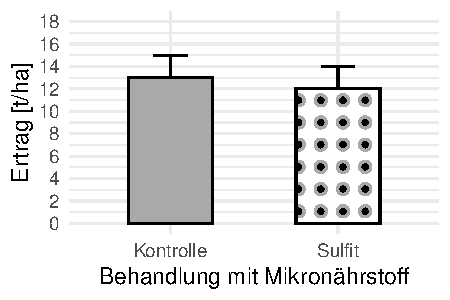
\includegraphics[width=\maxwidth]{img/mc-testing-ttest-02-1} 

}







\begin{enumerate}
\item [\textbf{A} \msquare] Die Barplots deuten auf keinen signifikanten Unterschied. Der Effekt liegt vermutlich bei 3 unter einer groben Abschätzung. Wir müssen aber eine ANOVA rechnen um den Effekt wirklich bestimmen zu können.
\item [\textbf{B} \msquare] Es liegt ein signifikanter Unterschied vor. Der Effekt liegt bei 0.3.
\item [\textbf{C} \msquare] Der Test deutet auf keinen signifikanten Unterschied hin. Der Effekt liegt vermutlich bei 3.
\item [\textbf{D} \msquare] Die Barplots deuten auf einen signifikanten Unterschied. Der Effekt liegt vermutlich bei 3. Wir müssen aber einen Posthoc-Test rechnen um den Effekt wirklich bestimmen zu können.
\item [\textbf{E} \msquare] Der Test deutet auf ein signifikanten Unterschied hin. Der Effekt liegt vermutlich bei 3.
\end{enumerate}

\section{Aufgabe \hfill (2 Punkte)}




In Ihrer Abschlussarbeit betrachten Sie die Effekte von einer Behandlung vor und nach der Gabe eines Vitamins. Sie müssen einen gepaarten t-Test rechnen. Welche Aussage ist richtig?



\begin{enumerate}
\item [\textbf{A} \msquare] Beim gepaarten t-Test kombinieren wir die Vorteile des Student t-Test für Varianzhomogenität mit den Vorteilen des Welch t-Test für Varianzheterogenität. Wir bilden dafür die Differenz der Einzelbeobachtungen.
\item [\textbf{B} \msquare] Wenn die Beobachtungen nicht unabhängig voneinander sind, rechnen wir einen gepaarten t-Test. Messen wir wiederholt an dem gleichen Tier oder Pflanze dann bilden wir die Differenz zwischen den zwei Messpunkten.
\item [\textbf{C} \msquare] Der gepaarte t-Test nutzt die Varianz der Beobachtungen jeweils paarweise und bildet dafür eine verbundene Stichprobe. Dieser Datensatz $d$ dient dann zur Differenzbildung.
\item [\textbf{D} \msquare] Der gepaarte t-Test wird genutzt, wenn die Differenzen der Beobachtungen verbunden sind und wir dadurch die Unabhäängigkeit nicht mehr vorliegen haben.
\item [\textbf{E} \msquare] Abhängige Beobachtungen müssen gesondert in einem gepaarten t-Test modelliert werden. Wenn wiederholt an dem gleichen Tier oder Pflanze gemessen wird, dann bilden wir den Quotienten zwischen den beiden Zeitpunkten. Auf den Quotienten rechnen wir den gepaarten t-Test.
\end{enumerate}

\section{Aufgabe \hfill (2 Punkte)}



Nach einem Experiment mit drei Weizensorten ergibt eine ANOVA ($p = 0.049$) einen signifikanten Unterschied für den Ertrag. Sie führen anschließend die paarweisen t-Tests für alle Vergleiche der verschiedenen Weizensorten durch. Nach der Adjustierung für multiples Testen ist kein p-Wert unter der $\alpha$-Schwelle. Sie schauen sich auch die rohen, unadjustierten p-Werte an und finden hier als niedrigsten p-Wert $p_{3-2} = 0.053$. Welche Aussage ist richtig?




\begin{enumerate}
\item [\textbf{A} \msquare] Der Fehler liegt in den t-Tests. Wenn eine ANOVA signifikant ist, dann muss zwangsweise auch ein t-Test signifikant sein.
\item [\textbf{B} \msquare] Es gibt einen Fehler in der Varianzstruktur. Daher kann die ANOVA nicht richtig sein und paarweise t-Tests liefern das richtige Ergebnis.
\item [\textbf{C} \msquare] Das Beispiel kann so nicht auftreten, da die ANOVA und die t-Tests algorithmisch miteinander verschränkt sind.
\item [\textbf{D} \msquare] Die adjustierten p-Werte deuten in die richtige Richtung. Zusammen mit den nicht signifikanten rohen p-Werten ist von einem Fehler in der ANOVA auszugehen.
\item [\textbf{E} \msquare] Hier kommt der Effekt der stiegenden Fallzahl auf die Anzahl an signifikante Ergebnisse zu tragen. Da die ANOVA auf mehr Fallzahl testet als die einzelnen paarweisen t-Tests, kann die ANOVA leichter einen signifikanten Unterscheid nachweisen. Die p-Werte sind immer etwas kleiner als bei den t-Tests.
\end{enumerate}
    
% -----------------------------------------------------------------------
\clearpage
% -----------------------------------------------------------------------
\part{Deskriptive Statistik \& Explorative Datenanalyse}
% -----------------------------------------------------------------------

\section{Aufgabe \hfill (8 Punkte)}

\textit{Geben Sie grundsätzlich Formeln und Rechenweg zur Lösung der Teilaufgaben mit an!} \\[1Ex]
 

 
%% --------------------------------------------------------------------
\begin{minipage}[t]{0.5\textwidth}

\includegraphics[width = 1.3cm]{/Users/kruppajo/work/GitHub/exam/avatare/Nilufar.png}
\end{minipage}
\begin{minipage}[t]{0.5\textwidth}
\hfill
\href{https://youtu.be/t0WYa_LVc5o}{
\includegraphics[width = 2cm]{img/youtube}}
\end{minipage}
\vspace{-3ex}
%% --------------------------------------------------------------------



\paragraph{Zerforschen des Barplots}

Eine echte Herausforderung für sie war schon immer die Erwartung gewesen. Ein leidiges Lied. Deshalb gilt anschauen, was andere vor einem gemacht haben. Für Nilufar ist es eine Möglichkeit schneller ans Ziel zu gelangen. Nilufar soll in ihrem Projektbericht Erbsen untersuchen. Die Behandlung in ihrem Projektbericht werden verschiedene Düngestufen ($ctrl$, $low$ und $high$) sein. Erheben wird Nilufar als Outcome ($Y$) \textit{Ertrag} benannt als \textit{yield} in ihrer Exceldatei. Von ihrer Betreuer erhält sie nun folgende Abbildung von Barplots, die sie erstmal zur Übung nachbauen soll, bevor sie mit dem eigentlichen Versuch beginnt.



{\centering 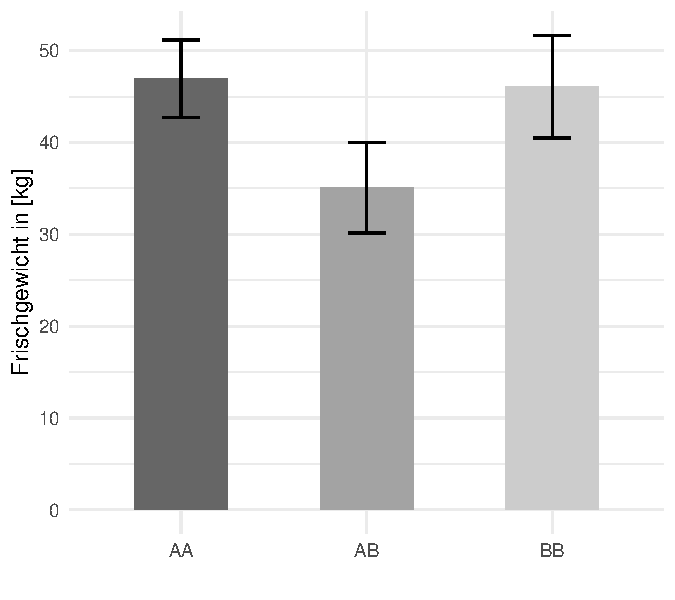
\includegraphics[width=\maxwidth]{img/barplot-02-1} 

}




Leider kennt sich Nilufar mit der Erstellung von Barplots in \Rlogo nicht aus. Deshalb braucht sie bei der Visualisierung Ihre Hilfe!

\begin{enumerate}
\item Formulieren Sie die wissenschaftliche Fragestellung! \textbf{(1 Punkt)}
\item Erstellen Sie eine Tabelle mit den statistischen Maßzahlen der drei Barplots! \textit{Beachten Sie die korrekte Darstellungsform der statistischen Maßzahlen!} \textbf{(3 Punkte)}
\item Erstellen Sie einen beispielhaften Datensatz im \Rlogo üblichen Format, aus dem die drei Barplots \textit{möglicherweise} erstellt wurden! \textbf{(2 Punkte)}
\item Kann Nilufar einen Unterschied zwischen den Behandlungen erwarten? Begründen Sie Ihre Antwort! \textbf{(2 Punkte)}
\end{enumerate} 
\clearpage
% -----------------------------------------------------------------------

\section{Aufgabe \hfill (8 Punkte)}

\textit{Geben Sie grundsätzlich Formeln und Rechenweg zur Lösung der Teilaufgaben mit an!} \\[1Ex]
 

 
%% --------------------------------------------------------------------
\begin{minipage}[t]{0.5\textwidth}

\includegraphics[width = 1.3cm]{/Users/kruppajo/work/GitHub/exam/avatare/Jessica.png}
\end{minipage}
\begin{minipage}[t]{0.5\textwidth}
\hfill
\href{https://youtu.be/vXnLttRL_VI}{
\includegraphics[width = 2cm]{img/youtube}}
\end{minipage}
\vspace{-3ex}
%% --------------------------------------------------------------------



\paragraph{Visualisierung des Barplots}


Jessica steht vor einem ersten Problem, denn wenn es nach ihrem Betreuer geht, soll sie in einem einem Feldexperiment Lauch auswertet. Soweit eigentlich alles passend. Besser wäre was anderes gewesen. Jessica liebt Warhammer. Darin kann sie sich wirklich verlieren und immer wieder neu begeistern. Die Behandlung waren verschiedene Substrattypen ($torf$, $40p60n$ und $70p30n$). In ihrer Exceldatei hat sie den Endpunkt ($Y$) \textit{Trockengewicht} als \textit{drymatter} aufgenommen. Nun soll Jessica die Daten eimal als Barplots in einer Präsentation visualisieren, damit ihrem Betreuer wieder klar wird, was sie eigentlich nochmal gemacht hat und was für ein Ergbnis in einem statistischen Test zu erwarten wäre. Wäre da nicht noch etwas. Eine echte Herausforderung für sie war schon immer der Mangel gewesen. Ein leidiges Lied. Aber egal. Einfach mal raus um Rad zu fahren. Ohne Ziel und Uhr. Das ist was für Jessica.

\begin{table}[!h]
\centering
\begin{tabular}{cc}
\toprule
treatment & drymatter\\
\midrule
70p30n & 41.5\\
torf & 24.6\\
70p30n & 42.6\\
torf & 22.4\\
torf & 32.5\\
\addlinespace
40p60n & 39.5\\
40p60n & 41.8\\
torf & 24.3\\
70p30n & 42.0\\
40p60n & 35.4\\
\bottomrule
\end{tabular}
\end{table}



Leider kennt sich Jessica mit der Erstellung von Barplots nicht aus. Deshalb braucht sie bei der Visualisierung Ihre Hilfe!

\begin{enumerate}
\item Formulieren Sie die wissenschaftliche Fragestellung! \textbf{(1 Punkt)}
\item Zeichnen Sie in \textit{einer} Abbildung die Barplots für die Behandlung von Lauch! Beschriften Sie die Achsen entsprechend!\textbf{(4 Punkte)}
\item Beschriften Sie \textit{einen} Barplot mit den gängigen statistischen Maßzahlen! \textbf{(2 Punkte)}
\item Wenn Jessica \textit{keinen Effekt} zwischen den Behandlungen von Lauch erwarten würde, wie sehen dann die Barplots aus? \textit{Antworten Sie mit einer Skizze der Barplots!}
  \textbf{(1 Punkt)}
\end{enumerate} 
\clearpage
% -----------------------------------------------------------------------

\section{Aufgabe \hfill (9 Punkte)}

\textit{Geben Sie grundsätzlich Formeln und Rechenweg zur Lösung der Teilaufgaben mit an!} \\[1Ex]
 

 
%% --------------------------------------------------------------------
\begin{minipage}[t]{0.5\textwidth}

\includegraphics[width = 1.3cm]{/Users/kruppajo/work/GitHub/exam/avatare/Paula.png}
\end{minipage}
\begin{minipage}[t]{0.5\textwidth}
\hfill
\href{https://youtu.be/Xf0yE-o7bEU}{
\includegraphics[width = 2cm]{img/youtube}}
\end{minipage}
\vspace{-3ex}
%% --------------------------------------------------------------------



\paragraph{Zerforschen des Boxplots}

Paula steht vor einem ersten Problem, denn wenn es nach ihrer Betreuerin geht, soll sie in einem einem Freilandversuch Maiss auswertet. Soweit eigentlich alles passend. Besser wäre was anderes gewesen. Am Ende dann doch besser Harry Potter. Wunderbar. Eine echte Ablenkung für Paula. Das heißt erstmal überlegen für Paula. 'Hm...', Smarties und White Lies. Das ist und bleibt die beste Kombination zum Nachdenken für Paula. Die Behandlung werden verschiedene Bewässerungstypen ($low$, $mid$ und $high$) sein. In ihrer Exceldatei wird sie den Endpunkt ($Y$) \textit{Trockengewicht} als \textit{drymatter} aufnehmen. Vorab soll Paula aber eimal die folgenden Boxplots ihrer Betreuerin nachbauen, damit sie den \Rlogo Code schonmal für später vorliegen hat. Damit geht das Problem schon los. Eine echte Herausforderung für sie war schon immer der Perfektionismus gewesen. Ein leidiges Lied.



{\centering 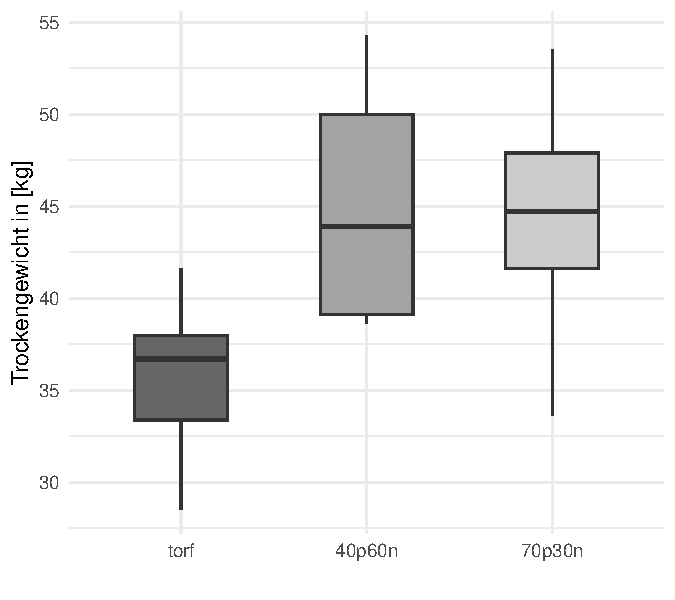
\includegraphics[width=\maxwidth]{img/boxplot-02-zer-1} 

}




Leider kennt sich Paula mit der Erstellung von Boxplots in \Rlogo nicht aus. Deshalb braucht sie bei der Visualisierung Ihre Hilfe!

\begin{enumerate}
\item Erstellen Sie eine Tabelle mit den statistischen Maßzahlen aus der obigen Abbildung der drei Boxplots! \textit{Beachten Sie die korrekte Darstellungsform der statistischen Maßzahlen!} \textbf{(3 Punkte)}
\item Beschriften Sie \textit{einen} der Boxplots mit den gängigen statistischen Maßzahlen! \textbf{(2 Punkte)}
\item Erstellen Sie einen beispielhaften Datensatz, aus dem die drei Boxplots \textit{möglicherweise} erstellt wurden, im \Rlogo üblichen Format! \textbf{(2 Punkte)}
\item Kann Paula einen Unterschied zwischen den Behandlungen erwarten? Begründen Sie Ihre Antwort! \textbf{(2 Punkte)}
\end{enumerate} 
\clearpage
% -----------------------------------------------------------------------

\section{Aufgabe \hfill (9 Punkte)}

\textit{Geben Sie grundsätzlich Formeln und Rechenweg zur Lösung der Teilaufgaben mit an!} \\[1Ex]
 

 
%% --------------------------------------------------------------------
\begin{minipage}[t]{0.5\textwidth}

\includegraphics[width = 1.3cm]{/Users/kruppajo/work/GitHub/exam/avatare/Alex.png}
\end{minipage}
\begin{minipage}[t]{0.5\textwidth}
\hfill
\href{https://youtu.be/0xc0jIPeiyw}{
\includegraphics[width = 2cm]{img/youtube}}
\end{minipage}
\vspace{-3ex}
%% --------------------------------------------------------------------



\paragraph{Visualisierung des Boxplots}

Boxplots sind bedeutend in der Darstellung von wissenschaftlichen Ergebnissen. Leider hat sich Alex nicht gemerkt, welche statistischen Maßzahlen für einen Boxplot erhoben werden müssen. Besser wäre was anderes gewesen. Starcraft. Ein wunderbares Hobby um sich drin zu verlieren und Abstand zu bekommen. Alex denkt gerne über Starcraft nach. Das ist in soweit doof, da nach seinem Betreuer nun Boxplots aus seinen Daten gebaut werden sollen, bevor es mit dem statistischen Testen weitergeht. Anhand von Boxplots lässt sich eine Aussage über die Normalverteilung von $Y$ treffen. Die Behandlung für Maiss waren verschiedene Lüftungssystemen und Folientunneln ($ctrl$ und $tornado$). Erfasst wurde von Alex als Endpunkt ($Y$) \textit{Trockengewicht}. Alex hat dann \textit{drymatter} in seiner Exceldatei eintragen. Aber nur in passender Atmospäre! Schon dutzende Male gesehen: Alien. Aber immer noch großartig zusammen mit Gummibärchen.

\begin{table}[!h]
\centering
\begin{tabular}{cc}
\toprule
treatment & drymatter\\
\midrule
tornado & 37.9\\
tornado & 45.9\\
tornado & 34.5\\
ctrl & 30.8\\
tornado & 44.8\\
\addlinespace
ctrl & 27.9\\
ctrl & 24.2\\
tornado & 38.5\\
ctrl & 24.5\\
tornado & 29.2\\
\addlinespace
ctrl & 21.8\\
tornado & 42.9\\
ctrl & 33.2\\
tornado & 28.8\\
ctrl & 22.0\\
\addlinespace
tornado & 25.4\\
\bottomrule
\end{tabular}
\end{table}



Leider kennt sich Alex mit der Erstellung von Boxplots nicht aus. Deshalb braucht er bei der Visualisierung Ihre Hilfe!

\begin{enumerate}
\item Zeichnen Sie in \textit{einer} Abbildung die beiden Boxplots für die zwei Behandlungen von Maiss! Beschriften Sie die Achsen entsprechend! \textbf{(5 Punkte)} 
\item Wie ist Ihr Vorgehen, wenn Sie eine \textit{gerade} Anzahl an
  Beobachtungen pro Gruppe haben? \textbf{(1 Punkt)}
\item Beschriften Sie \textit{einen} der beiden Boxplots mit den gängigen
  statistischen Maßzahlen! \textbf{(2 Punkte)}
\item Wenn Sie \textit{keinen Effekt} zwischen den Behandlungen von
  Maiss erwarten würden, wie sehen dann die beiden Boxplots aus?
  \textit{Antworten Sie mit einer Skizze der Boxplots!}
  \textbf{(1 Punkt)}
\end{enumerate} 
\clearpage
% -----------------------------------------------------------------------

\section{Aufgabe \hfill (8 Punkte)}

\textit{Geben Sie grundsätzlich Formeln und Rechenweg zur Lösung der Teilaufgaben mit an!} \\[1Ex]
 

 
%% --------------------------------------------------------------------
\begin{minipage}[t]{0.5\textwidth}

\includegraphics[width = 1.3cm]{/Users/kruppajo/work/GitHub/exam/avatare/Jessica.png}
\end{minipage}
\begin{minipage}[t]{0.5\textwidth}
\hfill
\href{https://youtu.be/aXvxGC4YLqk}{
\includegraphics[width = 2cm]{img/youtube}}
\end{minipage}
\vspace{-3ex}
%% --------------------------------------------------------------------



\paragraph{Visualisierung des Histogramm für kategoriale Daten}

Jessica schmeißt noch eine Handvoll Schokobons in ihren Rachen. Im Hintergrund klirrt leise der Spiegel zum Sound von David Bowie. Jessica betrachtet die folgenden Daten nach einem Kreuzungsexperiment mit Zandern. In dem Experiment wurden die dunklen Pigmentstörungen gezählt. Nach der Meinung ihrer Betreuerin muss als erstes geschaut werden, wie diese verteilt sind. Also welcher statistischen Verteilung die dunklen Pigmentstörungen folgen. Dazu soll Jessica ein Histogramm verwenden. Dann hätte man auch einen guten Überblick über das Outcome ($Y$). Es wäre einfacher, wenn da nicht noch was wäre. Jessica und der Mangel, eine unendliche Geschichte mit kniffeligen Wendungen. Jessica nickt im Takt von David Bowie und bemerkt dabei gar nicht was die Hündin schon wieder anstellt.

\begin{center}
Die dunklen Pigmentstörungen: 1, 5, 2, 5, 7, 4, 5, 3, 4, 7, 7, 5, 5, 4, 0, 3, 5, 0, 4, 5, 5, 2, 4, 4, 4, 4, 6, 3, 3, 5, 3, 1, 4
\end{center}

Leider kennt sich Jessica mit der Erstellung von Histogrammen überhaupt nicht aus. Deshalb braucht sie bei der Erstellung Ihre Hilfe!

\begin{enumerate}
\item Zeichen Sie ein Histogramm um die Verteilung der Daten zu visualisieren! (\textbf{3 Punkte})
\item Beschriften Sie die Achsen der Abbildung! (\textbf{2 Punkte})
\item Ergänzen Sie die absoluten und relativen Häufigkeiten in der
  Abbildung! \textbf{(1 Punkt)}
\item Berechnen Sie aus den Daten die \textit{Wahrscheinlichkeit}
  mehr als die Anzahl 4 zu beobachten! \textbf{(1
    Punkt)}
\item Berechnen Sie aus den Daten die \textit{Chance} mehr
  als die Anzahl 4 zu beobachten! \textbf{(1 Punkt)}
\end{enumerate}

 
\clearpage
% -----------------------------------------------------------------------

\section{Aufgabe \hfill (8 Punkte)}

\textit{Geben Sie grundsätzlich Formeln und Rechenweg zur Lösung der Teilaufgaben mit an!} \\[1Ex]
 

 
%% --------------------------------------------------------------------
\begin{minipage}[t]{0.5\textwidth}

\includegraphics[width = 1.3cm]{/Users/kruppajo/work/GitHub/exam/avatare/Jessica.png}
\end{minipage}
\begin{minipage}[t]{0.5\textwidth}
\hfill
\href{https://youtu.be/ORHSPTCdfeY}{
\includegraphics[width = 2cm]{img/youtube}}
\end{minipage}
\vspace{-3ex}
%% --------------------------------------------------------------------



\paragraph{Visualisierung des Histogramm für kontinuierliche Daten}

In ihrer Hausarbeit möchte Jessica gerne die Daten aus einem Kreuzungsexperiment mit Zandern in einem Histogramm darstellen. Das Histogramm erlaubt ihr dabei Rückschlüsse auf die Verteilung über den Messwert ($Y$) zu treffen Jessica schmeißt noch eine Handvoll Schokobons in ihren Rachen. Im Hintergrund klirrt leise der Spiegel zum Sound von David Bowie. In seinem Experiment hat Jessica die mittlere Anzahl an weißen Blutkörperchen gezählt. Es wäre einfacher, wenn da nicht noch was wäre. Eine echte Herausforderung für sie war schon immer der Mangel gewesen. Ein leidiges Lied. Jessica streichelt liebevoll die Hündin. Der Kopf ist in ihrem Schloß vergraben um den Klang von David Bowie zu dämpfen.

\begin{center}
Die mittlere Anzahl an weißen Blutkörperchen: 9.9, 11.5, 4.4, 7.9, 8.5, 7.6, 13, 12.3, 9.9, 8, 11.2, 11.5, 6.6, 10.9, 12.5, 9.1, 10.4, 10.3, 6, 11.7, 8.1, 8.1, 11.1, 12.9, 9
\end{center}

Leider kennt sich Jessica mit der Erstellung von Histogrammen überhaupt nicht aus. Deshalb braucht sie bei der Erstellung Ihre Hilfe!

\begin{enumerate}
\item Zeichen Sie ein Histogramm um die Verteilung der Daten zu visualisieren! (\textbf{3 Punkte})
 \item Erläutern Sie Ihr Vorgehen um ein Histogramm für kontinuierliche Daten zu zeichnen!  (\textbf{2 Punkte})
\item Beschriften Sie die Achsen der Abbildung! (\textbf{2 Punkte})
\item Ergänzen Sie die relativen Häufigkeiten in der Abbildung! \textbf{(1 Punkt)}  
\end{enumerate}

 
\clearpage
% -----------------------------------------------------------------------

\section{Aufgabe \hfill (10 Punkte)}

\textit{Geben Sie grundsätzlich Formeln und Rechenweg zur Lösung der Teilaufgaben mit an!} \\[1Ex]
 

 
%% --------------------------------------------------------------------
\begin{minipage}[t]{0.5\textwidth}

\includegraphics[width = 1.3cm]{/Users/kruppajo/work/GitHub/exam/avatare/Tina.png}
\end{minipage}
\begin{minipage}[t]{0.5\textwidth}
\hfill
\href{https://youtu.be/VAqiUdV4WQ0}{
\includegraphics[width = 2cm]{img/youtube}}
\end{minipage}
\vspace{-3ex}
%% --------------------------------------------------------------------




\paragraph{Visualisierung des Scatterplots}

Wenn es nach Tina ginge, wäre sie schon längst fertig mit ihrer Abschlussarbeit. Geht es aber nicht. Aus den Boxen wummert Tocotronic und ihr Mund ist verklebt von Katjes. 'Herrlich', denkt Tina. In ihrer Abschlussarbeit hatte sie ein Feldexperiment im Teuteburgerwald durchgeführt. Nach der Meinung ihrem Betreuer sieht das jedoch etwas anders aus. Jetzt soll sie doch noch eine explorative Datenanalyse für den Zusammenhang zwischen durchschnittlicher Regenwurmdichte [Anzahl/l] und Proteingehalt [g/kg] in Kartoffeln durchführen. Wie nervig! Wenn die Wut nicht wäre, ja dann wäre wohl vieles möglich für Tina! Aber so.. Da zwei kontinuierliche Variablen vorliegen, geht die explorative Datenanalyse leider nicht mit Boxplots oder Barplots. Dann was anderes. Das Verrückte ist, dass die Spinne Indiana Jones wirklich liebt. Das ist Tina sehr recht, denn sie braucht Entspannung.

\begin{table}[!h]
\centering
\begin{tabular}{cc}
\toprule
Proteingehalt [g/kg] & Durchschnittlicher Regenwurmdichte [Anzahl/l]\\
\midrule
22.1 & 17.7\\
19.9 & 14.4\\
24.4 & 13.6\\
24.2 & 17.6\\
21.4 & 17.7\\
\addlinespace
23.7 & 18.2\\
14.1 & 10.4\\
20.7 & 9.2\\
20.1 & 15.1\\
15.4 & 14.6\\
\bottomrule
\end{tabular}
\end{table}



Leider kennt sich Tina mit der Erstellung einer explorativen Datenanalyse für kontinuierliche Daten überhaupt nicht aus. Deshalb braucht sie bei der Erstellung Ihre Hilfe!

\begin{enumerate}
\item Erstellen Sie eine Visualisierung für die Datentabelle. Beschriften Sie
  die Achsen entsprechend! \textbf{(4 Punkte)}
\item Schätzen Sie eine Gerade durch die Punkte! \textbf{(1 Punkt)}
\item Beschriften Sie die Gerade mit den gängigen statistischen Maßzahlen! Geben Sie die numerischen Zahlenwerte mit an! \textbf{(3 Punkte)}
\item Wenn \textit{ein} Effekt von $x$ auf $y$ vorhanden wäre, wie würde die Gerade verlaufen und welche Werte würden die statistischen Maßzahlen annehmen? \textbf{(2 Punkt)}
\end{enumerate} 
\clearpage
% -----------------------------------------------------------------------

\section{Aufgabe \hfill (10 Punkte)}

\textit{Geben Sie grundsätzlich Formeln und Rechenweg zur Lösung der Teilaufgaben mit an!} \\[1Ex]
 

 
%% --------------------------------------------------------------------
\begin{minipage}[t]{0.5\textwidth}

\includegraphics[width = 1.3cm]{/Users/kruppajo/work/GitHub/exam/avatare/Paula.png}
\end{minipage}
\begin{minipage}[t]{0.5\textwidth}
\hfill
\href{https://youtu.be/t_1KL77mfmg}{
\includegraphics[width = 2cm]{img/youtube}}
\end{minipage}
\vspace{-3ex}
%% --------------------------------------------------------------------



\paragraph{Visualisierung des Mosaicplots}

Wenn Jagd auf roter Oktober läuft, dann ist die Ratte nicht mehr da. Aber jetzt braucht sie mal Entspannung! Aber Ablenkung hilft nur begrenzt. 'Uff!', denkt sich Paula. Jetzt hat sie doch tatsächlich zwei kategoriale Variablen in ihrer Abschlussarbeit gemessen. Zum einen die Behandlung Klimakontrolle [ja/nein] und zum anderen die Messung Gewichtszuwachs erreicht [ja/nein] im Kontext von Puten. Hierfür hat sie ein Kreuzungsexperiment im Emsland durchgeführt. Jetzt möchte Paula die Daten einmal in einer explorativen Datenanalyse darstellen. Danach kann sie dann über den passenden statistischen Test nachdenken. Dabei unterstützt ihre Betreuerin diesen Ansatz bevor es in der Datenanalyse weiter geht. So schön wie so gut. Wenn der Perfektionismus nicht wäre, ja dann wäre wohl vieles möglich für Paula! Aber so..



\vspace{1Ex}

\begin{center}
\begin{minipage}[t]{0.45\textwidth}
%\small
\begin{center}

\begin{tabular}{p{2.5cm}p{2.5cm}p{2.5cm}p{2.5cm}}
\toprule
Gewichtszuwachs erreicht & Klimakontrolle\\
\midrule
ja & nein\\
nein & nein\\
ja & ja\\
ja & ja\\
nein & nein\\
\addlinespace
nein & ja\\
ja & nein\\
nein & ja\\
ja & nein\\
nein & ja\\
\addlinespace
nein & ja\\
nein & ja\\
nein & nein\\
nein & ja\\
ja & nein\\
\addlinespace
ja & nein\\
nein & ja\\
ja & nein\\
\bottomrule
\end{tabular}


\end{center}
\end{minipage}
\begin{minipage}[t]{0.45\textwidth}
%\small
\begin{center}

\begin{tabular}{p{2.5cm}p{2.5cm}p{2.5cm}p{2.5cm}}
\toprule
Gewichtszuwachs erreicht & Klimakontrolle\\
\midrule
ja & nein\\
nein & nein\\
ja & nein\\
ja & ja\\
ja & nein\\
\addlinespace
nein & nein\\
ja & ja\\
ja & nein\\
ja & nein\\
nein & nein\\
\addlinespace
ja & nein\\
nein & ja\\
nein & nein\\
ja & ja\\
nein & ja\\
\addlinespace
ja & nein\\
nein & nein\\
nein & ja\\
\bottomrule
\end{tabular}


\end{center}
\end{minipage}
\end{center}

\vspace{2Ex}

Leider kennt sich Paula mit der Erstellung einer explorativen Datenanalyse für kategoriale Daten überhaupt nicht aus. Deshalb braucht sie bei der Erstellung Ihre Hilfe!

\begin{enumerate}
\item Stellen Sie den Zusammenhang zwischen den beiden kategorialen Variablen in einer zusammenfassenden Tabelle dar! \textbf{(3 Punkte)}
\item Visualisieren Sie den Zusammenhang zwischen den beiden kategorialen Variablen! \textbf{(3 Punkte)}
\item Berechnen Sie die Verhältnisse in der Visualisierung! Welche Annahme haben Sie getroffen? \textbf{(2 Punkte)}
\item Wenn \textit{ein} Effekt von der Behandlung vorliegen würde, wie würde die Tabelle und die Visualisierung aussehen? \textbf{(2 Punkt)}
\end{enumerate} 
\clearpage
% -----------------------------------------------------------------------

\section{Aufgabe \hfill (10 Punkte)}

\textit{Geben Sie grundsätzlich Formeln und Rechenweg zur Lösung der Teilaufgaben mit an!} \\[1Ex]
 

 
%% --------------------------------------------------------------------
\begin{minipage}[t]{0.5\textwidth}

\includegraphics[width = 1.3cm]{/Users/kruppajo/work/GitHub/exam/avatare/Alex.png}\hspace{-4mm}
\includegraphics[width = 1.3cm]{/Users/kruppajo/work/GitHub/exam/avatare/Steffen.png}
\end{minipage}
\begin{minipage}[t]{0.5\textwidth}
\hfill
\href{https://youtu.be/Op-gjzASH9I}{
\includegraphics[width = 2cm]{img/youtube}}
\end{minipage}
%% --------------------------------------------------------------------



\paragraph{Visualisierung von Verteilungen}

'Was soll das denn jetzt schon wieder sein? Drei Boxplot, die auf der Seite liegen?', entfährt es Alex und schaut dabei Steffen an. 'Keine Ahnung. Es ist bestimmt wieder so ein Lernziel mit der Verteilung und so.', meint Steffen sichtlich genervt und mampft noch ein paar Oreos. 'Du weißt doch wie es heißt, \textit{Frei ist, wer missfallen kann.}\footnote{Oschmann, A. (2024) Mädchen stärken: Stärken fördern, Selbstwert erhöhen und liebevoll durch Krisen begleiten. Goldegg Verlag}', merkt Alex nickend an. Die beiden schauen angestrengt auf die drei Boxplots. Das Ziel ist es zu verstehen, wie eine Verteilung anhand eines Boxplots bewertet werden kann. Steffen und die Romantik machen die Sache nicht einfacher.



{\centering 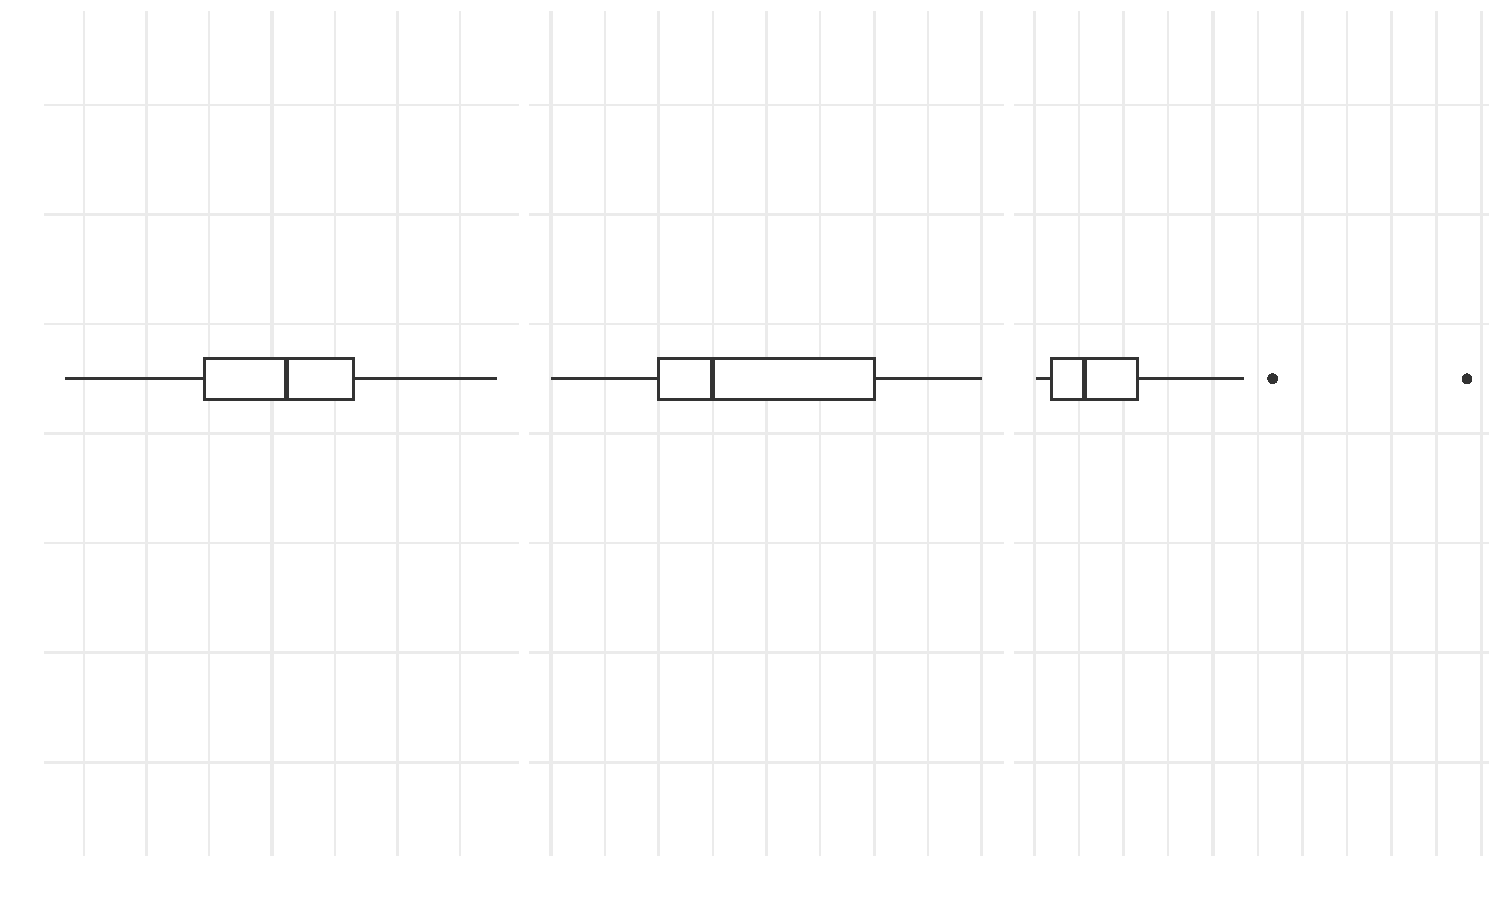
\includegraphics[width=\maxwidth]{img/desc-stat-11-1} 

}




Jetzt brauchen Alex und Steffen Ihre Hilfe bei der Abschätzung einer Verteilung anhand von Boxplots um ihre Arbeit dann in diesem Semester noch abschließen zu können.

\begin{enumerate}
\item Zeichnen Sie über die Boxplots die entsprechende zugehörige Verteilung! \textbf{(3 Punkte)} 
\item Zeichnen Sie unter die Boxplots die entsprechende zugehörige Beobachtungen als Stiche! \textbf{(3 Punkte)}
\item Wie viel Prozent der Beobachtungen fallen in das IQR? Ergänzen Sie die Abbildung entsprechend um den Bereich! \textbf{(2 Punkte)}
\item Wie viel Prozent der Beobachtungen fallen in $\bar{y} \pm 1s$ und $\bar{y} \pm 2s$  unter der Annahme einer Normalverteilung? \textbf{(2 Punkte)}
\end{enumerate} 
\clearpage
% -----------------------------------------------------------------------

\section{Aufgabe \hfill (10 Punkte)}

\textit{Geben Sie grundsätzlich Formeln und Rechenweg zur Lösung der Teilaufgaben mit an!} \\[1Ex]
 

 
%% --------------------------------------------------------------------
\begin{minipage}[t]{0.5\textwidth}

\includegraphics[width = 1.3cm]{/Users/kruppajo/work/GitHub/exam/avatare/Alex.png}\hspace{-4mm}
\includegraphics[width = 1.3cm]{/Users/kruppajo/work/GitHub/exam/avatare/Jonas.png}
\end{minipage}
\begin{minipage}[t]{0.5\textwidth}
\hfill
\href{https://youtu.be/ZrJhn2wPbq4}{
\includegraphics[width = 2cm]{img/youtube}}
\end{minipage}
%% --------------------------------------------------------------------



\paragraph{Visualisierung der Normalverteilung}

Alex und die Gefälligkeit machen die Sache mit dem Studium nicht einfacher. Immerhin ist noch Jonas zur Hilfe mit dabei. Jonas hat Snickers mitgebracht und Iron Maiden aufgedreht. Das ist immerhin eine Ablenkung. Nicht so gut wie Starcraft, aber immerhin etwas. Jetzt sollen die beiden diese komische Aufgabe lösen. Es geht um verschiedene Normalverteilungen. Anscheinend hängen Normalverteilungen vom Mittelwert $\bar{y}$ und der Standardabweichung $s$ ab. 'Wozu brauchen wir nochmal Normalverteilungen?', entfährt es Alex. Durch das Mampfen von Jonas versteht er kein Wort der Antwort. Jonas lächelt.\\



Jetzt brauchen Alex und Jonas Ihre Hilfe bei der Abschätzung einer Verteilung um ihre Arbeit dann in diesem Semester noch abschließen zu können.

\begin{enumerate}
\item Skizzieren Sie zwei Normalverteilungen mit $\bar{y}_1 \neq \bar{y}_2$ und $s_1 \neq s_2$! \textbf{(3 Punkte)}
\item Beschriften Sie die Normalverteilungen mit den statistischen Maßzahlen! \textbf{(2 Punkte)}
\item Liegt Varianzhomogenität oder Varianzheterogenität vor? Begründen Sie Ihre Antwort! \textbf{(2 Punkte)}
\item In welchen Bereich fallen 68\% bzw. 95\% der Beobachtungen in einer Normalverteilung? Ergänzen Sie die Bereiche in \underline{einer} Normalverteilung! \textbf{(2 Punkte)}
\item Ergänzen Sie unter \underline{einer} der Normalverteilungen den entsprechenden Boxplot! \textbf{(1 Punkt)}
\end{enumerate}

 
\clearpage
% -----------------------------------------------------------------------

\section{Aufgabe \hfill (10 Punkte)}

\textit{Geben Sie grundsätzlich Formeln und Rechenweg zur Lösung der Teilaufgaben mit an!} \\[1Ex]
 

 
%% --------------------------------------------------------------------
\begin{minipage}[t]{0.5\textwidth}

\includegraphics[width = 1.3cm]{/Users/kruppajo/work/GitHub/exam/avatare/Jessica.png}\hspace{-4mm}\includegraphics[width = 1.3cm]{/Users/kruppajo/work/GitHub/exam/avatare/Mark.png}
\end{minipage}
\begin{minipage}[t]{0.5\textwidth}
\hfill
\href{https://youtu.be/MiD42k4l5Ag}{\includegraphics[width = 2cm]{img/youtube}}
\end{minipage}
%% --------------------------------------------------------------------



\paragraph{Visualisierung der Normalverteilung und der Poissonverteilung}

'Was zum Geier?!', entfährt es Jessica und schaut dabei Mark an. Dabei nimmt sogar die Hündin reißaus und versteckt sich unter dem Bett. 'Wir sollen eine Normalverteilung mit einem Mittelwert von $\bar{y}_1 = 3$ und einer Standardabweichung von $s_1 = 0.25$ zeichnen. Sowie eine weitere Normalverteilung mit einem Mittelwert von $\bar{y}_2 = 2$ und einer Standardabweichung von $s_2 = 0.25$. Keine Ahnung wie das geht. Darunter sollen dann noch eine Poissonverteilung mit einem Mittelwert von $\lambda_1 = 25$ sowie einer weiteren Poissonverteilung mit einem Mittelwert von $\lambda_2 = 3$ gezeichnet werden.', meint Mark sichtlich genervt und mampft noch ein paar Marzipankugeln. Mark und die Unsicherheit machen die Suche nach der Lösung nicht einfacher. Im Hintergrund spielt viel zu leise Andrea Berg, die diesmal Mark ausgewählt hat.\\




{\centering \includegraphics[width=\maxwidth]{img/histogram-01-1} 

}




Jetzt brauchen Jessica und Mark Ihre Hilfe bei der Abschätzung einer Verteilung um ihre Arbeit dann in diesem Semester noch abschließen zu können.


\begin{enumerate}
\item Skizzieren Sie die zwei Normalverteilungen und zwei Poissonverteilungen! \textbf{(4 Punkte)}
\item Achten Sie auf die entsprechende Skalierung in den jeweiligen Abbildungen! \textbf{(2 Punkte)}
\item Ergänzen Sie unter \underline{einer} Normalverteilung den entsprechenden Boxplot! \textbf{(1 Punkt)}
\item Ergänzen Sie unter \underline{einer} Poissonverteilung den entsprechenden Boxplot! \textbf{(1 Punkt)}
\item Geben Sie ein Beispiel für ein Outcome $y$, welches einer Normalverteilung folgt! \textbf{(1 Punkt)}
\item Geben Sie ein Beispiel für ein Outcome $y$, welches einer Poissonverteilung folgt! \textbf{(1 Punkt)}
\end{enumerate} 
\clearpage
% -----------------------------------------------------------------------
\part{Statistisches Testen \& statistische Testtheorie}
% -----------------------------------------------------------------------  

\section{Aufgabe \hfill (9 Punkte)}


 
%% --------------------------------------------------------------------
\begin{minipage}[t]{0.5\textwidth}
\includegraphics[width = 1.3cm]{/Users/kruppajo/work/GitHub/exam/avatare/Tina.png}\hspace{-4mm}\includegraphics[width = 1.3cm]{/Users/kruppajo/work/GitHub/exam/avatare/Yuki.png}
\end{minipage}
\begin{minipage}[t]{0.5\textwidth}
\hfill
\href{https://youtu.be/aHVYuFKTqZs}{\includegraphics[width = 2cm]{img/youtube}}
\end{minipage}
%% --------------------------------------------------------------------



\paragraph{Grundgesamtheit und experimentelle Stichprobe}

An einem schwülem Sommernachmittag sitzen Tina und Yuki in einem Eiskaffee und wollen sich auf die Klausur vorbereiten. In fast allen Fragen geht es ja um die Interpretation eines statistischen Tests. Daher wollen die beiden jetzt nochmal nacharbeiten, was die Grundlagen der Stichprobe (eng. \textit{sample}) und der Grundgesamtheit (eng. \textit{population} oder \textit{ground truth}) sind. Tina hat sich Katjes Eisbecher bestellt und Yuki bleibt lieber bei einem Reese's Peanut Butter Cups Eis. 'Irre, was die Lebensmittelindustrie alles auf die Beine kriegt', merk Yuki an und Tina schüttelt anerkennend den Kopf.

\vspace{1ex}

Leider kennen sich Tina und Yuki mit der Grundgesamtheit und der Stuchprobe überhaupt nicht aus. Daher sind Sie gefragt!

\begin{enumerate}
\item Nennen Sie das statistische Verfahren und zwei konkrete Beispiele zur Durchführung um von einer Grundgesamtheit auf eine Stichprobe zu gelangen! \textbf{(3 Punkte)}
\item Erklären Sie den Zusammenhang zwischen Stichprobe und Grundgesamtheit an einem Schaubild! Beschriften Sie das Schaubild entsprechend!
  \textit{Nutzen Sie hierfür als Veranschaulichung die Körpergröße von Männern oder Frauen aus den Gummibärchendaten!}  \textbf{(3 Punkte)}
\item Erweitern Sie das Schaubild um die Entstehung von $Pr(D|H_0)$! \textit{Nutzen Sie hierfür als Veranschaulichung zusätzlich die Gruppierungsvariable "`Modul"' aus den Gummibärchendaten!}  \textbf{(3 Punkte)}
\end{enumerate} 
\clearpage
% -----------------------------------------------------------------------

\section{Aufgabe \hfill (9 Punkte)}


 
%% --------------------------------------------------------------------
\begin{minipage}[t]{0.5\textwidth}
\includegraphics[width = 1.3cm]{/Users/kruppajo/work/GitHub/exam/avatare/Jessica.png}\hspace{-4mm}\includegraphics[width = 1.3cm]{/Users/kruppajo/work/GitHub/exam/avatare/Yuki.png}
\end{minipage}
\begin{minipage}[t]{0.5\textwidth}
\hfill
\href{https://youtu.be/Ric8ne39DtI}{\includegraphics[width = 2cm]{img/youtube}}
\end{minipage}
%% --------------------------------------------------------------------



\paragraph{Das Nullritual - Die statistische Testtheorie}

'Herr der Ringe ist der beste Film, den es gibt.', meint Jessica. Yuki entgegnet, ' Ich empfehle ja immer allen Matrix.'Die beiden sind im Zoo und diskutieren, ob Pinguine Knie haben. Eigentlich wollten beide nochmal die statistische Testheorie durchgehen, sind dann aber auf abenteuerlichen Wege im Zoo gelandet. Jessica starrt wie hypnotisiert auf einen strullenden Elefanten und stopt die Zeit.\footnote{Yang, P. J., et al. (2014). Duration of urination does not change with body size. Proceedings of the National Academy of Sciences, 111(33), 11932-11937.} 'Du bist so peinlich.', entfährt es Yuki und schmeißt sich noch ein paar überteuerte Reese's Peanut Butter Cups rein.

\vspace{1ex}

Leider kennen sich Jessica und Yuki mit statistischen Testtheorie, auch Null-Ritual genannt, überhaupt nicht aus. Geschweige denn mit der Visualisierung als Kreuztabelle.  

\begin{enumerate}
\item Tragen Sie folgende statistische Fachbegriffe zur statistischen Testtheorie korrekt eine selbst erstellte Kreuztabelle ein! \textbf{(3 Punkte)}
  \begin{center}
  \begin{tabular}{cccc}
  Testentscheidung & $\alpha$-Fehler & H$_0$ falsch & H$_0$ abgelehnt \\
  \end{tabular}
  \end{center}
\item Ergänzen Sie Ihre erstellte Kreuztabelle um vier weitere, passende Fachbegriffe zur statistischen Testtheorie! \textbf{(2 Punkte)}
\end{enumerate}

Die Entscheidungsfindung durch einen statistischen Test kann auch durch die Analogie zu einem Feuermelder abgebildet werden. Dabei symbolisiert der Feuermelder den statistischen Test und es soll getestet werden, ob ein Feuer ausgebrochen ist.

\begin{enumerate}
  \setcounter{enumi}{2}    
\item In der Analogie des Feuermelders, wie lautet der $\alpha$-Fehler? \textbf{(1 Punkt)}
\item In der Analogie des Feuermelders, wie lautet der $\beta$-Fehler? \textbf{(1 Punkt)}
\item Wenn der Feuermelder einmal pro Tag messen würde, wie oft würde der Feuermelder mit einem $\alpha$ von 5\% in einem halben Jahr Alarm schlagen? Begründen Sie Ihre Antwort! \textbf{(2 Punkte)}
\end{enumerate}



 
\clearpage
% -----------------------------------------------------------------------

\section{Aufgabe \hfill (9 Punkte)}

\textit{Geben Sie grundsätzlich Formeln und Rechenweg zur Lösung der Teilaufgaben mit an!} \\[1Ex]


 
%% --------------------------------------------------------------------
\begin{minipage}[t]{0.5\textwidth}
\includegraphics[width = 1.3cm]{/Users/kruppajo/work/GitHub/exam/avatare/Paula.png}\hspace{-4mm}\includegraphics[width = 1.3cm]{/Users/kruppajo/work/GitHub/exam/avatare/Steffen.png}
\end{minipage}
\begin{minipage}[t]{0.5\textwidth}
\hfill
\href{https://youtu.be/32JjH1eyuTU}{\includegraphics[width = 2cm]{img/youtube}}
\end{minipage}
%% --------------------------------------------------------------------



\paragraph{Visualisierung der Teststatistik $\boldsymbol{T_D}$ und dem p-Wert}

'Wir sollen die Teststatistik $T_D$ umd dem p-Wert visualisieren, da mit einer Visualisierung vieles verständlicher wird!', ruft Steffen um Taylor Swift zu übertönen. 'Ich weiß nicht, was das jetzt helfen soll. Können wir nicht einfach schauen, ob der p-Wert kleiner als das Signifikanzniveau  $\alpha$ gleich 5\% ist? Und gut ist?', merkt Paula an, was aber im Refrain von Taylor Swift untergeht. Steffen nickt im Beat. 'Wir haben hier eine t-verteilung unter der Annahme der Nullhypothese!', singt er.

\vspace{1ex}

Leider kennen sich Steffen und Paula mit der Visualisierung der Teststatistik $T_D$ und dem p-Wert überhaupt nicht aus und brauchen dahr Ihre Hilfe!

\vspace{1ex}

\textit{Beachten Sie, dass im Folgenden \underline{keine numerisch korrekte Darstellung} verlangt wird! Es gilt Erkennbarkeit vor Genauigkeit!}

\begin{enumerate}
\item Ergänzen Sie eine beschriftete $x$-Achse! \textbf{(1 Punkt)}
\item Ergänzen Sie "`$\bar{y}_1 = \bar{y}_2$"'! \textbf{(1 Punkt)} 
\item Ergänzen Sie "`$A = 0.95$"'! \textbf{(1 Punkt)}
\item Zeichnen Sie $T_{\alpha=5\%}$ in die Abbildung! \textbf{(1 Punkt)} 
\item Zeichnen Sie das Signifikanzniveau $\alpha$ in die Abbildung! Begründen Sie Ihre Antwort! \textbf{(2 Punkte)} 
\item Zeichnen Sie $+T_{D}$ in die Abbildung! \textbf{(1 Punkt)}
\item Zeichnen Sie einen signifikant p-Wert in die Abbildung! Begründen Sie Ihre Antwort! \textbf{(2 Punkte)}   
\end{enumerate}



{\centering \includegraphics[width=\maxwidth]{img/statistisches-testen-3-1} 

}


 
\clearpage
% -----------------------------------------------------------------------

\section{Aufgabe \hfill (10 Punkte)}


 
%% --------------------------------------------------------------------
\begin{minipage}[t]{0.5\textwidth}
\includegraphics[width = 1.3cm]{/Users/kruppajo/work/GitHub/exam/avatare/Alex.png}\hspace{-4mm}\includegraphics[width = 1.3cm]{/Users/kruppajo/work/GitHub/exam/avatare/Mark.png}
\end{minipage}
\begin{minipage}[t]{0.5\textwidth}
\hfill
\href{https://youtu.be/CN_O4fYPbhs}{\includegraphics[width = 2cm]{img/youtube}}
\end{minipage}
%% --------------------------------------------------------------------



\paragraph{Visualisierung des 95\% Konfidenzintervalls}

'So, was haben wir gemacht? Wir haben einen t-test für den Vergleich der Mittelwerte gerechnet.', meint Mark. Alex schaut fragend. 'Hatten wir nicht alles zu einer Kontrolle verglichen? Das war doch so!', ruft Alex laut aus. 'Wir haben doch Messwert \textit{Energieverbrauch der Klimakammer} erhoben.', stellt Mark fest. Jetzt haben beide das Problem, die möglichen 95\% Konfidenzintervalle zu interpretieren.

\vspace{1ex}

Leider kennen sich Mark und Alex mit der Visualisierung des 95\% Konfidenzintervall überhaupt nicht aus. 

\begin{enumerate}
\item Beschriften Sie die untenstehende Abbildung mit der Signifikanzschwelle! Begründen Sie Ihre Antwort! \textbf{(2 Punkte)}
\item Ergänzen Sie eine \textit{in den Kontext passende} Relevanzschwelle! Begründen Sie Ihre Antwort! \textbf{(2 Punkte)} 
\item Skizieren Sie in die untenstehende Abbildung sechs einzelne Konfidenzintervalle (a-f) mit den
  jeweiligen Eigenschaften! \textbf{(6 Punkte)}
  \begin{itemize}
  \item[(a)] Ein nicht signifikantes, nicht relevantes 95\% Konfidenzintervall 	
  \item[(b)] Ein signifikantes, relevantes 90\% Konfidenzintervall. 	
  \item[(c)] Ein 95\% Konfidenzintervall mit h{"o}herer Fallzahl $n$ in der Stichprobe als der Rest der 95\% Konfidenzintervalle 	
  \item[(d)] Ein signifikantes, nicht relevantes 95\% Konfidenzintervall 
  \item[(e)] Ein signifikantes, relevantes 95\% Konfidenzintervall
  \item[(f)] Ein 95\% Konfidenzintervall mit niedriger Fallzahl $n$ in der Stichprobe als der Rest 95\% der Konfidenzintervalle
  \end{itemize}
\end{enumerate}

\begin{center}
  \includegraphics[height = 10cm]{/Users/kruppajo/work/GitHub/exam/question/img/statistisches-testen-04}
\end{center}


 
\clearpage
% -----------------------------------------------------------------------

\section{Aufgabe \hfill (10 Punkte)}

\textit{Geben Sie grundsätzlich Formeln und Rechenweg zur Lösung der Teilaufgaben mit an!} \\[1Ex]


 
%% --------------------------------------------------------------------
\begin{minipage}[t]{0.5\textwidth}
\includegraphics[width = 1.3cm]{/Users/kruppajo/work/GitHub/exam/avatare/Alex.png}\hspace{-4mm}\includegraphics[width = 1.3cm]{/Users/kruppajo/work/GitHub/exam/avatare/Jonas.png}
\end{minipage}
\begin{minipage}[t]{0.5\textwidth}
\hfill
\href{https://youtu.be/FgZmpnEWDag}{\includegraphics[width = 2cm]{img/youtube}}
\end{minipage}
%% --------------------------------------------------------------------



\paragraph{Zusammenhang zwischen dem Effekt, der Streuung sowie der Fallzahl}

An einem kalten Dezembermorgen haben sich Jonas und Alex zum Lernen verabredet. Eine große Kanne Tee und Berge von Snickers warten darauf gegessen zu werden. Jonas liest laut vor:\begin{quote}
                 \textit{
                 Beim statistischen Testen gibt es einen Zusammenhang zwischen dem Effekt, der Streuung sowie der Fallzahl. Gegeben sei die Formel für den Student t-Test auf den die folgenden Überlegungen basieren sollen. Welche Auswirkung hat die Änderungen der jeweiligen statistischen Maßzahl des Effekts $\Delta$, der Streuung $s$ und der Fallzahl $n$ auf die Teststistik $T_{D}$, den p-Wert $Pr(D|H_0)$ sowie dem Konfidenzintervall $KI_{1-\alpha}$?
                 }
                 \end{quote}Alex hebt die Augenbraue. 'Irgendwie sagt mir die Aufgabe jetzt mal so gar nichts. Was soll da gemacht werden?', merkt Alex an und ergänzt: 'Schauen wir doch erstmal zur Entspannung Alien, den Film habe ich extra nochmal mitgebracht.' Jonas ist der Idee nicht abgeneigt und auch das Meerschweinchen kommt unter dem Sofa hervor um mitzuschauen. 

\vspace{1ex}

Leider kennen sich Jonas und Alex mit dem Zusammenhang zwischen dem Effekt, der Streuung sowie der Fallzahl überhaupt nicht aus. 


\begin{enumerate}
\item Visualisieren Sie den Zusammenhang zwischen der Teststatiatik $T_{D}$ und dem p-Wert $Pr(D|H_0)$ für sich verändernde $T_{D}$-Werte!\textit{Geben Sie dafür ein numerisches Beispiel in dem Sie drei $T_{D}$-Werte und deren Einfluss auf den p-Wert vergleichen!} \textbf{(3 Punkte)}  
\item  Füllen Sie die untenstehende Tabelle aus in dem Sie die Änderung der statistischen Maßzahlen auf die Teststatistik, den p-Wert sowie das Konfidenzintervall in \textit{einem} Wort oder Symbol beschreiben! \textbf{(4 Punkte)}
\begin{center}
  \large
  \begin{tabular}[c]{l|c|c|c|l|c|c|c}
    & $T_{D}$ & $Pr(D|H_0)$ & $KI_{1-\alpha}$ & & $T_{D}$ & $Pr(D|H_0)$ & $KI_{1-\alpha}$\strut\\ 
    \hline
    \textbf{$\Delta\; \uparrow$} & \hspace{1.8cm} & \hspace{1.8cm}  & \hspace{1.8cm} & \textbf{
                                                          $\Delta\; \downarrow$} &
                                                                          \hspace{1.8cm} & \hspace{1.8cm}  & \hspace{1.8cm}\strut\\
    \hline
        \textbf{$s\; \uparrow$} & \hspace{1.8cm} & \hspace{1.8cm}  & \hspace{1.8cm} & \textbf{
                                                          $s\; \downarrow$} &
                                                                          \hspace{1.8cm}
                                                & \hspace{1.8cm}  & \hspace{1.8cm}\strut\\
    \hline
        \textbf{$n\; \uparrow$} & \hspace{1.8cm} & \hspace{1.8cm}  & \hspace{1.8cm} & \textbf{
                                                          $n\; \downarrow$} &
                                                                          \hspace{1.8cm}
                                                & \hspace{1.8cm}  & \hspace{1.8cm}\strut\\
    \hline
  \end{tabular}
\end{center}
\item Visualisieren Sie ein 95\%-iges Konfidenzintervall im Vergleich zu einem 90\%-igen Konfidenzintervall! Begründen Sie Ihre Visualisierung anhand der Formel des Konfidenzintervalls des t-Tests mathematisch! \textbf{(3 Punkte)} 
\end{enumerate} 
\clearpage
% -----------------------------------------------------------------------
\part{Der Student t-Test, Welch t-Test \& gepaarter t-Test}
% -----------------------------------------------------------------------

\section{Aufgabe \hfill (9 Punkte)}

\textit{Geben Sie grundsätzlich Formeln und Rechenweg zur Lösung der Teilaufgaben mit an!} \\[1Ex]
 

 
%% --------------------------------------------------------------------
\begin{minipage}[t]{0.5\textwidth}
\includegraphics[width = 1.3cm]{/Users/kruppajo/work/GitHub/exam/avatare/Paula.png}
\end{minipage}
\begin{minipage}[t]{0.5\textwidth}
\hfill
\href{https://youtu.be/eejS2uG4o-M}{\includegraphics[width = 2cm]{img/youtube}}
\end{minipage}
\vspace{-3ex}
%% --------------------------------------------------------------------



\paragraph{Berechnung des Student t-Test \underline{oder} Welch t-Test}

Der t-Test. Paula erschaudert. Eine echte Herausforderung für sie war schon immer der Perfektionismus gewesen. Ein leidiges Lied. Ein mächtiges Werkzeug ist der t-Test in den Händen desjenigen, der einen normalverteilten Endpunkt ($Y$) hat. Aber erstmal überhaupt den t-Test rechnen können. Wie sah das Experiment von Paula überhaupt aus? Aus den Boxen wummert White Lies und ihr Mund ist verklebt von Smarties. 'Herrlich', denkt Paula. Paula hat ein Feldexperiment mit Kartoffeln durchgeführt um eine neue technische Versuchsanlage zu testen. Bei dem Pilotexperiment mit sehr geringer Fallzahl $(n_1 = n_2 = 3)$ wurde die Behandlung Genotypen ($AA$ und $BB$) an den Kartoffeln getestet und dabei wurde geschaut, ob der Versuch überhaupt technisch klappen könnte. Gemessen hat Paula dann als Messwert Trockengewicht [kg/ha]. Warum der Versuch in der Uckermark für ihre Abschlussarbeit stattfinden musste, ist ihr bis heute ein Rätsel. Egal. Gibt es jetzt einen Zusammenhang zwischen der Behandlung und Trockengewicht [kg/ha]?

\begin{table}[!h]
\centering
\begin{tabular}{cc}
\toprule
treatment & weight\\
\midrule
dose & 15.9\\
ctrl & 14.2\\
dose & 18.6\\
dose & 11.4\\
ctrl & 15.4\\
\addlinespace
ctrl & 14.8\\
\bottomrule
\end{tabular}
\end{table}



Leider kennt sich Paula mit der Berechnung eines t-Tests überhaupt nicht aus. Deshalb braucht sie bei der Berechnung Ihre Hilfe!

\begin{enumerate}
  \item Formulieren Sie die wissenschaftliche Fragestellung! \textbf{(1 Punkt)}
  \item Bestimmen Sie die Teststatistik $T_{D}$ eines Student t-Tests! \textbf{(3 Punkte)}
  \item Treffen Sie mit $T_{\alpha = 5\%} = 1.96$ eine Aussage zur Nullhypothese! Begründen Sie Ihre Antwort! \textbf{(2 Punkte)}
  \item Berechnen Sie den Effekt des Student t-Tests! \textbf{(1 Punkt)}
  \item Formulieren Sie eine Antwort an Paula über das Ergebnis Ihrer statistischen Analyse! \textbf{(2 Punkte)}
\end{enumerate} 
\clearpage
% -----------------------------------------------------------------------

\section{Aufgabe \hfill (12 Punkte)}

\textit{Geben Sie grundsätzlich Formeln und Rechenweg zur Lösung der Teilaufgaben mit an!} \\[1Ex]
 

 
%% --------------------------------------------------------------------
\begin{minipage}[t]{0.5\textwidth}
\includegraphics[width = 1.3cm]{/Users/kruppajo/work/GitHub/exam/avatare/Jonas.png}
\end{minipage}
\begin{minipage}[t]{0.5\textwidth}
\hfill
\href{https://youtu.be/Cq_rF_z4xOk}{\includegraphics[width = 2cm]{img/youtube}}
\end{minipage}
\vspace{-3ex}
%% --------------------------------------------------------------------



\paragraph{Berechnung des Student t-Test}

'Der t-Test testet ein normalverteiltes Outcome ($Y$).', liest Jonas laut. Das hilft jetzt auch nur bedingt weiter. Wenn die Erschöpfung nicht wäre, ja dann wäre wohl vieles möglich für Jonas! Aber so.. Laut seiner Betreuerin ist zwar ihm Messwert Fettgehalt [\%/kg] normalverteilt, aber wie rechnet er jetzt einen t-Test? Für seinen Projektbericht musste er ein Stallexperiment mit Milchvieh im Teuteburgerwald durchführen. Als wäre das nicht schon anstrengend genug gewesen. Jetzt soll er auch noch testen, ob die Behandlung Lüftungssystem ($keins$ und $vorhanden$) ein signifikantes Ergebnis liefert. Hm..., was entspannendes wäre gut. Hm, lecker Snickers und dazu dann im Hintergrund Mission Impossible laufen lassen.

\begin{table}[!h]
\centering
\begin{tabular}{cc}
\toprule
Lüftungssystem & Fettgehalt\\
\midrule
vorhanden & 27.8\\
keins & 29.1\\
vorhanden & 17.6\\
keins & 27.0\\
keins & 29.5\\
\addlinespace
vorhanden & 24.5\\
vorhanden & 24.2\\
vorhanden & 23.8\\
vorhanden & 20.4\\
keins & 30.6\\
\addlinespace
keins & 17.8\\
vorhanden & 27.1\\
keins & 38.8\\
vorhanden & 28.4\\
keins & 31.3\\
\addlinespace
keins & 28.0\\
keins & 30.7\\
\bottomrule
\end{tabular}
\end{table}



Leider kennt sich Jonas mit der Berechnung eines t-Tests überhaupt nicht aus. Deshalb braucht er bei der Berechnung Ihre Hilfe!

\begin{enumerate}
  \item Formulieren Sie die wissenschaftliche Fragestellung! \textbf{(1 Punkt)}
  \item Formulieren Sie das statistische Hypothesenpaar! \textbf{(1 Punkt)}
  \item Bestimmen Sie die Teststatistik $T_{D}$ eines Student t-Tests! \textbf{(3 Punkte)}
\item Treffen Sie mit $T_{\alpha = 5\%} = 1.64$ eine Aussage zur Nullhypothese! Begründen Sie Ihre Antwort! \textbf{(2 Punkte)}
\item Berechnen Sie den Effekt des Student t-Tests! \textbf{(1 Punkt)}
\item Wenn Sie \textit{keinen} Unterschied zwischen den Behandlungsgruppen erwarten würden, wie groß wäre dann die Teststatistik $T_{D}$? Begründen Sie Ihre Antwort! \textbf{(2 Punkte)}
\item Formulieren Sie eine Antwort an Jonas über das Ergebnis Ihrer statistischen Analyse! \textbf{(2 Punkte)}
\end{enumerate} 
\clearpage
% -----------------------------------------------------------------------

\section{Aufgabe \hfill (12 Punkte)}

\textit{Geben Sie grundsätzlich Formeln und Rechenweg zur Lösung der Teilaufgaben mit an!} \\[1Ex]
 

 
%% --------------------------------------------------------------------
\begin{minipage}[t]{0.5\textwidth}
\includegraphics[width = 1.3cm]{/Users/kruppajo/work/GitHub/exam/avatare/Yuki.png}
\end{minipage}
\begin{minipage}[t]{0.5\textwidth}
\hfill
\href{https://youtu.be/TbSEOMCQYl4}{\includegraphics[width = 2cm]{img/youtube}}
\end{minipage}
\vspace{-3ex}
%% --------------------------------------------------------------------



\paragraph{Berechnung des Welch t-Test}


Die Uckermark, unendliche Weiten. Wir schreiben das Jahr 2024. Dies sind die Abenteuer von Yuki, die mit ihrer 1 Frau starken Besatzung 12 Wochen lang unterwegs ist, um neue Welten zu erforschen, neues Leben und neue Zivilisationen. 'Oder nennen wir es Ödnis und Verzweiflung', denkt Yuki. Für ihre Abschlussarbeit ist Yuki ins Nichts gezogen. Wenn die Faulheit nicht wäre, ja dann wäre wohl vieles möglich für Yuki! Aber so.. Was macht sie nun? Yuki hat einen Leistungssteigerungsversuch mit Hühnern durchgeführt. Die Behandlung Lüftungssystem ($keins$ und $vorhanden$) wurde an Hühnern getestet. Gemessen hat sie dann als einen normalverteilten Endpunkt ($Y$) Schlachtgewicht [kg]. Jetzt soll sie ihrem Betreuer nach testen, ob die Behandlung Lüftungssystem ($keins$ und $vorhanden$) ein signifikantes Ergebnis liefert. Hm..., was entspannendes wäre gut. 'Hm...', Reese's Peanut Butter Cups und London Grammar. Das ist und bleibt die beste Kombination zum Nachdenken für Yuki.

\begin{table}[!h]
\centering
\begin{tabular}{cc}
\toprule
Lüftungssystem & Schlachtgewicht\\
\midrule
vorhanden & 44.7\\
vorhanden & 45.4\\
vorhanden & 40.6\\
keins & 42.0\\
keins & 24.5\\
\addlinespace
keins & 34.0\\
vorhanden & 46.9\\
keins & 33.1\\
keins & 31.1\\
vorhanden & 43.3\\
\addlinespace
vorhanden & 43.9\\
keins & 20.0\\
vorhanden & 32.3\\
vorhanden & 45.6\\
vorhanden & 41.5\\
\addlinespace
keins & 31.8\\
keins & 38.8\\
keins & 26.5\\
\bottomrule
\end{tabular}
\end{table}



Leider kennt sich Yuki mit der Berechnung eines t-Tests überhaupt nicht aus. Deshalb braucht sie bei der Berechnung Ihre Hilfe!

\begin{enumerate}
  \item Formulieren Sie die wissenschaftliche Fragestellung! \textbf{(1 Punkt)}
  \item Formulieren Sie das statistische Hypothesenpaar! \textbf{(1 Punkt)}
  \item Bestimmen Sie die Teststatistik $T_{D}$ eines  Welch t-Tests! \textbf{(3 Punkte)}
  \item Treffen Sie mit $T_{\alpha = 5\%} = 1.64$ eine Aussage zur Nullhypothese! Begründen Sie Ihre Antwort! \textbf{(2 Punkte)}
\item Berechnen Sie das 90\% Konfidenzintervall. Welche Annahmen haben Sie getroffen? \textbf{(2 Punkte)}
\item Nennen Sie den statistischen Grund, warum Sie sich zwischen einem Student t-Test und einem Welch t-Test entscheiden müssen! \textbf{(1 Punkt)}
\item Formulieren Sie eine Antwort an Yuki über das Ergebnis Ihrer statistischen Analyse! \textbf{(2 Punkte)}
\end{enumerate} 
\clearpage
% -----------------------------------------------------------------------

\section{Aufgabe \hfill (11 Punkte)}

\textit{Geben Sie grundsätzlich Formeln und Rechenweg zur Lösung der Teilaufgaben mit an!} \\[1Ex]
 

 
%% --------------------------------------------------------------------
\begin{minipage}[t]{0.5\textwidth}
\includegraphics[width = 1.3cm]{/Users/kruppajo/work/GitHub/exam/avatare/Jessica.png}\hspace{-4mm}\includegraphics[width = 1.3cm]{/Users/kruppajo/work/GitHub/exam/avatare/Nilufar.png}
\end{minipage}
\begin{minipage}[t]{0.5\textwidth}
\hfill
\href{https://youtu.be/QR90zyn0Iz8}{\includegraphics[width = 2cm]{img/youtube}}
\end{minipage}
%% --------------------------------------------------------------------



\paragraph{Berechnung des gepaarten t-Test}

Es gibt ja immer die Möglichkeit sich Hilfe zu holen. Das geht natürlich auch immer in einer Abschlussarbeit. Deshalb arbeiten Jessica und Nilufar gemeinsam an einer Abschlussarbeit. Das macht dann auch die Analyse ihres Hauptversuches einfacher. Zwar hat jeder von ihnen noch ein Subthema, aber auch da kann man sich ja helfen. In dem Hauptversuch wurde Folgendes von den beiden gemacht. Jessica und Nilufar haben sich Brokkoli angeschaut. Dabei geht um Zusammenhang zwischen Jäten ($Aussaat$ und $Ernte$) und Frischegewicht [kg/ha]. Jetzt sollen beide einen gepaarten t-Test rechnen. Es würde auch besser funktionieren, wenn Jessica nicht der Mangel im Weg stehen würde und Nilufar nicht das Problem hätte die Erwartung zu händeln. Gott sei Dank haben beide genug Schokobons und Takis Blue Heat auf dem Tisch aufgetürmt.

\begin{table}[!h]
\centering
\begin{tabular}{ccc}
\toprule
ID & treatment & freshmatter\\
\midrule
10 & Aussaat & 40.0\\
8 & Aussaat & 43.8\\
3 & Aussaat & 32.5\\
4 & Ernte & 30.3\\
7 & Ernte & 31.2\\
\addlinespace
6 & Aussaat & 48.5\\
5 & Ernte & 37.1\\
2 & Aussaat & 54.8\\
4 & Aussaat & 45.1\\
6 & Ernte & 33.5\\
\addlinespace
7 & Aussaat & 48.0\\
1 & Ernte & 21.0\\
5 & Aussaat & 33.9\\
1 & Aussaat & 42.9\\
8 & Ernte & 27.8\\
\addlinespace
9 & Aussaat & 45.3\\
3 & Ernte & 29.6\\
2 & Ernte & 27.6\\
11 & Aussaat & 31.9\\
\bottomrule
\end{tabular}
\end{table}



Leider kennen sich Jessica und Nilufar mit der Berechnung eines gepaarten t-Tests überhaupt nicht aus. Deshalb brauchen sie beide bei der Berechnung Ihre Hilfe!

\begin{enumerate}
  \item Formulieren Sie die wissenschaftliche Fragestellung! \textbf{(1 Punkt)}
  \item Formulieren Sie das statistische Hypothesenpaar! \textbf{(1 Punkt)}
  \item Bestimmen Sie die Teststatistik $T_{D}$ eines gepaarten t-Tests! \textbf{(3 Punkte)}
  \item Treffen Sie mit $T_{\alpha = 5\%} = 2.68$ eine Aussage zur Nullhypothese! Begründen Sie Ihre Antwort! \textbf{(2 Punkte)}
\item Schätzen Sie den $p$-Wert des gepaarten t-Tests ab! Begründen Sie Ihre Antwort mit einer Skizze! \textbf{(2 Punkte)}
\item Formulieren Sie eine Antwort an Jessica über das Ergebnis Ihrer statistischen Analyse! \textbf{(2 Punkte)}
\end{enumerate}


 
\clearpage
% -----------------------------------------------------------------------

\section{Aufgabe \hfill (10 Punkte)}

\textit{Geben Sie grundsätzlich Formeln und Rechenweg zur Lösung der Teilaufgaben mit an!} \\[1Ex]
 

 
%% --------------------------------------------------------------------
\begin{minipage}[t]{0.5\textwidth}
\includegraphics[width = 1.3cm]{/Users/kruppajo/work/GitHub/exam/avatare/Jessica.png}\hspace{-4mm}\includegraphics[width = 1.3cm]{/Users/kruppajo/work/GitHub/exam/avatare/Jonas.png}\hspace{-4mm}\includegraphics[width = 1.3cm]{/Users/kruppajo/work/GitHub/exam/avatare/Nilufar.png}
\end{minipage}
\begin{minipage}[t]{0.5\textwidth}
\hfill
\href{https://youtu.be/exDo7AyHl4Q}{\includegraphics[width = 2cm]{img/youtube}}
\end{minipage}
%% --------------------------------------------------------------------



\paragraph{Interpretation des t-Tests in \Rlogo - die Teststatistik und der p-Wert}


'Programmieren ist wie eine Sprache lernen. Man muss es nur machen, dann wird man mit der Zeit immer besser!', gibt Nilufar zwinkernd zu Protokoll. Ein paar Mal hat sie schon die Erwartung gehindert weiterzumachen. Das hilft jetzt Jonas und Jessica nur bedingt, da beide jetzt die \Rlogo Ausgabe interpretieren müssen und nicht vor drei Wochen, wo noch Zeit gewesen wäre. Beide mampfen konzentriert Snickers und Schokobons in sich hinein. Die beiden hatten im Oldenburger Land einen Versuch mit Brokkoli in einem Feldexperiment durchgeführt. Das war schon anstrengend genug! 'Wir haben Trockengewicht [kg/ha] gemessen, vielleicht hilft das ja...', meint Jonas leicht genervt. Alle starren auf die \Rlogo Ausgabe des t-Tests. Im Hintergrund wummert Deichkind und man versteht kaum sein eigenes Wort. Jessica hofft, dass das Huhn von Nilufar beruhigend wirkt.

\begin{knitrout}
\definecolor{shadecolor}{rgb}{0.969, 0.969, 0.969}\color{fgcolor}\begin{kframe}
\begin{verbatim}
## 
## 	Two Sample t-test
## 
## data:  Trockengewicht by Lüftungssystemen
## t = -7.2503, df = 17, p-value = 1.357e-06
## alternative hypothesis: true  is not equal to [condensed]
## 95 percent confidence interval:
##  -19.27692 -10.58671
## sample estimates:
##    mean in group ctrl mean in group tornado 
##              24.91818              39.85000
\end{verbatim}
\end{kframe}
\end{knitrout}

Helfen Sie Nilufar bei der Interpretation des t-Tests! Sonst geht es auch für Jonas und Jessica nicht weiter.
  
\begin{enumerate}
  \item Formulieren Sie die wissenschaftliche Fragestellung! \textbf{(1 Punkt)}
  \item Formulieren Sie das statistische Hypothesenpaar! \textbf{(1 Punkt)}
\item Liegt ein signifikanter Unterschied zwischen den Gruppen vor? Begründen Sie Ihre Antwort! \textbf{(2 Punkte)}
\item Skizzieren Sie eine Abbildung in der Sie $T_{D}$, $Pr(D|H_0)$, $A=0.95$, sowie $T_{\alpha=5\%} = |2.11|$ einzeichnen! \textbf{(4 Punkte)}
\item Beschriften Sie die Abbildung! \textbf{(1 Punkt)}  
\item Berechnen Sie den Effekt des t-Tests! \textbf{(1 Punkt)}
\end{enumerate} 
\clearpage
% -----------------------------------------------------------------------

\section{Aufgabe \hfill (10 Punkte)}

\textit{Geben Sie grundsätzlich Formeln und Rechenweg zur Lösung der Teilaufgaben mit an!} \\[1Ex]
 

 
%% --------------------------------------------------------------------
\begin{minipage}[t]{0.5\textwidth}
\includegraphics[width = 1.3cm]{/Users/kruppajo/work/GitHub/exam/avatare/Alex.png}\hspace{-4mm}\includegraphics[width = 1.3cm]{/Users/kruppajo/work/GitHub/exam/avatare/Mark.png}\hspace{-4mm}\includegraphics[width = 1.3cm]{/Users/kruppajo/work/GitHub/exam/avatare/Paula.png}
\end{minipage}
\begin{minipage}[t]{0.5\textwidth}
\hfill
\href{https://youtu.be/wJqsNV1hOW8}{\includegraphics[width = 2cm]{img/youtube}}
\end{minipage}
%% --------------------------------------------------------------------



\paragraph{Interpretation des t-Tests in \Rlogo - das 95\% Konifidenzintervall}


Paula und Alex sind bei Mark um sich Hilfe in \Rlogo zu holen.  Im Hintergrund wummert Andrea Berg. Die beiden hatten zwar schon erste Kontakte mit \Rlogo sind sich aber unsicher bei der Interpetierung der Ausgabe eines t-Tests für ihren gemeinsamen Versuch. Es würde auch besser funktionieren, wenn Mark nicht die Unsicherheit im Weg stehen würde und Paula nicht das Problem hätte der Perfektionismus zu händeln. In einer Hausarbeit haben beide zusammen Hühnern untersucht. Dabei ging es um den Zusammenhang zwischen der Behandlung Lüftungssystem ($keins$ und $vorhanden$) und dem Messwert Gewichtszuwachs in der 1LW. Der Versuch wurde in einem Kreuzungsexperiment im Teuteburgerwald durchgeführt. Nach des Betreuers ist der Messwert Gewichtszuwachs in der 1LW normalverteilt und ein t-Test passt daher. Das wird jetzt nicht mehr angezweifel...Mark überlegt, ob er die beiden nicht noch auf den Film \textit{Columbo} einlädt.

\begin{knitrout}
\definecolor{shadecolor}{rgb}{0.969, 0.969, 0.969}\color{fgcolor}\begin{kframe}
\begin{verbatim}
## 
## 	Two Sample t-test
## 
## data:  Gewichtszuwachs by Lüftungssystem
## t = -1.6969, df = 16, p-value = 0.1091
## alternative hypothesis: true  is not equal to [condensed]
## 95 percent confidence interval:
##  -12.20216   1.35216
## sample estimates:
##     mean in group keins mean in group vorhanden 
##                  26.000                  31.425
\end{verbatim}
\end{kframe}
\end{knitrout}

Helfen Sie Mark bei der Interpretation des t-Tests! Sonst geht es auch für Paula und Alex nicht weiter.

\begin{enumerate}
  \item Formulieren Sie die wissenschaftliche Fragestellung! \textbf{(1 Punkt)}
  \item Formulieren Sie das statistische Hypothesenpaar! \textbf{(1 Punkt)}
\item Liegt ein signifikanter Unterschied zwischen den Gruppen vor? Begründen Sie Ihre Antwort! \textbf{(2 Punkte)}
\item Skizieren Sie das sich ergebende 95\% Konifidenzintervall! \textbf{(2 Punkte)}
\item Beschriften Sie die Abbildung und das 95\% Konfidenzintervall entsprechend! \textbf{(2 Punkte)}  
\item Interpretieren Sie den Effekt des 95\% Konifidenzintervalls! \textbf{(2 Punkte)}
\end{enumerate} 
\clearpage
% -----------------------------------------------------------------------

\section{Aufgabe \hfill (9 Punkte)}

\textit{Geben Sie grundsätzlich Formeln und Rechenweg zur Lösung der Teilaufgaben mit an!} \\[1Ex]
 

 
%% --------------------------------------------------------------------
\begin{minipage}[t]{0.5\textwidth}
\includegraphics[width = 1.3cm]{/Users/kruppajo/work/GitHub/exam/avatare/Jessica.png}\hspace{-4mm}\includegraphics[width = 1.3cm]{/Users/kruppajo/work/GitHub/exam/avatare/Nilufar.png}\hspace{-4mm}\includegraphics[width = 1.3cm]{/Users/kruppajo/work/GitHub/exam/avatare/Steffen.png}
\end{minipage}
\begin{minipage}[t]{0.5\textwidth}
\hfill
\href{https://youtu.be/w62HJlbN28U}{\includegraphics[width = 2cm]{img/youtube}}
\end{minipage}
%% --------------------------------------------------------------------



\paragraph{Interpretation des t-Tests in \Rlogo - die Visualisierung}

'Mit dem R Paket \texttt{\{emmeans\}} können wir gleich die Gruppenvergleiche rechnen und uns das \textit{compact letter displac}' ausgeben lassen!', verkündet Jessica sichtlich stolz. Ein paar Mal hat sie schon der Mangel gehindert weiterzumachen. 'Nach Meinung der Betreuerin soll es aber nur erstmal ein t-Test sein. Und die Ausgabe ist schon wirr genug.', merkt Nilufar an. Nilufar und Steffen sind bei Jessica um sich in \Rlogo helfen zu lassen. Im Hintergrund wummert David Bowie. Steffen streichelt zur Beruhigung die Hündin von Jessica. Die beiden waren 3 Monate im Teuteburgerwald um einen Versuch mit Hühnern in einem Leistungssteigerungsversuch durchzuführen. Ziel war es das Outcome ($Y$) Fettgehalt [\%/kg] zu bestimmen. Jessica überlegt, ob sie die beiden nicht noch auf den Film \textit{Herr der Ringe} einlädt oder dann doch lieber raus geht um Rad zu fahren? Vielleicht will ja Steffen mit. Besser als der Film.

\begin{knitrout}
\definecolor{shadecolor}{rgb}{0.969, 0.969, 0.969}\color{fgcolor}\begin{kframe}
\begin{verbatim}
## 
## 	Two Sample t-test
## 
## data:  Fettgehalt by Flüssignahrung
## t = -2.9206, df = 16, p-value = 0.01
## alternative hypothesis: true  is not equal to [condensed]
## 95 percent confidence interval:
##  -18.18609  -2.88891
## sample estimates:
## mean in group ctrl mean in group flOw 
##            23.9500            34.4875
\end{verbatim}
\end{kframe}
\end{knitrout}

Helfen Sie Jessica bei der Interpretation des t-Tests! Sonst geht es auch für Nilufar und Steffen nicht weiter.
  
\begin{enumerate}
  \item Formulieren Sie die wissenschaftliche Fragestellung! \textbf{(1 Punkt)}
  \item Formulieren Sie das statistische Hypothesenpaar! \textbf{(1 Punkt)}
\item Liegt ein signifikanter Unterschied zwischen den Gruppen vor? Begründen Sie Ihre Antwort! \textbf{(2 Punkte)}
\item Skizieren Sie die sich ergebenden Boxplot! Welche Annahmen an die Daten haben Sie getroffen? Begründen Sie Ihre
  Antwort! \textbf{(2 Punkte)} 
\item Skizieren Sie die sich ergebenden Barplots! \textbf{(2 Punkte)}
\item Berechnen Sie den Effekt des t-Tests! \textbf{(1 Punkt)}
\end{enumerate}
 
\clearpage
% -----------------------------------------------------------------------

\section{Aufgabe \hfill (10 Punkte)}

\textit{Geben Sie grundsätzlich Formeln und Rechenweg zur Lösung der Teilaufgaben mit an!} \\[1Ex]
 

 
%% --------------------------------------------------------------------
\begin{minipage}[t]{0.5\textwidth}
\includegraphics[width = 1.3cm]{/Users/kruppajo/work/GitHub/exam/avatare/Jessica.png}\hspace{-4mm}\includegraphics[width = 1.3cm]{/Users/kruppajo/work/GitHub/exam/avatare/Paula.png}
\end{minipage}
\begin{minipage}[t]{0.5\textwidth}
\hfill
\href{https://youtu.be/kHmfEmU6lrk}{\includegraphics[width = 2cm]{img/youtube}}
\end{minipage}
%% --------------------------------------------------------------------



\paragraph{Interpretation des gepaarten t-Tests in \Rlogo}

Es gibt ja immer die Möglichkeit sich Hilfe zu holen. Das geht natürlich auch immer in einer Hausarbeit. Deshalb arbeiten Paula und Jessica gemeinsam an einer Hausarbeit. Das macht dann auch die Analyse ihres Hauptversuches einfacher. Zwar hat jeder von ihnen noch ein Subthema, aber auch da kann man sich ja helfen. Das hilft dann teilweise nur bedingt. Eine echte Herausforderung für sie war schon immer der Perfektionismus gewesen. Ein leidiges Lied. In dem Hauptversuch wurde Folgendes von den beiden gemacht. Paula und Jessica haben sich Lamas angeschaut. Dabei geht um Zusammenhang zwischen Flüssignahrung ($1l/d$ und $5l/d$) und Fettgehalt [\%/kg]. Jetzt sollen beide einen gepaarten t-Test rechnen. Leider kennen sich beide nicht sehr gut in \Rlogo aus. Aber wenigtens haben beide eine Menge an Smarties und in der Wohnung wummert White Lies.

\begin{knitrout}
\definecolor{shadecolor}{rgb}{0.969, 0.969, 0.969}\color{fgcolor}\begin{kframe}
\begin{verbatim}
## 
## 	Paired t-test
## 
## data:  Fettgehalt by Flüssignahrung
## t = -2.7261, df = 8, p-value = 0.026
## alternative hypothesis: true  is not equal to [condensed]
## 95 percent confidence interval:
##  -17.351443  -1.448557
## sample estimates:
## mean difference 
##            -9.4
\end{verbatim}
\end{kframe}
\end{knitrout}

Jetzt brauchen Paula und Jessica Ihre Hilfe bei der Berechnung eines gepaarten t-Tests in \Rlogo um ihre Arbeit dann in diesem Semester noch abschließen zu können.

\begin{enumerate}
  \item Formulieren Sie die wissenschaftliche Fragestellung! \textbf{(1 Punkt)}
  \item Formulieren Sie das statistische Hypothesenpaar! \textbf{(1 Punkt)}
\item Liegt ein signifikanter Unterschied zwischen den Gruppen vor?
  Begründen Sie Ihre Antwort! \textbf{(2 Punkte)}
\item Skizzieren Sie das sich ergebende 95\% Konfidenzintervall! \textbf{(2 Punkte)}
\item Interpretieren Sie den Effekt des gepaarten t-Tests! \textbf{(2 Punkte)}
\item Skizzieren Sie den sich ergebenden Boxplot der Differenzen! Welche Annahmen an die Daten haben Sie getroffen? Begründen Sie Ihre Antwort! \textbf{(2 Punkte)} 
\end{enumerate}
 
\clearpage
% -----------------------------------------------------------------------
\part{Die einfaktorielle \& zweifaktorielle ANOVA}
% -----------------------------------------------------------------------

\section{Aufgabe \hfill (11 Punkte)}

\textit{Geben Sie grundsätzlich Formeln und Rechenweg zur Lösung der Teilaufgaben mit an!} \\[1Ex]
 

 
%% --------------------------------------------------------------------
\begin{minipage}[t]{0.5\textwidth}
\includegraphics[width = 1.3cm]{/Users/kruppajo/work/GitHub/exam/avatare/Alex.png}\hspace{-4mm}\includegraphics[width = 1.3cm]{/Users/kruppajo/work/GitHub/exam/avatare/Mark.png}
\end{minipage}
\begin{minipage}[t]{0.5\textwidth}
\hfill
\href{https://youtu.be/kHmfEmU6lrk}{\includegraphics[width = 2cm]{img/youtube}}
\end{minipage}
%% --------------------------------------------------------------------



\paragraph{Visualisierung der einfaktoriellen ANOVA}

Alex und Mark schauen sich etwas entnervt an. Gemeinsam schreiben die beiden ihre Abschlussarbeit und sollen nun als erstes einmal die Daten visualisieren damit abgeschätzt werden kann, ob überhaupt signifikante Ergebnisse zu erwarten sind. Die beiden waren im Teuteburgerwald um ein Stallexperiment mit Zandern durchzuführen. Dabei haben Alex und Mark den Messwert Gewichtszuwachs in der 1LW unter der Behandung Bestandsdichte ($eng$, $weit$ und $kontakt$) ermittelt. Kennengelernt haben sich die beiden auf einem Konzert von Andrea Berg. Später wird noch Columbo geguckt. Mark befürwortet das!

\begin{knitrout}
\definecolor{shadecolor}{rgb}{0.969, 0.969, 0.969}\color{fgcolor}\begin{table}[!h]
\centering
\begin{tabular}{cc}
\toprule
Bestandsdichte & Gewichtszuwachs\\
\midrule
weit & 30\\
eng & 29\\
eng & 26\\
kontakt & 34\\
kontakt & 39\\
\addlinespace
kontakt & 36\\
eng & 33\\
weit & 30\\
kontakt & 36\\
eng & 31\\
\addlinespace
kontakt & 36\\
weit & 31\\
eng & 32\\
kontakt & 34\\
kontakt & 36\\
\addlinespace
weit & 30\\
weit & 30\\
eng & 28\\
\bottomrule
\end{tabular}
\end{table}

\end{knitrout}

Leider kennen sich Alex und Mark mit Darstellung einer einfaktoriellen ANOVA überhaupt nicht aus. 

\begin{enumerate}
\item Erstellen  Sie  eine  Visualisierung  der  Datentabelle! Beschriften  Sie  die  Abbildung! \textbf{(2 Punkte)}
\item Benennen Sie die Visualisierung mit dem korrekten, statistischen Fachbegriff! \textbf{(1 Punkt)}
\item Zeichnen Sie folgende statistischen Maßzahlen passend ein! 
  \begin{itemize}
  \item Globale Mittelwert: $\beta_0$ \textbf{(1 Punkt)}
  \item Mittelwerte der einzelnen Behandlungsstufen: $\bar{y}_{0.5}$, $\bar{y}_{1.5}$ und $\bar{y}_{2.5}$ \textbf{(1 Punkt)}
  \item Mittelwertsdifferenz der einzelnen Behandlungsstufen: $\beta_{0.5}$, $\beta_{1.5}$ und $\beta_{2.5}$ \textbf{(1 Punkt)}
  \item Residuen oder Fehler: $\epsilon$ \textbf{(1 Punkt)}
  \end{itemize}
\item Liegt ein \textit{vermutlicher} signifikanter Unterschied vor? Begründen Sie Ihre Antwort! \textbf{(2 Punkte)}
\item Schätzen Sie die Effekte der Behandlungsstufen! \textbf{(2 Punkte)}
\end{enumerate}
 
\clearpage
% -----------------------------------------------------------------------

\section{Aufgabe \hfill (9 Punkte)}

\textit{Geben Sie grundsätzlich Formeln und Rechenweg zur Lösung der Teilaufgaben mit an!} \\[1Ex]
 

 
%% --------------------------------------------------------------------
\begin{minipage}[t]{0.5\textwidth}
\includegraphics[width = 1.3cm]{/Users/kruppajo/work/GitHub/exam/avatare/Paula.png}\hspace{-4mm}\includegraphics[width = 1.3cm]{/Users/kruppajo/work/GitHub/exam/avatare/Yuki.png}
\end{minipage}
\begin{minipage}[t]{0.5\textwidth}
\hfill
\href{https://youtu.be/IhecxMcCENY}{\includegraphics[width = 2cm]{img/youtube}}
\end{minipage}
%% --------------------------------------------------------------------



\paragraph{Ergebnistabelle der einfaktoriellen ANOVA}

Paula und Yuki schauen sich etwas entnervt an. Gemeinsam schreiben die beiden ihre Abschlussarbeit und sollen nun als erstes einmal die Daten mit eine einfaktoriellen ANOVA auswerten damit abgeschätzt werden kann, ob überhaupt signifikante Ergebnisse in den multipen Gruppenvergleichen zu erwarten sind. Da hilft das Minischwein von Yuki auch nur bedingt. Die beiden waren im Teuteburgerwald um einen Versuch in einer Klimakammer mit Erbsen durchzuführen. Dabei haben Paula und Yuki den Messwert Proteingehalt [g/kg] unter der Behandung Düngestufen ($ctrl$, $low$, $mid$ und $high$) ermittelt. Nachher wollen sich beide noch mit dem Hobby Orchideen von Yuki beschäftigen. Kennt Paula noch nicht, klingt aber interessant.



\vspace{1ex}

Leider kennen sich Paula und Yuki mit Berechnung einer einfaktoriellen ANOVA überhaupt nicht aus. Deshalb brauchen beide bei der Erstellung Ihre Hilfe, das Minischwein reicht als Hilfe nicht aus! 

\begin{enumerate}
  \item Formulieren Sie die wissenschaftliche Fragestellung! \textbf{(1 Punkt)}
  \item Formulieren Sie das statistische Hypothesenpaar! \textbf{(1 Punkt)}
\item Füllen Sie die unterstehende einfaktorielle ANOVA Ergebnistabelle aus! \textbf{(3 Punkte)}
\end{enumerate}

\vspace{1Ex}

\begin{center}
  \Large
  \begin{tabular}{lccccp{3cm}}
\toprule
     & \textbf{Df} & \textbf{Sum Sq} & \textbf{Mean Sq} & \textbf{F value} & \textbf{Pr(>F)} \strut\\
    \midrule
   \textbf{Düngestufen}  & 3 & 63.63 &  &  &  \strut\\
   \textbf{error}  & 28 & 425.25 &  &  &  \strut\\
   \textbf{Total}  & 31 &  &  &  &  \strut\\
\bottomrule
  \end{tabular}
\end{center}

\vspace{1Ex}

\begin{enumerate}
  \setcounter{enumi}{3}
\item Schätzen Sie den p-Wert der Tabelle mit $F_{\alpha = 5\%} = 2.95$ ab. Begründen Sie Ihre Antwort! \textbf{(2 Punkte)}
\item Berechen Sie den Effektschätzer $\eta^2$. Was sagt Ihnen der Wert von $\eta^2$ aus? \textbf{(2 Punkte)}
\end{enumerate}



 
\clearpage
% -----------------------------------------------------------------------

\section{Aufgabe \hfill (12 Punkte)}

\textit{Geben Sie grundsätzlich Formeln und Rechenweg zur Lösung der Teilaufgaben mit an!} \\[1Ex]
 

 
%% --------------------------------------------------------------------
\begin{minipage}[t]{0.5\textwidth}
\includegraphics[width = 1.3cm]{/Users/kruppajo/work/GitHub/exam/avatare/Jonas.png}\hspace{-4mm}\includegraphics[width = 1.3cm]{/Users/kruppajo/work/GitHub/exam/avatare/Tina.png}
\end{minipage}
\begin{minipage}[t]{0.5\textwidth}
\hfill
\href{https://youtu.be/49hvImMwVyE}{\includegraphics[width = 2cm]{img/youtube}}
\end{minipage}
%% --------------------------------------------------------------------



\paragraph{Die einfaktoriellen ANOVA und der Student t-Test}

'Uff... die einfaktorielle ANOVA. Und wie füllen wir jetzt 	extit{genau} die Tabelle der ANOVA aus und schauen, ob da was signifikant ist?', Jonas hebt die Augenbraue. 'Das ist eine sehr gute Frage. Ich glaube man kann alles in der Tabelle relativ einfach mit wenigen Informationen berechnen.', meint Tina dazu und schmiß sich noch ein paar Katjes in den Rachen. Jonas hatte sich in ein Freilandversuch verschiedene Erbsen angeschaut. Dabei ging es herauszufinden, ob es einen Zusammenhang zwischen der Behandlung Lichtstufen ($none$, $200lm$, $400lm$ und $600lm$) und dem Messwert Chlorophyllgehalt (SPAD-502Plus) [SPAD] gibt. Nun möchte erstmal seine Betreuerin eine ANOVA Tabelle sehen. Was immer da auch drin zu erkennen sein mag. Später wollen die beiden dann noch raus um zu Boxen.



\vspace{1ex}

Leider kennen sich Jonas und Tina mit Berechnung einer einfaktoriellen ANOVA überhaupt nicht aus. Deshalb brauchen beide bei der Erstellung Ihre Hilfe! 

\begin{enumerate}
  \item Formulieren Sie die wissenschaftliche Fragestellung! \textbf{(1 Punkt)}
  \item Formulieren Sie das statistische Hypothesenpaar! \textbf{(1 Punkt)}
\item Füllen Sie die unterstehende einfaktorielle ANOVA Ergebnistabelle aus! \textbf{(3 Punkte)}
\end{enumerate}

\vspace{1Ex}

\begin{center}
  \Large
  \begin{tabular}{lccccp{3cm}}
\toprule
     & \textbf{Df} & \textbf{Sum Sq} & \textbf{Mean Sq} & \textbf{F value} & \textbf{Pr(>F)} \strut\\
    \midrule
   \textbf{Lichtstufen}  & 3 & 1712.65 &  &  &  \strut\\
   \textbf{Error}  & 27 & 431.73 &  &  &  \strut\\
\bottomrule
  \end{tabular}
\end{center}

\vspace{1Ex}

\begin{enumerate}
  \setcounter{enumi}{3}
\item Schätzen Sie den p-Wert der Tabelle mit $F_{\alpha = 5\%} = 2.96$ ab. Begründen Sie Ihre Antwort! \textbf{(2 Punkte)}
\item Was bedeutet ein signifikantes Ergebnis in einer einfaktoriellen ANOVA? \textbf{(1 Punkt)}
\item Berechnen Sie \textit{einen} Student t-Test für den \textit{vermutlich} signifikantesten Gruppenvergleich anhand der untenstehenden Tabelle mit $T_{\alpha = 5\%} = 2.03$. Begründen Sie Ihre Auswahl! \textbf{(3 Punkte)}
\end{enumerate}


\begin{knitrout}
\definecolor{shadecolor}{rgb}{0.969, 0.969, 0.969}\color{fgcolor}\begin{table}[!h]
\centering\begingroup\fontsize{11}{13}\selectfont

\begin{tabular}{cccc}
\toprule
\textbf{Lichtstufen} & \textbf{Fallzahl (n)} & \textbf{Mittelwert} & \textbf{Standardabweichung}\\
\midrule
none & 10 & 20.00 & 4.67\\
200lm & 10 & 3.40 & 1.51\\
400lm & 6 & 5.67 & 6.41\\
600lm & 5 & 4.00 & 1.58\\
\bottomrule
\end{tabular}
\endgroup{}
\end{table}

\end{knitrout}


\begin{enumerate}
  \setcounter{enumi}{6}
\item Gegebenen der ANOVA Tabelle war das Ergebnis des Student t-Tests zu erwarten? Begründen Sie Ihre Antwort! \textbf{(2 Punkte)}
\end{enumerate}

 
\clearpage
% -----------------------------------------------------------------------

\section{Aufgabe \hfill (9 Punkte)}

\textit{Geben Sie grundsätzlich Formeln und Rechenweg zur Lösung der Teilaufgaben mit an!} \\[1Ex]
 

 
%% --------------------------------------------------------------------
\begin{minipage}[t]{0.5\textwidth}
\includegraphics[width = 1.3cm]{/Users/kruppajo/work/GitHub/exam/avatare/Alex.png}
\end{minipage}
\begin{minipage}[t]{0.5\textwidth}
\hfill
\href{https://youtu.be/aXvxGC4YLqk}{\includegraphics[width = 2cm]{img/youtube}}
\end{minipage}
\vspace{-3Ex}
%% --------------------------------------------------------------------



\paragraph{Die einfaktorielle ANOVA in \Rlogo}

'Uff... die einfaktorielle ANOVA und \Rlogo. Nicht so einfach... Was sagt mir jetzt die Ausgabe der ANOVA und wo sehe ich, ob da was signifikant ist?', denkt Alex und hebt die Augenbraue. Alex hatte sich ein Freilandversuch mit Kartoffeln angeschaut. Als wäre das nicht alles schon schwer genug. Wenn die Gefälligkeit nicht wäre, ja dann wäre wohl vieles möglich für Alex! Aber so.. Dabei ging es beim Experiment herauszufinden, ob es einen Zusammenhang zwischen der Behandlung Lüftungssysteme ($ctrl$, $storm$, $thunder$ und $tornado$) und dem Messwert Frischegewicht [kg/ha] gibt. Nun möchte sein Betreuer seinem Projektbericht erstmal eine ANOVA sehen und die Ergebnisse präsentiert bekommen. Und eigentlich will er ja was anderes... Hm, lecker Gummibärchen und dazu dann im Hintergrund Alien laufen lassen.

\begin{knitrout}
\definecolor{shadecolor}{rgb}{0.969, 0.969, 0.969}\color{fgcolor}\begin{kframe}
\begin{verbatim}
## Analysis of Variance Table
## 
## Response: Frischegewicht
##                 Df Sum Sq Mean Sq F value    Pr(>F)
## Lüftungssysteme  3 784.56 261.521  7.7298 0.0006504
## Residuals       28 947.31  33.833
\end{verbatim}
\end{kframe}
\end{knitrout}

\vspace{1ex}

Leider kennen sich Alex mit Berechnung einer einfaktoriellen ANOVA überhaupt nicht aus. Deshalb braucht er bei der Erstellung Ihre Hilfe! 

\begin{enumerate}
  \item Formulieren Sie die wissenschaftliche Fragestellung! \textbf{(1 Punkt)}
  \item Formulieren Sie das statistische Hypothesenpaar! \textbf{(1 Punkt)}
\item Interpretieren Sie das Ergebnis der einfaktoriellen ANOVA! \textbf{(2 Punkte)} 
\item Berechnen Sie den Effektschätzer $\eta^2$. Was sagt Ihnen der Wert von $\eta^2$ aus? \textbf{(2 Punkte)}
\item Skizzieren Sie eine Abbildung, der dem obigen Ergebnis der
  einfaktoriellen ANOVA näherungsweise entspricht! \textbf{(3 Punkte)}
\end{enumerate}

 
\clearpage
% -----------------------------------------------------------------------

\section{Aufgabe \hfill (12 Punkte)}

\textit{Geben Sie grundsätzlich Formeln und Rechenweg zur Lösung der Teilaufgaben mit an!} \\[1Ex]
 

 
%% --------------------------------------------------------------------
\begin{minipage}[t]{0.5\textwidth}
\includegraphics[width = 1.3cm]{/Users/kruppajo/work/GitHub/exam/avatare/Steffen.png}
\end{minipage}
\begin{minipage}[t]{0.5\textwidth}
\hfill
\href{https://youtu.be/8Pb2sKUIMyk}{\includegraphics[width = 2cm]{img/youtube}}
\end{minipage}
\vspace{-3Ex}
%% --------------------------------------------------------------------



\paragraph{Ergebnistabelle der zweifaktoriellen ANOVA}

Steffen steht im Teuteburgerwald. Und das ist noch langweiliger als es sich anhört. Wäre es nur so spannend wie bei seinen Kommilitonen, die in Almería waren. Ödnis wohin man nur blickt. Oder eben Lamas. Die Schlange duchbohrt ihn mit leeren Blick. 'Woher zum Teufel!', entfährt es ihm. Aber da ist es schon weg. Ja, darum geht es in seiner Hausarbeit. Und wäre das nicht noch alles genug, ist sein Experiment auch noch als einen Leistungssteigerungsversuch komplex geraten. Es wurde der Messwert Gewichtszuwachs in der 1LW mit dem Behandlung Elterlinie ($ctrl$, $Standard$, $Yray$ und $Xray$) sowie der Behandlung Ernährungszusatz ($ctrl$ und $getIt$) untersucht. 'Hmpf', denkt Steffen und ruft 'Und jetzt!?' in die Leere. Und eigentlich wollte Steffen doch noch seinem Hobby nachgehen! Am Ende dann doch besser Klemmbausteine. Wunderbar. Eine echte Ablenkung für Steffen.



\vspace{1ex}

Leider kennen sich Steffen mit Berechnung einer zweifaktoriellen ANOVA überhaupt nicht aus. Deshalb braucht er bei der Erstellung Ihre Hilfe! 

\begin{enumerate}
  \item Formulieren Sie die wissenschaftliche Fragestellung! \textbf{(1 Punkt)}
  \item Formulieren Sie das statistische Hypothesenpaar! \textbf{(1 Punkt)}
\item Füllen Sie die unterstehende einfaktorielle ANOVA Ergebnistabelle aus! \textbf{(3 Punkte)}
\end{enumerate}

\vspace{1Ex}

\begin{center}
  \Large
  \begin{tabular}{lccccc}
  \toprule
     & \textbf{Df} & \textbf{Sum Sq} & \textbf{Mean Sq} & \textbf{F value} & \textbf{Pr(>F)} \strut\\
    \midrule
   \textbf{Elterlinie}  & 3 & 287.86 &  &  &  \strut\\
    \textbf{Ernährungszusatz}  & 1 & 0.84 &  &  &  \strut\\
    \textbf{Elterlinie:Ernährungszusatz}  & 3 & 81.43 &  &  &  \strut\\
   \textbf{Error}  & 18 & 228.04 &  &  &  \strut\\
\bottomrule
  \end{tabular}
\end{center}

\vspace{1Ex}

\begin{enumerate}
  \setcounter{enumi}{3}
\item Schätzen Sie den p-Wert der Tabelle ab. Begründen Sie Ihre
  Antwort! \textbf{(3 Punkte)}
\end{enumerate}
  
\begin{center}
    \Large
\begin{tabular}{lc}
  \toprule
     & $\boldsymbol{F_{\alpha = 5\%}}$ \\
\midrule
  \textbf{Elterlinie} & $4.26$ \\
  \textbf{Ernährungszusatz} & $3.40$ \\
  \textbf{Elterlinie:Ernährungszusatz} & $5.23$ \\
  \bottomrule
  \end{tabular}
\end{center}

\begin{enumerate}
  \setcounter{enumi}{4}
\item Was bedeutet ein signifikantes Ergebnis in einer zweifaktoriellen ANOVA? \textbf{(2 Punkte)}
\item Was sagt der Term \textit{Elterlinie:Ernährungszusatz} aus? Interpretieren Sie das Ergebnis! \textbf{(2 Punkte)}
\end{enumerate}
 
\clearpage
% -----------------------------------------------------------------------

\section{Aufgabe \hfill (10 Punkte)}

\textit{Geben Sie grundsätzlich Formeln und Rechenweg zur Lösung der Teilaufgaben mit an!} \\[1Ex]
 

 
%% --------------------------------------------------------------------
\begin{minipage}[t]{0.5\textwidth}
\includegraphics[width = 1.3cm]{/Users/kruppajo/work/GitHub/exam/avatare/Mark.png}
\end{minipage}
\begin{minipage}[t]{0.5\textwidth}
\hfill
\href{https://youtu.be/rWTyHXXlYjY}{\includegraphics[width = 2cm]{img/youtube}}
\end{minipage}
\vspace{-3Ex}
%% --------------------------------------------------------------------



\paragraph{Die zweifaktorielle ANOVA in \Rlogo}

Es ist schon kurz nach fünf und Mark wird langsam nervös. Mark wollte heute Abend noch seine E-Sport Qualifikation schauen. Stattdessen versucht sein Betreuer die Ausgabe der zweifaktoriellen ANOVA zu visualieren und zu überprüfen, ob es mit der Visualisierung der Daten als Boxplots zusammenpasst. Mark hatte im Teuteburgerwald ein Kreuzungsexperiment mit Fleischrindern durchgeführt. Es gab dabei zwei Behandlungen. Einmal Bestandsdichte ($standard$, $eng$, $weit$ und $kontakt$) sowie als zweite Behandlung Elterlinie ($ctrl$, und $Xray$). Gemessen wurde der Messwert ($Y$) Protein/Fettrate [\%/kg]. So kompliziert kann das jetzt doch nicht sein! Eigentlich wollte Mark nachher noch zum Sport. Um zu Reiten geht Mark dann später nochmal raus. Echte Entspannung.

\begin{knitrout}
\definecolor{shadecolor}{rgb}{0.969, 0.969, 0.969}\color{fgcolor}\begin{kframe}
\begin{verbatim}
## Analysis of Variance Table
## 
## Response: Protein/Fettrate
##                           Df Sum Sq Mean Sq F value    Pr(>F)
## Bestandsdichte             2 369.13 184.564 19.9055 2.750e-05
## Elterlinie                 1 292.45 292.447 31.5408 2.497e-05
## Bestandsdichte:Elterlinie  2 144.92  72.459  7.8148  0.003605
## Residuals                 18 166.90   9.272
\end{verbatim}
\end{kframe}
\end{knitrout}

\vspace{1ex}

Leider kennt sich Mark mit Berechnung einer zweifaktoriellen ANOVA überhaupt nicht aus. Deshalb braucht er bei der Erstellung Ihre Hilfe! 

\begin{enumerate}
  \item Formulieren Sie die wissenschaftliche Fragestellung! \textbf{(1 Punkt)}
  \item Formulieren Sie das statistische Hypothesenpaar! \textbf{(1 Punkt)}
\item Interpretieren Sie das Ergebnis der einfaktoriellen ANOVA! \textbf{(3 Punkte)} 
\item Zeichnen Sie eine Abbildung, der dem obigen Ergebnis der
  zweifaktoriellen ANOVA näherungsweise entspricht! \textbf{(5 Punkte)}
\end{enumerate}
 
\clearpage
% -----------------------------------------------------------------------

\section{Aufgabe \hfill (12 Punkte)}

\textit{Geben Sie grundsätzlich Formeln und Rechenweg zur Lösung der Teilaufgaben mit an!} \\[1Ex]
 

 
%% --------------------------------------------------------------------
\begin{minipage}[t]{0.5\textwidth}
\includegraphics[width = 1.3cm]{/Users/kruppajo/work/GitHub/exam/avatare/Jessica.png}
\end{minipage}
\begin{minipage}[t]{0.5\textwidth}
\hfill
\href{https://youtu.be/FjjJXkFJfIY}{\includegraphics[width = 2cm]{img/youtube}}
\end{minipage}
\vspace{-3Ex}
%% --------------------------------------------------------------------



\paragraph{Zusammenhang zwischen der ANOVA und dem t-Test}

Die Hündin dreht durch und verwüstet Jessicas Palme zu kleinen Schnetzeln. Aber dafür hat sie jetzt keine Zeit. Jessica muss verstehen wie die Formeln der ANOVA und des t-Tests miteinander zusammen hängen und was das verbindene Konzept ist. Jessica dreht David Bowie lauter, damit die Hündin sie nicht mehr stört. Die Palme leidet still. Was hat Jessica eigentlich gemacht? In ein Stallexperiment wurden Schweinen mit der Behandlung Genotypen ($AA$, $AB$ und $BB$) sowie der Behandlung Elterlinie ($ctrl$, und $Xray$) untersucht. Das hilft der Palme auch nicht mehr. Aber das ist nicht das einzige Problem von Jessica. Wenn der Mangel nicht wäre, ja dann wäre wohl vieles möglich für Jessica! Aber so..

\begin{graybox}{Gegebene Formeln}
\begin{center}
  \begin{tabular}{cc}
    $F_{D} = \cfrac{MS_{treatment}}{MS_{error}}$ & $T_{D} = \cfrac{\bar{y}_1 - \bar{y}_2}{s_p \cdot \sqrt{2/n_g}}$\\
  \end{tabular}
\end{center}
\end{graybox}

Leider kennen sich Jessica mit dem Zusammenhang zwischen der ANOVA und dem t-Test nicht aus. Deshalb braucht sie bei der Erstellung Ihre Hilfe! 

\begin{enumerate}
\item Welche statistische Maßzahl testet der t-Test, welche die ANOVA? Begründen Sie Ihre Antwort! \textbf{(2 Punkte)}
\item Erklären Sie den Zusammenhang zwischen der $F_{D}$ Statistik und $T_{D}$ Statistik! \textbf{(2 Punkte)}
\item Visualisieren Sie in einer 2x2 Tafel den Zusammenhang von $MS_{treatment}$ und $MS_{error}$! \textbf{(2 Punkte)}
\item Beschriften Sie die erstellte 2x2 Tafel mit \underline{signifikant} und \underline{nicht signifikant}! Begründen Sie Ihre Antwort! \textbf{(2 Punkte)}
\item Nennen Sie das numerische Minimum der F-Statistik $F_D$! Begründen Sie Ihre Antwort! \textbf{(2 Punkte)}
\item Wenn die F-Statistik $F_D$ minimal ist, welche Aussage erhalten Sie über die Nullhypothese? Begründen Sie Ihre Antwort! \textbf{(2 Punkte)}
\end{enumerate}

 
\clearpage
% -----------------------------------------------------------------------

\section{Aufgabe \hfill (11 Punkte)}

\textit{Geben Sie grundsätzlich Formeln und Rechenweg zur Lösung der Teilaufgaben mit an!} \\[1Ex]
 

 
%% --------------------------------------------------------------------
\begin{minipage}[t]{0.5\textwidth}
\includegraphics[width = 1.3cm]{/Users/kruppajo/work/GitHub/exam/avatare/Alex.png}
\end{minipage}
\begin{minipage}[t]{0.5\textwidth}
\hfill
\href{https://youtu.be/2qG1Dws0MJo}{\includegraphics[width = 2cm]{img/youtube}}
\end{minipage}
\vspace{-3Ex}
%% --------------------------------------------------------------------



\paragraph{Interaktion in der zweifaktoriellen ANOVA}

Es ist schon kurz nach fünf und Alex wird langsam nervös. Alex wollte heute Abend noch seine E-Sport Qualifikation schauen und dann zum Sport. Stattdessen versucht sein Betreuer die Ausgabe der zweifaktoriellen ANOVA zu visualieren und zu überprüfen, ob es mit der Visualisierung der Daten als Boxplots zusammenpasst. Es liegt anscheinend eine signifikante Interaktion vor? Alex hatte im Teuteburgerwald einen Versuch in einer Klimakammer mit Erbsen durchgeführt. Es gab dabei zwei Behandlungen. Einmal Genotypen ($AA$, $AB$ und $BB$) sowie als zweite Behandlung Lichtstufen ($none$, und $600lm$). Gemessen wurde der Messwert ($Y$) Frischegewicht [kg/ha]. So kompliziert kann das jetzt doch nicht sein! Eigentlich wollte Alex nachher noch zum Sport. Einfach mal raus um zu Laufen. Ohne Ziel und Uhr. Das ist was für Alex.

\vspace{1ex}

Leider kennen sich Alex und sein Betreuer mit der zweifaktoriellen ANOVA überhaupt nicht aus. Geschweige denn mit der Interpretation einer Interaktion. Deshalb braucht er bei der Erstellung Ihre Hilfe, sonst wird es heute Abend mit seinem Hobby Starcraft nichts mehr! 

\begin{enumerate}
\item Visualisieren Sie folgende mögliche Interaktionen zwischen den Behandlungen! Beschriften Sie die Abbildung! \textbf{(4 Punkte)}
\begin{enumerate}
\item \underline{Keine} Interaktion liegt vor.
\item Eine \underline{schwache} Interaktion liegt vor. 
\item Eine \underline{starke} Interaktion liegt vor. 
\end{enumerate}
\item Erklären Sie den Unterschied zwischen den verschiedenen Interaktionen! \textbf{(2 Punkte)}
\item Welche statistische Maßzahl betrachten Sie für die Bewertung der Interaktion? \textbf{(1 Punkt)}
\item Skizzieren Sie die notwendigen Funktionen in \Rlogo für eine Post-hoc Analyse! \textbf{(2 Punkte)} 
\item Wenn eine signifikante Interaktion in den Daten vorliegt, wie ist dann das weitere Vorgehen? Berücksichtigen Sie auch die Funktion \texttt{emmeans()}! \textbf{(2 Punkte)}
\end{enumerate}

 
\clearpage
% -----------------------------------------------------------------------

\section{Aufgabe \hfill (11 Punkte)}

\textit{Geben Sie grundsätzlich Formeln und Rechenweg zur Lösung der Teilaufgaben mit an!} \\[1Ex]
 

 
%% --------------------------------------------------------------------
\begin{minipage}[t]{0.5\textwidth}
\includegraphics[width = 1.3cm]{/Users/kruppajo/work/GitHub/exam/avatare/Jonas.png}
\end{minipage}
\begin{minipage}[t]{0.5\textwidth}
\hfill
\href{https://youtu.be/M9Uhm67ndxM}{\includegraphics[width = 2cm]{img/youtube}}
\end{minipage}
\vspace{-3Ex}
%% --------------------------------------------------------------------



\paragraph{Zusammenhang zwischen der ANOVA und dem Post-hoc-Test}

Es ist schon kurz nach fünf und Jonas wird langsam nervös. Jonas wollte heute Abend noch seine E-Sport Qualifikation schauen. Hoffentlich kommt er noch rechtzeitig zum Streamen. Angestrengend krault er das Meerschweinchen. Stattdessen versucht sein Betreuer die Ausgabe der einfaktoriellen ANOVA zu visualieren und zu überprüfen, ob es mit der Visualisierung der Daten als Boxplots zusammenpasst. Anscheinend gibt es ein Problem mit der Annahme der Normalverteilung und der Varianzhomogenität der ANOVA in den Daten. 'Wir haben jetzt bei der ANOVA einen p-Wert mit 0.061 raus sowie eine F-Statistik $F_D$ mit 1.51 berechnet. Nach den Boxplots müsste sich eigentlich ein Unterschied zwischen $getIt$ und $fedX$ ergeben. Der Unterschied ist in \texttt{\{emmeans\}} auch signifikant mit einem p-Wert von 0.021. Wie kann das sein?', grummelt sein Betreuer. Jonas hatte im Teuteburgerwald ein Stallexperiment mit Hühnern durchgeführt. Dabei wurden die Daten $D$ erhoben. Es gab dabei eine Behandlungen Ernährungszusatz ($ctrl$, $fedX$ und $getIt$). Gemessen wurde der Messwert ($Y$) Gewichtszuwachs in der 1LW. So kompliziert kann das jetzt doch nicht sein! Jonas hat schon genug Probleme. Wenn die Erschöpfung nicht wäre, dann wäre es einfacher.

\begin{graybox}{Gegebene Formeln}
\begin{center}
  \begin{tabular}{ccc}
    $MS_{treatment} = \cfrac{SS_{treatment}}{df_{treatment}}$ &
    $MS_{error} = \cfrac{SS_{error}}{df_{error}}$ &
    $F_{D} = \cfrac{MS_{treatment}}{MS_{error}}$ \\
  \end{tabular}
\end{center}
\end{graybox}

Leider kennen sich Jonas und sein Betreuer mit der Interpretation einer ANOVA überhaupt nicht aus. Deshalb braucht er bei der Erstellung Ihre Hilfe und die Zeit wird knapp. 

\begin{enumerate}
  \item Formulieren Sie die wissenschaftliche Fragestellung! \textbf{(1 Punkt)}
  \item Formulieren Sie das statistische Hypothesenpaar! \textbf{(1 Punkt)}
\item Was bedeutet eine signifkante ANOVA für die beobachteten Daten $D$? \textbf{(1 Punkt)}
\item Visualisieren Sie den Unterschied zwischen Varianzhomogenität und Varianzheterogenität anhand der Daten $D$! Beschriften Sie die Abbildung! \textbf{(2 Punkte)} 
\item Visualisieren Sie für die Daten $D$ die Verletzung der Annahme der Varianzhomogenität der ANOVA unter zu Hilfenahme von Boxplots! Beschriften Sie die Abbildung! \textbf{(2 Punkte)}
\item Welche Auswirkung hat die Verletzung der Annahme der Varianzhomogenität für die Teststatistik $F_D$ der ANOVA? Begründen Sie Ihre Antwort! \textbf{(2 Punkte)}
\item Erklären Sie abschließend die Diskrepanz zwischen den Ergebnis der ANOVA und dem paarweisen Gruppenvergleich in \texttt{\{emmeans\}}! \textbf{(2 Punkte)}
\end{enumerate}

 
\clearpage
% -----------------------------------------------------------------------
\part{Multiple Gruppenvergleiche}
% ----------------------------------------------------------------------- 

\section{Aufgabe \hfill (12 Punkte)}

\textit{Geben Sie grundsätzlich Formeln und Rechenweg zur Lösung der Teilaufgaben mit an!} \\[1Ex]
 

 
%% --------------------------------------------------------------------
\begin{minipage}[t]{0.5\textwidth}
\includegraphics[width = 1.3cm]{/Users/kruppajo/work/GitHub/exam/avatare/Mark.png}\hspace{-4mm}\includegraphics[width = 1.3cm]{/Users/kruppajo/work/GitHub/exam/avatare/Nilufar.png}
\end{minipage}
\begin{minipage}[t]{0.5\textwidth}
\hfill
\href{https://youtu.be/kHmfEmU6lrk}{\includegraphics[width = 2cm]{img/youtube}}
\end{minipage}
%% --------------------------------------------------------------------



\paragraph{Adjustierung multipler Vergleiche}

'Moment, die haben ja das Gleiche gemacht wie wir!', ruft Nilufar laut aus. Mark schaut etwas verwundert. 'Das glaube ich eher nicht. Lass uns mal unsere Daten mit den Ergebnissen von Qui et al. (2017) vergleichen.', antwortet Mark. In ein Freilandversuch mit Lauch wurde die Behandlung Substrattypen ($kompost$, $torf$, $40p60n$, $30p20n$ und $70p30n$) auf den Messwert Trockengewicht [kg/ha] untersucht. Jetzt müssen die beiden mal schauen, ob sie wirklich was Neues gefunden haben oder ob die Ergebnisse alle die gleichen sind wie schon bei Qui et al. (2017). Es ergab sich dann die folgende Tabelle der rohen p-Werte für die Vergleiche zu Qui et al. (2017).

\begin{knitrout}
\definecolor{shadecolor}{rgb}{0.969, 0.969, 0.969}\color{fgcolor}\begin{table}[!h]
\centering\begingroup\fontsize{10}{12}\selectfont

\begin{tabular}{ccc}
\toprule
\textbf{Rohen p-Werte} & \textbf{Adjustierte p-Werte} & \textbf{Nullhypothese ablehnen?}\\
\midrule
0.012 &  & \\
0.001 &  & \\
0.002 &  & \\
0.030 &  & \\
0.340 &  & \\
\bottomrule
\end{tabular}
\endgroup{}
\end{table}

\end{knitrout}

Leider kennen sich Nilufar und Mark mit der Adjustierung von $p$-Werten und dem Signifikanzniveau $\alpha$ überhaupt nicht aus. Deshalb brauchen die beiden bei der Erstellung Ihre Hilfe!

\begin{enumerate}
  \item Formulieren Sie die wissenschaftliche Fragestellung! \textbf{(1 Punkt)}
  \item Formulieren Sie die statistischen Hypothesen! \textbf{(1 Punkt)}
\item Füllen Sie die Spalte \textit{Adjustierte p-Werte} nach der Bonferoni-Methode aus! \textbf{(2 Punkte)}
\item Entscheiden Sie, ob nach der Adjustierung die Nullhypothese abgelehnt werden kann! Begründen Sie Ihre Antwort! \textbf{(2 Punkte)}
\item Wie ist Ihr Vorgehen, wenn Sie anstatt der $p$-Werte das Signifikanzniveau $\alpha$ adjustieren? \textbf{(2 Punkte)}
\item Erklären Sie warum die $p$-Werte oder das Signifikanzniveau $\alpha$ bei multiplen Vergleichen adjustiert werden müssen! \textbf{(2 Punkte)}
\item Würden Sie die Adjustierung der $p$-Werte oder die Adjustierung des Signifikanzniveaus $\alpha$ vorziehen? Begründen Sie Ihre Antwort! \textbf{(2 Punkte)}
\end{enumerate}


 
\clearpage
% ----------------------------------------------------------------------- 

\section{Aufgabe \hfill (10 Punkte)}

\textit{Geben Sie grundsätzlich Formeln und Rechenweg zur Lösung der Teilaufgaben mit an!} \\[1Ex]
 

 
%% --------------------------------------------------------------------
\begin{minipage}[t]{0.5\textwidth}
\includegraphics[width = 1.3cm]{/Users/kruppajo/work/GitHub/exam/avatare/Nilufar.png}
\end{minipage}
\begin{minipage}[t]{0.5\textwidth}
\hfill
\href{https://youtu.be/xq29O8qDrg0}{\includegraphics[width = 2cm]{img/youtube}}
\end{minipage}
\vspace{-3ex}
%% --------------------------------------------------------------------



\paragraph{Visualisierung des Compact Letter Displays (CLD)}

Nilufar betrachtet in sich gekehrt die Poster vor dem Büro von ihrer Betreuerin. Viele der explorativen Abbildungen sagen ihr etwas. Die Barplots und die Boxplots könnte sie dann schon nachbauen. Das macht sie dann zuversichtlich die Abschlussarbeit auch hinzukriegen. Etwas komischer sind die seltsamen Buchstaben über den Barplots. Nilufar betrachtet ein Poster das sich mit Erbsen beschäftigt. Lichtstufen ($none$, $200lm$, $400lm$, $600lm$, $700lm$ und $800lm$) und Trockengewicht [kg/ha] wurden dort bestimmt. So richtig schlau, wird sie daraus nicht.

\begin{knitrout}
\definecolor{shadecolor}{rgb}{0.969, 0.969, 0.969}\color{fgcolor}\begin{table}[!h]
\centering\begingroup\fontsize{10}{12}\selectfont

\begin{tabular}{cc}
\toprule
\textbf{Behandlung} & \textbf{Compact letter display}\\
\midrule
none & ab\\
200lm & ac\\
400lm & c\\
600lm & abc\\
700lm & abc\\
\addlinespace
800lm & b\\
\bottomrule
\end{tabular}
\endgroup{}
\end{table}

\end{knitrout}

Leider kennen sich Nilufar mit dem \textit{Compact letter display (CLD)} überhaupt nicht aus. Deshalb braucht sie bei der Erstellung Ihre Hilfe!

\begin{enumerate}
  \item Formulieren Sie die wissenschaftliche Fragestellung! \textbf{(1 Punkt)}
  \item Formulieren Sie die statistischen Hypothesen! \textbf{(1 Punkt)}
\item Zeichnen Sie die sich anhand des \textit{Compact letter display (CLD)} ergebenden Barplots! \textbf{(2 Punkte)}
\item Ergänzen Sie das \textit{Compact letter display (CLD)} zu den Barplots! \textbf{(1 Punkt)}
\item Erklären Sie \textit{einen} Vorteil und \textit{einen} Nachteil des \textit{Compact letter display (CLD)}! \textbf{(2 Punkte)}
\item Erstellen Sie eine Matrix mit den paarweisen $p$-Werten eines Student t-Tests, die sich näherungsweise aus dem \textit{Compact letter display (CLD)} ergeben würde! Begründen Sie Ihre Antwort! \textbf{(3 Punkte)}
\end{enumerate}

 
\clearpage
% ----------------------------------------------------------------------- 

\section{Aufgabe \hfill (12 Punkte)}

\textit{Geben Sie grundsätzlich Formeln und Rechenweg zur Lösung der Teilaufgaben mit an!} \\[1Ex]
 

 
%% --------------------------------------------------------------------
\begin{minipage}[t]{0.5\textwidth}
\includegraphics[width = 1.3cm]{/Users/kruppajo/work/GitHub/exam/avatare/Mark.png}
\end{minipage}
\begin{minipage}[t]{0.5\textwidth}
\hfill
\href{https://youtu.be/RagTFFKFbFg}{\includegraphics[width = 2cm]{img/caution}}
\end{minipage}
\vspace{-3ex}
%% --------------------------------------------------------------------



\paragraph{Berechnung des Compact Letter Displays (CLD) anhand von t-Tests}

Mark hatte in der Projektbericht ein Gewächshausexperiment durchgeführt. Soweit so gut. Dabei hat er sich mit Maiss beschäftigt. Angeblich der neueste heiße Kram... aber das ist wiederum was anderes. So richtig mitgenommen hat Mark das Thema dann doch nicht. Hat er sich doch mit Lüftungssysteme ($ctrl$, $storm$, $thunder$ und $tornado$) und Frischegewicht [kg/ha] schon eine Menge an Daten angeschaut. Nach seine Betreuerin soll er nun ein CLD bestimmen. Weder weiß er was ein CLD ist, noch war sein erster Gedanke mit Köln und die LGBTQ Community richtig... Als erstes solle er die Gruppen nach absteigender Effektstärke sortieren. Was immer das jetzt bringen soll.

\begin{knitrout}
\definecolor{shadecolor}{rgb}{0.969, 0.969, 0.969}\color{fgcolor}\begin{table}[!h]
\centering\begingroup\fontsize{10}{12}\selectfont

\begin{tabular}{cccc}
\toprule
\textbf{Lüftungssysteme} & \textbf{Fallzahl (n)} & \textbf{Mittelwert} & \textbf{Standardabweichung}\\
\midrule
ctrl & 8 & 4.82 & 2.37\\
storm & 8 & 10.66 & 2.77\\
thunder & 7 & 10.03 & 2.28\\
tornado & 7 & 14.56 & 2.01\\
\bottomrule
\end{tabular}
\endgroup{}
\end{table}

\end{knitrout}

Leider kennen sich Mark mit dem \textit{Compact letter display (CLD)} überhaupt nicht aus. Deshalb braucht er bei der Erstellung Ihre Hilfe!

\begin{enumerate}
  \item Formulieren Sie die wissenschaftliche Fragestellung! \textbf{(1 Punkt)}
  \item Formulieren Sie die statistischen Hypothesen! \textbf{(1 Punkt)}
\item Zeichnen Sie die sich ergebenden Barplots! \textbf{(1 Punkt)}
\item Berechnen Sie die Matrix der $p$-Werte anhand von Student t-Tests! \textbf{(4 Punkte)}
\item Ergänzen Sie das \textit{Compact letter display (CLD)} zu den gezeichneten Barplots! Begründen Sie Ihre Antwort! \textbf{(4 Punkte)}
\item Interpretieren Sie das \textit{Compact letter display (CLD)} für Mark und Mark! \textbf{(1 Punkt)} 
\end{enumerate}

 
\clearpage
% -----------------------------------------------------------------------

\section{Aufgabe \hfill (10 Punkte)}

\textit{Geben Sie grundsätzlich Formeln und Rechenweg zur Lösung der Teilaufgaben mit an!} \\[1Ex]
 

 
%% --------------------------------------------------------------------
\begin{minipage}[t]{0.5\textwidth}
\includegraphics[width = 1.3cm]{/Users/kruppajo/work/GitHub/exam/avatare/Mark.png}
\end{minipage}
\begin{minipage}[t]{0.5\textwidth}
\hfill
\href{https://youtu.be/RagTFFKFbFg}{\includegraphics[width = 2cm]{img/youtube}}
\end{minipage}
\vspace{-3ex}
%% --------------------------------------------------------------------



\paragraph{Berechnung des Compact Letter Displays (CLD) anhand der Matrix der p-Werte}

'Okay, dann nochmal für mich. Ich habe jetzt alles in SPSS gemacht, aber das Wichtigste, was gemacht werden soll, nämlich das CLD, das kann ich nicht in SPSS machen?', Mark muss sich echt beherrschen. Immerhin betreut sein Betreuer ja erst nicht seit gestern Abschlussarbeiten und wusste ja was gemacht werden soll! Mark hatte sich zwei Variablen mit Bestandsdichte ($effizient$, $standard$, $weit$ und $kontakt$) und Fettgehalt [\%/kg] in ein Stallexperiment mit Zandern angeschaut. Jetzt möchte er eigentlich fertig werden und nicht nochmal alles neu in \Rlogo und \texttt\{emmeans\} machen. Deshalb soll jetzt das CLD per Hand aus der Matrix der $p$-Wert abgeleitet werden. 'Ich glaube ich wechsel nochmal das Thema...', denkt Mark, verwirft dann aber den Gedanken.

\begin{knitrout}
\definecolor{shadecolor}{rgb}{0.969, 0.969, 0.969}\color{fgcolor}\begin{table}[!h]
\centering\begingroup\fontsize{10}{12}\selectfont

\begin{tabular}{>{}lcccc}
\toprule
\textbf{ } & \textbf{effizient} & \textbf{standard} & \textbf{weit} & \textbf{kontakt}\\
\midrule
\textbf{effizient} & 1.0000000 & 0.0099979 & 0.0399011 & 0.5520202\\
\textbf{standard} & 0.0099979 & 1.0000000 & 0.4052577 & 0.0016180\\
\textbf{weit} & 0.0399011 & 0.4052577 & 1.0000000 & 0.0067294\\
\textbf{kontakt} & 0.5520202 & 0.0016180 & 0.0067294 & 1.0000000\\
\bottomrule
\end{tabular}
\endgroup{}
\end{table}

\end{knitrout}

Leider kennen sich Mark mit dem \textit{Compact letter display (CLD)} überhaupt nicht aus. Deshalb braucht er bei der Erstellung Ihre Hilfe!

\begin{enumerate}
  \item Formulieren Sie die wissenschaftliche Fragestellung! \textbf{(1 Punkt)}
  \item Formulieren Sie die statistischen Hypothesen! \textbf{(1 Punkt)}
\item Zeichnen Sie die sich anhand der Matrix der $p$-Werte ergebenden Barplots! \textbf{(2 Punkte)}
\item Ergänzen Sie das \textit{Compact letter display (CLD)}! Begründen Sie Ihre Antwort! \textbf{(4 Punkte)}
\item Interpretieren Sie das \textit{Compact letter display (CLD)} für Mark und Mark! \textbf{(2 Punkte)} 
\end{enumerate}

 
\clearpage
% -----------------------------------------------------------------------
\part{Der Chi-Quadrat-Test \& Der diagnostische Test}
% -----------------------------------------------------------------------

\section{Aufgabe \hfill (12 Punkte)}

\textit{Geben Sie grundsätzlich Formeln und Rechenweg zur Lösung der Teilaufgaben mit an!} \\[1Ex]
 

 
%% --------------------------------------------------------------------
\begin{minipage}[t]{0.5\textwidth}
\includegraphics[width = 1.3cm]{/Users/kruppajo/work/GitHub/exam/avatare/Yuki.png}
\end{minipage}
\begin{minipage}[t]{0.5\textwidth}
\hfill
\href{https://youtu.be/-Kva5wc5Elw}{\includegraphics[width = 2cm]{img/youtube}}
\end{minipage}
\vspace{-3Ex}
%% --------------------------------------------------------------------



\paragraph{Den Chi-Quadrat-Test berechnen}

Am Ende hätte Yuki dann doch einen normalverteilten Endpunkt in seiner Abschlussarbeit nehmen sollen. Vor ihm liegen jetzt die Daten von zwei Variablen als Kategorien oder wie es in \Rlogo so schön heißt, als Faktoren. Aber immerhin, hofft er das was bei den Daten rausgekommen ist. Dann noch schnell London Grammar auf das Ohr und los gehts. Gezählt hat Yuki einiges mit $n = 108$ Beobachtungen von Spargel. Zum einen hat er als Behandlung \textit{Mechanische Bearbeitung [ja/nein]} bestimmt und zum anderen die Variable \textit{Trockengewicht über Zielwert [ja/nein]} ermittelt. Nun möchte seine Betreuerin gerne einen $\mathcal{X}^2$-Test auf einer $2x2$-Kreuztabelle berechnet bekommen. Eigentlich wollte Yuki nachher noch einen Film schauen. Das Verrückte ist, dass das Minischwein Matrix wirklich liebt. Das ist Yuki sehr recht, denn er braucht Entspannung.

\vspace{5Ex}

\begin{center}
  \huge
  \begin{tabular}{c|c|c|c}
     & \phantom{\textbf{Erkrankt (ja)}} & \phantom{\textbf{Erkrankt (ja)}} & \phantom{\textbf{Erkrankt (ja)}} \strut\\
    \hline
    \phantom{\textbf{Pestizid (ja)}} & 24  & 19  &     \strut\\
    \hline
    \phantom{\textbf{Pestizid (ja)}} & 13  & 52  &      \strut\\
    \hline
     \phantom{100} & \phantom{100}  & \phantom{100}  &  \phantom{100}  \strut\\
  \end{tabular}
\end{center}

\vspace{5Ex}

Leider kennt sich Yuki mit der Berechnung eines $\mathcal{X}^2$-Test für kategoriale Daten überhaupt nicht aus. Deshalb braucht er bei der Erstellung Ihre Hilfe!

\begin{enumerate}
\item Formulieren Sie die wissenschaftliche Fragestellung! \textbf{(1 Punkt)}
\item Ergänzen Sie die Tabelle um die fehlenden Informationen! \textbf{(1 Punkt)} 
\item Visualisieren Sie den Zusammenhang zwischen den beiden kategorialen Variablen! \textbf{(2 Punkte)}
\item Berechnen Sie die Teststatistik eines Chi-Quadrat-Test! \textbf{(2 Punkte)}
\item Treffen Sie eine Entscheidung im Bezug zu der Nullhypothese gegeben
  einem $\mathcal{X}^2_{\alpha = 5\%} = 3.841$! Begründen Sie Ihre Antwort!
  \textbf{(2 Punkte)}
\item Skizzieren Sie die $\mathcal{X}^2$-Verteilung, wenn die $H_0$ wahr ist! Ergänzen Sie  $\mathcal{X}^2_{\alpha = 5\%}$ und $\mathcal{X}^2_{D}$ in der Abbildung! \textbf{(2 Punkte)}
\item Berechnen Sie den Effektschätzer $Cramers\; V$! Interpretieren Sie den
  Effektschätzer! \textbf{(2 Punkte)}
\end{enumerate} 
\clearpage
% -----------------------------------------------------------------------

\section{Aufgabe \hfill (10 Punkte)}

\textit{Geben Sie grundsätzlich Formeln und Rechenweg zur Lösung der Teilaufgaben mit an!} \\[1Ex]
 

 
%% --------------------------------------------------------------------
\begin{minipage}[t]{0.5\textwidth}
\includegraphics[width = 1.3cm]{/Users/kruppajo/work/GitHub/exam/avatare/Paula.png}
\end{minipage}
\begin{minipage}[t]{0.5\textwidth}
\hfill
\href{https://youtu.be/jakM7fHyZfU}{\includegraphics[width = 2cm]{img/youtube}}
\end{minipage}
\vspace{-3Ex}
%% --------------------------------------------------------------------



\paragraph{Der Chi-Quadrat-Test konzeptionell verstehen}

Paula hat sich ein Herz gefasst und war für ihrem Projektbericht in die Niederlande gegangen. Das war eine super Zeit in der sie viel gelernt hat. Klar gab es auch die ein oder andere Besonderheit, aber das gehört hier eher nicht hin. Dann noch schnell Smarties zur Stärkung und los gehts. Paula ist schon eine ganze Zeit im Büro, da ihr Betreuer möchte, dass sie jetzt auf ihren Daten mit $n = 167$ Beobachtungen von Zandern einen $\mathcal{X}^2$-Test rechnet. Das ginge, da sie als Behandlung \textit{Ökologisch [ja/nein]} bestimmt und zum anderen die Variable \textit{Fettgehalt erreicht [ja/nein]} ermittelt hat. Wie genau, das ist jetzt eine andere Frage. Am Ende des Tages möchte sie dann noch ihr Hobby Harry Potter genießen. Das muss auch mal sein!

\vspace{5Ex}

\begin{center}
  \huge
  \begin{tabular}{c|c|c|c}
     & \phantom{\textbf{Erkrankt (ja)}} & \phantom{\textbf{Erkrankt (ja)}} & \phantom{\textbf{Erkrankt (ja)}} \strut\\
    \hline
   \phantom{\textbf{Pestizid (ja)}} & \phantom{100}  & \phantom{100}  &   79  \strut\\
    \hline
    \phantom{\textbf{Pestizid (ja)}} & \phantom{100}  & \phantom{100}  &   88   \strut\\
    \hline
     &  101 &  66 &  167  \strut\\
  \end{tabular}
\end{center}

\vspace{5Ex}

Leider kennt sich Paula mit der Berechnung eines $\mathcal{X}^2$-Test für kategoriale Daten überhaupt nicht aus. Deshalb braucht sie bei der Erstellung Ihre Hilfe!

\begin{enumerate}
  \item Formulieren Sie die wissenschaftliche Fragestellung! \textbf{(1 Punkt)}
\item Ergänzen Sie die Tabelle um die fehlenden Informationen! \textbf{(1 Punkt)} 
\item Ergänzen Sie die Felder innerhalb der $2x2$ Kreuztabelle, so dass \textit{kein} signifikanter Effekt zu erwarten wäre! \textbf{(2 Punkte)}
\item Begründen Sie Ihr Vorgehen an der Formel des Chi-Quadrat-Tests. Erklären Sie Ihr Vorgehen an einem Beispiel! \textbf{(2 Punkte)}
\item Visualisieren Sie den Zusammenhang zwischen den beiden kategorialen Variablen! \textbf{(2 Punkte)}
\item Was ist die Mindestanzahl an Beobachtungen je Zelle? Wenn in einer der Zellen weniger Beobachtungen auftreten, welchen Test können Sie anstatt des Standard Chi-Quadrat-Tests anwenden? \textbf{(2 Punkte)}
\end{enumerate} 
\clearpage
% -----------------------------------------------------------------------

\section{Aufgabe \hfill (10 Punkte)}

\textit{Geben Sie grundsätzlich Formeln und Rechenweg zur Lösung der Teilaufgaben mit an!} \\[1Ex]
 

 
%% --------------------------------------------------------------------
\begin{minipage}[t]{0.5\textwidth}
\includegraphics[width = 1.3cm]{/Users/kruppajo/work/GitHub/exam/avatare/Paula.png}
\end{minipage}
\begin{minipage}[t]{0.5\textwidth}
\hfill
\href{https://youtu.be/ghArbetOr_E}{\includegraphics[width = 2cm]{img/youtube}}
\end{minipage}
\vspace{-3Ex}
%% --------------------------------------------------------------------



\paragraph{Der Chi-Quadrat-Test in \Rlogo}


Paula hat sich ein Herz gefasst und war für ihrem Projektbericht in die Niederlande gegangen. Das war eine super Zeit in der sie viel gelernt hat. Klar gab es auch die ein oder andere Besonderheit, aber das gehört hier eher nicht hin. Dann noch schnell Jagd auf roter Oktober starten und los gehts mit der Kraft von Smarties. Paula ist schon eine ganze Zeit im Büro, da ihr Betreuer möchte, dass sie jetzt auf ihren Daten mit $n = 167$ Beobachtungen von Lamas einen $\mathcal{X}^2$-Test rechnet. Das ginge, da sie als Behandlung \textit{Klimakontrolle [ja/nein]} bestimmt und zum anderen die Variable \textit{Schlachtgewicht im Zielbereich [ja/nein]} ermittelt hat. Wie genau, das ist jetzt eine andere Frage. Nach ihrem Experiment erhielt sie folgende $2x2$ Kreuztabelle aus ihren erhobenen Daten.

\begin{knitrout}
\definecolor{shadecolor}{rgb}{0.969, 0.969, 0.969}\color{fgcolor}\begin{kframe}
\begin{verbatim}
##                               Klimakontrolle
## Schlachtgewicht im Zielbereich ja nein
##                           ja    6    8
##                           nein  6    4
\end{verbatim}
\end{kframe}
\end{knitrout}

Dann rechnete Paula den Fisher-Exakt-Test auf der $2x2$-Kreuztabelle in \Rlogo und erhielt folgende \Rlogo Ausgabe der Funktion \texttt{fisher.test()}.

\begin{knitrout}
\definecolor{shadecolor}{rgb}{0.969, 0.969, 0.969}\color{fgcolor}\begin{kframe}
\begin{verbatim}
## 
## 	Fisher's Exact Test for Count Data
## 
## data:  Schlachtgewicht im Zielbereich
## p-value = 0.6802
## alternative hypothesis: true odds ratio is not equal to 1
## 95 percent confidence interval:
##  0.06993249 3.40089546
## sample estimates:
## odds ratio 
##  0.5149174
\end{verbatim}
\end{kframe}
\end{knitrout}

Leider kennt sich Paula mit der Berechnung eines $\mathcal{X}^2$-Test für kategoriale Daten überhaupt nicht aus. Deshalb braucht sie bei der Erstellung Ihre Hilfe!

\begin{enumerate}
\item Formulieren Sie die wissenschaftliche Fragestellung! \textbf{(1 Punkt)}
\item Visualisieren Sie den Zusammenhang zwischen den beiden kategorialen Variablen! \textbf{(2 Punkte)}
\item Liegt ein signifikanter Unterschied zwischen den Gruppen vor? Begründen Sie Ihre Antwort! \textbf{(2 Punkte)}
\item Skizzieren Sie das sich ergebende 95\% Konfidenzintervall! \textbf{(2 Punkte)}
\item Beschriften Sie die Abbildung des 95\% Konfidenzintervalls! \textbf{(1 Punkt)} 
\item Interpretieren Sie das \textit{Odds ratio} im Kontext der wissenschaftlichen Fragestellung! \textbf{(2 Punkte)} 
\end{enumerate}
 
\clearpage
% -----------------------------------------------------------------------

\section{Aufgabe \hfill (11 Punkte)}

\textit{Geben Sie grundsätzlich Formeln und Rechenweg zur Lösung der Teilaufgaben mit an!} \\[1Ex]
 

 
%% --------------------------------------------------------------------
\begin{minipage}[t]{0.5\textwidth}
\includegraphics[width = 1.3cm]{/Users/kruppajo/work/GitHub/exam/avatare/Steffen.png}\hspace{-4mm}\includegraphics[width = 1.3cm]{/Users/kruppajo/work/GitHub/exam/avatare/Tina.png}
\end{minipage}
\begin{minipage}[t]{0.5\textwidth}
\hfill
\href{https://youtu.be/VQlNl8hvRII}{\includegraphics[width = 2cm]{img/youtube}}
\end{minipage}
%% --------------------------------------------------------------------



\paragraph{Den diagnostische Test am Doppelbaum berechnen}

Steffen liest laut vor. 'Die Prävalenz von Klauenseuche bei Erdbeeren wird mit 2\% angenommen. In 80\% der Fälle ist ein Test positiv, wenn das Pflanze erkrankt ist. In 8.0\% der Fälle ist ein Test positiv, wenn das Pflanze \underline{nicht} erkrankt ist und somit gesund ist. Wir führen einen Test auf Schorf an 4000 Erdbeeren mit einem diagnostischen Test durch.' Tina klappt die Kinnlade runter. In der Stille duddelt Taylor Swift. Steffen schaut kompetent und schmeißt sich mit offenen Mund Katjes an den Kopf vorbei.

\begin{center}
  \includegraphics[width=17cm]{/Users/kruppajo/work/GitHub/exam/question/img/diag-doppelbaum}
\end{center}

Leider kennen sich Steffen und Tina mit dem diagnostischen Testen überhaupt nicht aus. Deshalb brauchen beide bei der Erstellung Ihre Hilfe! 
    
\begin{enumerate}
\item Beschriften Sie die Äste des Doppelbaumes, mit denen Ihnen bekannten Informationen! \textbf{(2 Punkte)}
\item Beschriften Sie den Doppelbaum! \textbf{(2 Punkte)}
\item Füllen Sie freien Felder des Doppelbaums aus! \textbf{(4 Punkte)}
\item Berechnen Sie die Wahrscheinlichkeit $Pr(K^+|T^+)$! \textbf{(2 Punkte)}
\item Was sagt Ihnen die Wahrscheinlichkeit $Pr(K^+|T^+)$ aus? \textbf{(1 Punkt)}
\end{enumerate}






 
\clearpage
% -----------------------------------------------------------------------

\section{Aufgabe \hfill (11 Punkte)}

\textit{Geben Sie grundsätzlich Formeln und Rechenweg zur Lösung der Teilaufgaben mit an!} \\[1Ex]
 

 
%% --------------------------------------------------------------------
\begin{minipage}[t]{0.5\textwidth}
\includegraphics[width = 1.3cm]{/Users/kruppajo/work/GitHub/exam/avatare/Paula.png}\hspace{-4mm}\includegraphics[width = 1.3cm]{/Users/kruppajo/work/GitHub/exam/avatare/Steffen.png}
\end{minipage}
\begin{minipage}[t]{0.5\textwidth}
\hfill
\href{https://youtu.be/_7s44pbOc00}{\includegraphics[width = 2cm]{img/youtube}}
\end{minipage}
%% --------------------------------------------------------------------



\paragraph{Der diagnostische Test und statistische Maßzahlen}

'Was ist denn das?', entfährt es Paula. 'Hm... ich glaube es handelt sich um einen Doppelbaum, den wir beim diagnostischen Testen brauchen.', meint Steffen und dreht Jagd auf roter Oktober auf dem Second Screen etwas leiser. Was jetzt beide von einem diagnostischen Test haben, ist ihnen auch nicht klar. Es ist ja schon alles komplex genug und der Perfektionismus von Paula macht es heute auch nicht mehr einfacher. 'Es geht um Gelbmosaikvirus an Erbsen.', stellt Steffen fest. Eigentlich wollte Steffen eher los um zu Ringen. Das wird aber wohl nichts mehr.

\begin{tikzpicture}
  \node (image) at (0,0) {
    \includegraphics[width=\textwidth]{/Users/kruppajo/work/GitHub/exam/question/img/diag-doppelbaum}
  };
  \node[] at (-4.8,0) {\huge 160};
  \node[] at (-1.7,0) {\huge 20};
  \node[] at (1.7,0) {\huge 560};
  \node[] at (4.75,0) {\huge 1600};
\end{tikzpicture}

Leider kennen sich Paula und Steffen mit dem diagnostischen Testen überhaupt nicht aus. Deshalb brauchen beide bei der Erstellung Ihre Hilfe! 
  
\begin{enumerate}
\item Beschriften Sie den Doppelbaum! \textbf{(2 Punkte)}
\item Füllen Sie freien Felder des Doppelbaums aus! \textbf{(4 Punkte)}
\item Berechnen Sie die Wahrscheinlichkeit $Pr(K^+|T^+)$! \textbf{(2 Punkte)}
\item Berechnen Sie die Prävalenz für Klauenseuche! \textbf{(1 Punkt)}
\item Berechnen Sie die Sensifität und Spezifität des diagnostischen Tests! Erstellen Sie dafür zunächst eine 2x2 Kreuztabelle! \textbf{(2 Punkte)}
\end{enumerate}

 





 
\clearpage
% -----------------------------------------------------------------------
\part{Lineare Regression \& Korrelation}
% -----------------------------------------------------------------------

\section{Aufgabe \hfill (10 Punkte)}

\textit{Geben Sie grundsätzlich Formeln und Rechenweg zur Lösung der Teilaufgaben mit an!} \\[1Ex]
 

 
%% --------------------------------------------------------------------
\begin{minipage}[t]{0.5\textwidth}
\includegraphics[width = 1.3cm]{/Users/kruppajo/work/GitHub/exam/avatare/Jonas.png}\hspace{-4mm}\includegraphics[width = 1.3cm]{/Users/kruppajo/work/GitHub/exam/avatare/Nilufar.png}
\end{minipage}
\begin{minipage}[t]{0.5\textwidth}
\hfill
\href{https://youtu.be/kHmfEmU6lrk}{\includegraphics[width = 2cm]{img/youtube}}
\end{minipage}
%% --------------------------------------------------------------------



\paragraph{Visualisierung der linearen Regression}

'Ich glaube du bringst da was durcheinander. Wir nutzen zwar auch für die ANOVA die Funktion \texttt{lm()} aber hier wollen wir, glaube ich, eine Gerade durch die Punkte zeichnen.', merkt Jonas an. 'Ich sehe keine Punkte...', antwortet Nilufar sichtlich übernächtigt. 'Wir müssen die Daten ja auch erst visualisieren!', spricht Jonas sehr deutlich und langsam. Die beiden hatten ein Gewächshausexperiment im Oldenburger Land mit Lauch durchgeführt. Dabei wurden die beiden folgenden Variablen gemessen: durchschnittlicher Regenwurmdichte [Anzahl/l] und Frischegewicht [kg/ha]. Jetzt wollen sie erstmal schauen, ob es einen Zusammenhang gibt.

\begin{table}[!h]
\centering
\begin{tabular}{cc}
\toprule
Frischegewicht [kg/ha] & Durchschnittlicher Regenwurmdichte [Anzahl/l]\\
\midrule
11.3 & 16.6\\
15.2 & 18.6\\
14.8 & 17.1\\
15.6 & 20.7\\
16.9 & 19.2\\
\addlinespace
20.5 & 23.4\\
12.8 & 14.0\\
17.9 & 22.5\\
15.0 & 16.9\\
13.1 & 16.3\\
\bottomrule
\end{tabular}
\end{table}



Leider kennen sich Jonas und Nilufar mit der linearen Regression für kontinuierliche Daten überhaupt nicht aus. Deshalb brauchen beide bei der Erstellung Ihre Hilfe!

\begin{enumerate}
\item Formulieren Sie die wissenschaftliche Fragestellung! \textbf{(1 Punkt)}
\item Erstellen  Sie  eine  Visualisierung  für  die  Datentabelle.  Beschriften  Sie  die  Achsen! \textbf{(2 Punkte)}
\item Schätzen Sie die Regressionsgleichung aus der obigen Abbildung ab! \textbf{(2 Punkte)}
\item Beschriften Sie die Grade mit den statistischen Maßzahlen der linearen Regressionsgleichung! \textbf{(2 Punkte)}
\item Liegt ein Zusammenhang zwischen $x$ und $y$ vor? Begründen Sie Ihre Antwort! \textbf{(2 Punkte)}
\item Wenn kein Zusammenhang zu beobachten wäre, wie würde die Grade aussehen? \textit{Antworten Sie mit einer Skizze der Geraden!} \textbf{(1 Punkt)}
\end{enumerate} 
\clearpage
% -----------------------------------------------------------------------

\section{Aufgabe \hfill (12 Punkte)}

\textit{Geben Sie grundsätzlich Formeln und Rechenweg zur Lösung der Teilaufgaben mit an!} \\[1Ex]
 

 
%% --------------------------------------------------------------------
\begin{minipage}[t]{0.5\textwidth}
\includegraphics[width = 1.3cm]{/Users/kruppajo/work/GitHub/exam/avatare/Nilufar.png}\hspace{-4mm}\includegraphics[width = 1.3cm]{/Users/kruppajo/work/GitHub/exam/avatare/Yuki.png}
\end{minipage}
\begin{minipage}[t]{0.5\textwidth}
\hfill
\href{https://youtu.be/lJp8rFmMnrs}{\includegraphics[width = 2cm]{img/youtube}}
\end{minipage}
%% --------------------------------------------------------------------



\paragraph{Interpretation der Ergebnisse einer linearen Regression}


'Hä? Was ist denn das? Hatten wir das als Aufgabe eine lineare Regression zu rechnen? Wir bauen aus kontinuierlichen Daten eine Abbildung und interpretieren diese dann?', fragt Yuki. Nilufar schaut fragend zurück. 'Keine Ahnung... das ist jetzt jedenfalls keine Abbildung von irgendwas sondern Zahlen in einer Tabelle...', antwortet Nilufar leicht angespannt. Die beiden hatten einen Versuch in einer Klimakammer in der Uckermark mit Erdbeeren durchgeführt. Dabei wurden die beiden folgenden Variablen gemessen: durchschnittlicher Anteil an Ton [\%/l] und Frischegewicht [kg/ha]. Jetzt haben die beiden eigentlich alles zusammen. \textit{Eigentlich...}, denn mit der \Rlogo Ausgabe haben beide jetzt ein Problem.

\begin{table}[!h]
\centering\begingroup\fontsize{12}{14}\selectfont

\begin{tabular}{ccccc}
\toprule
term & estimate & std.error & t statistic & p-value\\
\midrule
(Intercept) & 3.68 & 1.63 &  & \\
Durchschnittlicher Anteil & -0.07 & 0.16 &  & \\
\bottomrule
\end{tabular}
\endgroup{}
\end{table}



Leider kennen sich Yuki und Nilufar mit der linearen Regression für kontinuierliche Daten in \Rlogo überhaupt nicht aus. Deshalb brauchen beide bei der Erstellung Ihre Hilfe!

\begin{enumerate}
\item Formulieren Sie die wissenschaftliche Fragestellung! \textbf{(1 Punkt)}
\item Erstellen  Sie  eine  Visualisierung  der \texttt{lm()}-Ausgabe.  Beschriften  Sie  die  Achsen! \textbf{(2 Punkte)}
\item Beschriften Sie die Visualisierung mit den statistischen Maßzahlen der der \texttt{lm()}-Ausgabe! \textbf{(2 Punkte)}
\item Formulieren Sie die Regressionsgleichung! \textbf{(1 Punkt)}
\item Ergänzen Sie die t Statistik in der \texttt{lm()}-Ausgabe! \textbf{(2 Punkte)}
\item Ergänzen Sie den $p$-Wert in der \texttt{lm()}-Ausgabe mit $T_{\alpha = 5\%} = 1.96$!  \textbf{(2 Punkte)}
\item Interpretieren Sie den $p$-Wert im Kontext der wissenschaftlichen Fragestellung! \textbf{(1 Punkt)}  
\item Wie groß ist der Effekt im Kontext der wissenschaftlichen Fragestellung? \textbf{(1 Punkt)}
\end{enumerate} 
\clearpage
% -----------------------------------------------------------------------

\section{Aufgabe \hfill (11 Punkte)}

\textit{Geben Sie grundsätzlich Formeln und Rechenweg zur Lösung der Teilaufgaben mit an!} \\[1Ex]
 

 
%% --------------------------------------------------------------------
\begin{minipage}[t]{0.5\textwidth}
\includegraphics[width = 1.3cm]{/Users/kruppajo/work/GitHub/exam/avatare/Paula.png}\hspace{-4mm}\includegraphics[width = 1.3cm]{/Users/kruppajo/work/GitHub/exam/avatare/Tina.png}
\end{minipage}
\begin{minipage}[t]{0.5\textwidth}
\hfill
\href{https://youtu.be/tNNzcndrpSk}{\includegraphics[width = 2cm]{img/youtube}}
\end{minipage}
%% --------------------------------------------------------------------



\paragraph{Interpretation der Ergebnisse einer linearen Regression in \Rlogo}


'Ich glaube du bringst da was durcheinander. Wir nutzen zwar auch für die ANOVA die Funktion \texttt{lm()} aber hier wollen wir, glaube ich, eine Gerade durch die Punkte zeichnen.', merkt Tina an. 'Ich sehe keine Punkte... das ist doch eine Ausgabe in \Rlogo. Überhaupt, darum geht es doch gar nicht in unserem Versuch. Wir wollen doch keine Gerade zeichnen?.', antwortet Paula sichtlich übernächtigt. 'Doch wir müssen nur die Koeffizienten der linearen Regression erst richtig interpretieren und vor unserem geistigen Auge erscheint eine Gerade!', spricht Tina sehr deutlich und langsam. Die beiden hatten ein Kreuzungsexperiment im Teuteburgerwald mit Lamas durchgeführt. Dabei wurden die beiden folgenden Variablen gemessen: durchschnittliche Tagestemperatur [C/d] und Proteianteil [\%/kg]. Jetzt wollen sie erstmal schauen, ob es einen Zusammenhang gibt und das soll mit der \Rlogo Ausgabe möglich sein.

\begin{knitrout}
\definecolor{shadecolor}{rgb}{0.969, 0.969, 0.969}\color{fgcolor}\begin{kframe}
\begin{verbatim}
## 
## Call:
## Proteianteil ~ Durchschnittliche_Tagestemperatur
## 
## Residuals:
##     Min      1Q  Median      3Q     Max 
## -2.9502 -0.8417 -0.0068  1.0916  3.9106 
## 
## Coefficients:
##                                   Estimate Std. Error t value Pr(>|t|)
## (Intercept)                         5.0516     2.1673   2.331    0.026
## Durchschnittliche_Tagestemperatur   1.2139     0.2138   5.676  2.5e-06
## 
## Residual standard error: 1.522 on 33 degrees of freedom
## Multiple R-squared:  0.494,	Adjusted R-squared:  0.4787 
## F-statistic: 32.22 on 1 and 33 DF,  p-value: 2.503e-06
\end{verbatim}
\end{kframe}
\end{knitrout}

Leider kennen sich Tina und Paula mit der linearen Regression für kontinuierliche Daten in \Rlogo überhaupt nicht aus. Deshalb brauchen beide bei der Erstellung Ihre Hilfe!


\begin{enumerate}
\item Formulieren Sie die wissenschaftliche Fragestellung! \textbf{(1 Punkt)}
\item Wie groß ist der Effekt im Kontext der wissenschaftlichen Fragestellung? \textbf{(2 Punkte)} 
\item Interpretieren Sie die $p$-Werte im Kontext der wissenschaftlichen Fragestellung! \textbf{(2 Punkte)}
\item Visualisieren Sie die Verteilung der Residuen! \textbf{(2 Punkte)} 
\item Ist die Annahme der Normalverteilung erfüllt? Begründen Sie die Antwort! \textbf{(2 Punkte)}
\item Erklären Sie \textit{kurz} den Begriff \texttt{R-squared}! Was sagt Ihnen der Wert aus? \textbf{(2 Punkte)}
\end{enumerate}
 
\clearpage
% -----------------------------------------------------------------------

\section{Aufgabe \hfill (10 Punkte)}

\textit{Geben Sie grundsätzlich Formeln und Rechenweg zur Lösung der Teilaufgaben mit an!} \\[1Ex]
 

 
%% --------------------------------------------------------------------
\begin{minipage}[t]{0.5\textwidth}
\includegraphics[width = 1.3cm]{/Users/kruppajo/work/GitHub/exam/avatare/Tina.png}
\end{minipage}
\begin{minipage}[t]{0.5\textwidth}
\hfill
\href{https://youtu.be/C9skfFRTHhI}{\includegraphics[width = 2cm]{img/youtube}}
\end{minipage}
\vspace{-3ex}
%% --------------------------------------------------------------------



\paragraph{Interpretation der Ergebnisse einer Korrelationsanalyse in \Rlogo}

'Hä? Was ist denn das? Das wird ja immer wilder! Hatten wir als Aufgabe eine Korrelation zu berechnen? Wir bauen aus kontinuierlichen Daten eine Abbildung und interpretieren diese dann?', fragt sich Tina laut. 'Keine Ahnung... das ist jetzt jedenfalls keine Abbildung von irgendwas sondern eine \Rlogo Ausgabe mit ganz wilden Bezeichnungen...', denkt sie. Aber das hilft jetzt auch nicht. Wenn Indiana Jones läuft, dann ist die Spinne nicht mehr da. Aber jetzt braucht sie mal Entspannung! Tina hatte ein Feldexperiment im Teuteburgerwald mit Lauch durchgeführt. Dabei wurden die beiden folgenden Variablen gemessen: durchschnittlicher Anteil an Ton [\%/l] und Frischegewicht [kg/ha]. Jetzt hat sie eigentlich alles zusammen. \textit{Eigentlich...}, denn mit der \Rlogo Ausgabe hat Tina jetzt ein Problem. Eine echte Herausforderung für sie war schon immer die Wut gewesen. Ein leidiges Lied. 


\begin{knitrout}
\definecolor{shadecolor}{rgb}{0.969, 0.969, 0.969}\color{fgcolor}\begin{kframe}
\begin{verbatim}
## 
## 	Pearson's correlation
## 
## data:  Durchschnittlicher Anteil and Frischegewicht
## t = 4.6781, df = 8, p-value = 0.001586
## alternative hypothesis: true correlation is not equal to 0
## 95 percent confidence interval:
##  0.4902894 0.9652798
## sample estimates:
##       cor 
## 0.8557473
\end{verbatim}
\end{kframe}
\end{knitrout}

Leider kennt sich Tina mit der Korrelationsanalyse in \Rlogo überhaupt nicht aus. Deshalb braucht sie bei der Erstellung Ihre Hilfe!

\begin{enumerate}
  \item Formulieren Sie die wissenschaftliche Fragestellung! \textbf{(1 Punkt)}
  \item Formulieren Sie das statistische Hypothesenpaar! \textbf{(1 Punkt)}
\item Erstellen Sie eine Visualisierung für den Korrelationskoeffizienten! Beschriften Sie die Abbildung! \textbf{(2 Punkte)}
\item Nennen Sie die zwei Eigenschaften des Korrelationskoeffizienten! \textbf{(2 Punkte)}
\item Interpretieren Sie den Korrelationskoefizienten hinsichtlich des
  Effekts und der Signifikanz! Begründen Sie Ihre Antwort! \textbf{(2 Punkte)}
\item Visualisieren Sie das 95\% Konfidenzintervall! Beschriften Sie die Abbildung! \textbf{(2 Punkte)} 
\end{enumerate} 
\clearpage
% -----------------------------------------------------------------------

\section{Aufgabe \hfill (12 Punkte)}

\textit{Geben Sie grundsätzlich Formeln und Rechenweg zur Lösung der Teilaufgaben mit an!} \\[1Ex]
 

 
%% --------------------------------------------------------------------
\begin{minipage}[t]{0.5\textwidth}
\includegraphics[width = 1.3cm]{/Users/kruppajo/work/GitHub/exam/avatare/Paula.png}
\end{minipage}
\begin{minipage}[t]{0.5\textwidth}
\hfill
\href{https://youtu.be/fB6nF4dxodA}{\includegraphics[width = 2cm]{img/youtube}}
\end{minipage}
\vspace{-3ex}
%% --------------------------------------------------------------------



Wenn Jagd auf roter Oktober läuft, dann ist die Ratte nicht mehr da. Aber jetzt braucht sie mal Entspannung! Da hilft dann die Aufgabe auch nur bedingt. 'Hm..., drei leere Abbildungen. Was soll ich da jetzt machen?', fragt sich Paula und mampft noch ein paar Smarties in sich hinein. Paula kennt sich nur begrenzt bis gar nicht mit der linearen Regresion und Korrelation aus.
\vspace{2Ex}



{\centering \includegraphics[width=\maxwidth]{img/correlation-01-1} 

}




\paragraph{Visualisierung der Korrelation und des Bestimmtheitsmaßes}

\vspace{2Ex}

Leider kennt sich Paula mit der Korrelationsanalyse und der linearen Regression überhaupt nicht aus. Deshalb braucht sie bei der Auswertung Ihre Hilfe!

\begin{enumerate}
\item Zeichnen Sie für die $\rho$-Werte eine Gerade in die entsprechende Abbildung! \textbf{(3 Punkte)}
\item Zeichnen Sie für die $R^2$-Werte die entsprechende Punktewolke um die Gerade! \textbf{(3 Punkte)}
\item Nennen Sie die zwei Eigenschaften des Korrelationskoeffizienten! \textbf{(2 Punkte)}
\item Interpretieren Sie die $R^2$-Werte für die jeweilige Gerade! \textbf{(2 Punkte)}
\item Warum müssen Sie ein $R^2$-Wert berechnen, wenn Sie die einfachere Möglichkeit der visuellen Überprüfung haben? Begründen Sie Ihre Antwort! \textbf{(2 Punkte)}
\end{enumerate}
 
\clearpage
% -----------------------------------------------------------------------

\section{Aufgabe \hfill (12 Punkte)}

\textit{Geben Sie grundsätzlich Formeln und Rechenweg zur Lösung der Teilaufgaben mit an!} \\[1Ex]
 

 
%% --------------------------------------------------------------------
\begin{minipage}[t]{0.5\textwidth}
\includegraphics[width = 1.3cm]{/Users/kruppajo/work/GitHub/exam/avatare/Jessica.png}
\end{minipage}
\begin{minipage}[t]{0.5\textwidth}
\hfill
\href{https://youtu.be/2QJa19ZwLls}{\includegraphics[width = 2cm]{img/youtube}}
\end{minipage}
\vspace{-3ex}
%% --------------------------------------------------------------------



\paragraph{Schätzen der Korrelation und des Bestimmtheitsmaßes}

Der Bildschirm strahlt blau in das Gesicht von Jessica. Es ist schon spät. Und das hat einen Grund. Hm, lecker Schokobons und dazu dann im Hintergrund Herr der Ringe laufen lassen. . Jessica überlegt, aber ihre Gedaken sind etwas zäh. 'Was soll das hier alles bedeuten?', fragt sich Jessica. Irgendwie ist ihr nicht klar wie sie $\rho$-Werte oder $R^2$-Werte abschätzen soll. Alles nicht so einfach. Eine echte Herausforderung für sie war schon immer der Mangel gewesen. Ein leidiges Lied. 
\vspace{2Ex}



{\centering \includegraphics[width=\maxwidth]{img/correlation-02-1} 

}




Leider kennt sich Jessica mit der Korrelationsanalyse und der linearen Regression überhaupt nicht aus. Deshalb braucht sie bei der Auswertung Ihre Hilfe!

\begin{enumerate}
\item Schätzen Sie die $\rho$-Werte in den Abbildungen! \textbf{(2 Punkte)}
\item Schätzen Sie die $R^2$-Werte in den Abbildungen! \textbf{(2 Punkte)}
\item Interpretieren Sie die $R^2$-Werte für die jeweilige Gerade! \textbf{(2 Punkte)}
\item Was ist der optimale $R^2$-Wert im Kontext einer wissenschaftlichen Fragestellung? Begründen Sie Ihre Antwort an einem Beispiel! \textbf{(2 Punkte)}
\item Was ist der optimale $\rho$-Wert im Kontext einer wissenschaftlichen Fragestellung? Begründen Sie Ihre Antwort an einem Beispiel! \textbf{(2 Punkte)}
\item Erklären Sie die Aussage \textit{"Correlation does not imply causation!"} an einem Beispiel! \textbf{(2 Punkte)}
\end{enumerate} 
\clearpage
% -----------------------------------------------------------------------

\section{Aufgabe \hfill (11 Punkte)}

\textit{Geben Sie grundsätzlich Formeln und Rechenweg zur Lösung der Teilaufgaben mit an!} \\[1Ex]
 

 
%% --------------------------------------------------------------------
\begin{minipage}[t]{0.5\textwidth}
\includegraphics[width = 1.3cm]{/Users/kruppajo/work/GitHub/exam/avatare/Tina.png}
\end{minipage}
\begin{minipage}[t]{0.5\textwidth}
\hfill
\href{https://youtu.be/dyQlYV9nOqY}{\includegraphics[width = 2cm]{img/youtube}}
\end{minipage}
\vspace{-3ex}
%% --------------------------------------------------------------------



\paragraph{Modellgüte der linearen Regression}

'Oh! Residuen. Die waren wichtig um zu wissen, ob eine Modellierung funktioniert hat! Da schauen wir uns dann mit der Funktion \texttt{augment()} die Werte der einzelnen Residuen an. Oder gleich den Residuenplot...da sehen wir dann... ja was eigentlich?', verkündet Tina stolz. Leider hat Tina vergessen wie der \Rlogo Code für den Residuenplot geht. Tina hatte anderes im Kopf. Schon dutzende Male gesehen: Indiana Jones. Aber immer noch großartig zusammen mit Katjes. Aber sowas hilft ihr natürlich hier nicht. Da schmeißt sich Tina noch ein paar Katjes in den Mund und kaut los.

\begin{knitrout}
\definecolor{shadecolor}{rgb}{0.969, 0.969, 0.969}\color{fgcolor}\begin{table}[!h]
\centering\begingroup\fontsize{12}{14}\selectfont

\begin{tabular}{cccc}
\toprule
Trockengewicht & Durchschnittlicher Anteil & $\hat{y}$ & $\phantom{ttttt}\epsilon\phantom{ttttt}$\\
\midrule
9.4 & 0.5 & 11.0 & \\
22.9 & 6.9 & 21.3 & \\
26.4 & 11.6 & 28.8 & \\
27.8 & 9.4 & 25.3 & \\
33.3 & 15.8 & 35.4 & \\
\addlinespace
29.3 & 10.2 & 26.5 & \\
15.1 & 3.7 & 16.2 & \\
22.4 & 7.4 & 22.1 & \\
\bottomrule
\end{tabular}
\endgroup{}
\end{table}

\end{knitrout}

Leider kennt sich Tina mit der linearen Regression überhaupt nicht aus. Deshalb braucht sie bei der Auswertung Ihre Hilfe!

\begin{enumerate}
  \item Formulieren Sie die wissenschaftliche Fragestellung! \textbf{(1 Punkt)}
\item Ergänzen Sie die Werte der Residuen $\epsilon$ in der obigen Tabelle! \textbf{(2 Punkte)}
\item Zeichnen Sie den Boxplot der Residuen $\epsilon$. Beschriften Sie die Abbildung! \textbf{(2 Punkte)}
\item Zeichnen Sie den Residualplot. Beschriften Sie die Abbildung! \textbf{(2 Punkte)}
\item Gibt es auffällige Werte anhand des Residualplots? Begründen Sie Ihre Antwort! \textbf{(2 Punkte)}
\item Erklären Sie die Eigenschaft eines statistischen Modells, welche mit dem Residualplot überprüft wird! Begründen Sie Ihre Antwort anhand einer Visualisierung! \textbf{(2 Punkte)}
\end{enumerate}
 
\clearpage
% -----------------------------------------------------------------------

\section{Aufgabe \hfill (12 Punkte)}

\textit{Geben Sie grundsätzlich Formeln und Rechenweg zur Lösung der Teilaufgaben mit an!} \\[1Ex]
 

 
%% --------------------------------------------------------------------
\begin{minipage}[t]{0.5\textwidth}
\includegraphics[width = 1.3cm]{/Users/kruppajo/work/GitHub/exam/avatare/Paula.png}\hspace{-4mm}\includegraphics[width = 1.3cm]{/Users/kruppajo/work/GitHub/exam/avatare/Steffen.png}
\end{minipage}
\begin{minipage}[t]{0.5\textwidth}
\hfill
\href{https://youtu.be/kHmfEmU6lrk}{\includegraphics[width = 2cm]{img/youtube}}
\end{minipage}
%% --------------------------------------------------------------------



\paragraph{Visualisierung des Regressionskreuzes}

Steffen hat ein Freilandversuch mit Lauch duchgeführt. Soweit so gut. Dann war er bei seiner Betreuerin. Leider war der Schritt nicht so hilfreich.  Steffen und die Romantik, eine unendliche Geschichte mit kniffeligen Wendungen. Aber es muss ja weitergehen. Steffen hatte dann in seiner Abschlusarbeit einfach zu viele Endpunkte gemessen und ist jetzt vollkommen durcheinander, welche Analyse er nun wie rechnen soll. Naja, dann heißt es jetzt eben Taylor Swift aufdrehen und darüber nachdenken, was hier eigentlich gemacht wurde. Steffen fängt einfach an und nimmt den ersten Endpunkt Frischegewicht [kg/ha]. Dann kann er sich voran arbeiten. Später dann noch raus um zu Ringen um mal zu entspannen und vielleicht ist Paula auch da. Wäre toll.

\vspace{1Ex}

Leider kennt sich Steffen mit dem Kontext der linearen Regression überhaupt nicht aus. Deshalb braucht er bei der Auswertung Ihre Hilfe!

\begin{enumerate}
  \item Formulieren Sie die wissenschaftliche Fragestellung! \textbf{(1 Punkt)}
\item Zeichen Sie die Zeile des Regressionskreuzes für den Endpunkt mit \underline{drei} Feldern! Beschriften Sie die Abbildung! \textbf{(4 Punkte)}
\item Ergänzen Sie die entsprechenden statistische Methoden zur Analyse in jedem Feld! \textbf{(2 Punkte)}
\item Formulieren Sie die Nullhypothese für die statistische Methode in jedem Feld! \textbf{(2 Punkte)}
\item Ergänzen Sie die entsprechenden Funktionen in \Rlogo zur Analyse in jedem Feld! \textbf{(2 Punkte)}
\item Welchen Effekt erhalten Sie in jedem Feld? Geben Sie ein Beispiel! \textbf{(2 Punkte)}
\end{enumerate} 
\clearpage
% -----------------------------------------------------------------------
\part{Experimentelles Design}
% -----------------------------------------------------------------------

\section{Aufgabe \hfill (16 Punkte)}


 
%% --------------------------------------------------------------------
\begin{minipage}[t]{0.5\textwidth}
\includegraphics[width = 1.3cm]{/Users/kruppajo/work/GitHub/exam/avatare/Jessica.png}\hspace{-4mm}\includegraphics[width = 1.3cm]{/Users/kruppajo/work/GitHub/exam/avatare/Jonas.png}\hspace{-4mm}\includegraphics[width = 1.3cm]{/Users/kruppajo/work/GitHub/exam/avatare/Mark.png}
\end{minipage}
\begin{minipage}[t]{0.5\textwidth}
\hfill
\href{https://youtu.be/wJqsNV1hOW8}{\includegraphics[width = 2cm]{img/caution}}
\end{minipage}
%% --------------------------------------------------------------------



\paragraph{Einfache experimentelle Designs}

Die Hündin macht mal wieder Randale in Jessicas Zimmer und rennt davon! Jonas und Mark sind bei Jessica in in der Uckermark wo der neue, bessere Versuch stattfinden soll. Dabei soll in einem Gewächshausexperiment in der Uckermark mit Maiss durchgeführt werden. Auf dem Tisch stapeln sich Schokobons aus Vollkorndinkelmehl. Eine Spezialtät der Komune hier. Jonas hasst Vollkorn wie Marzipankugeln geliebt werden. In dem neuen Versuch geht es um den Zusammenhang zwischen der Behandlung Substrattypen ($torf$, $40p60n$, $30p20n$ und $70p30n$) und dem Messwert Frischegewicht [kg/ha]. Immerhin ist der Messwert normalverteilt, was einges einfacher macht. Was es nicht so einfacher macht ist, dass Mark als zusätzliche Herausforderung noch die Unsicherheit mitgebracht hat. Daher entscheiden sich alle drei für ein \textit{Randomized complete block design (RCBD) mit drei Blöcken}. 'Naja, so viel einfacher ist es dann doch nicht...', merkt Mark an und sucht die Hündin.\\

Leider kennen sich Jessica, Jonas und Mark mit dem \textit{Randomized complete block design (RCBD) mit drei Blöcken} überhaupt nicht aus. Deshalb brauchen die Drei bei der Erstellung Ihre Hilfe!

\begin{enumerate}
  \setcounter{enumi}{0}
  \item Formulieren Sie die wissenschaftliche Fragestellung! \textbf{(1 Punkt)}
  \item Formulieren Sie das statistische Hypothesenpaar! \textbf{(1 Punkt)}
  \item Skizzieren Sie das faktorielle Versuchsdesign! \textbf{(3 Punkte)}
  \item Skizzieren Sie eine Datentabelle für das faktorielle Versuchsdesign in \Rlogo! \textbf{(2 Punkte)}
  \item Erstellen Sie das statistische Modell in der in \Rlogo üblichen Schreibweise für eine ANOVA! Skizzieren Sie die notwendige Funktionen in \Rlogo! \textbf{(3 Punkte)}
  \item Skizzieren Sie die weitere Datenanalyse hinsichtlich eines multiplen Gruppenvergleiches! \textbf{(2 Punkte)}
  \item Skizzieren Sie eine mögliche Abbildung im Kontext der wissenschaftlichen Fragestellung! Beschriften Sie die Abbildung! \textbf{(2 Punkte)}
  \item Ergänzen Sie zu der Abbildung ein mögliches Ergebnis des multiplen Gruppenvergleichs! Begründen Sie Ihre Antwort! \textbf{(2 Punkte)}
\end{enumerate}


 
\clearpage
% -----------------------------------------------------------------------

\section{Aufgabe \hfill (20 Punkte)}


 
%% --------------------------------------------------------------------
\begin{minipage}[t]{0.5\textwidth}
\includegraphics[width = 1.3cm]{/Users/kruppajo/work/GitHub/exam/avatare/Jonas.png}\hspace{-4mm}\includegraphics[width = 1.3cm]{/Users/kruppajo/work/GitHub/exam/avatare/Paula.png}\hspace{-4mm}\includegraphics[width = 1.3cm]{/Users/kruppajo/work/GitHub/exam/avatare/Steffen.png}
\end{minipage}
\begin{minipage}[t]{0.5\textwidth}
\hfill
\href{https://youtu.be/wJqsNV1hOW8}{\includegraphics[width = 2cm]{img/caution}}
\end{minipage}
%% --------------------------------------------------------------------



\paragraph{Fortgeschrittene experimentelle Designs}

Steffen und Paula sind bei Jonas um sich Hilfe für eine Versuchsplanung in \Rlogo zu holen. Im Hintergrund läuft viel zu laut David Bowie. Dabei geht es um den Zusammenhang zwischen der Behandlung Lüftungssysteme ($ctrl$, $storm$, $thunder$ und $tornado$) sowie Düngestufen ($ctrl$, und $high$) sowie vier Blöcken und dem Messwert Proteingehalt [g/kg] in Erdbeeren. Der Versuch soll in einem Gewächshausexperiment im Oldenburger Land durchgeführt werden. Nach der Dozentin ist der Messwert Proteingehalt [g/kg] normalverteilt. Die beiden entschieden sich für ein faktorielles Versuchsdesign. Im ersten Schritt überlegt Jonas ein komplexeres experimentelles Design zu probieren. Daher entscheiden sich alle drei für ein \textit{Strip plot design oder auch Streifenanlage} mit Berücksichtigung einer Interaktion. Das sollte für den anfang erstmal reichen. 'Und jetzt, was machen wir jetzt?', Paula schaut die anderen beiden mit großen Augen an. Die zucken mit der Schulter. Alle mampfen Schokobons.\\

Leider kennen sich Jonas, Steffen und Paula mit dem \textit{Strip plot design oder auch Streifenanlage} überhaupt nicht aus. Deshalb brauchen die Drei bei der Erstellung Ihre Hilfe!

\begin{enumerate}
  \setcounter{enumi}{0}
  \item Formulieren Sie die wissenschaftliche Fragestellung! \textbf{(1 Punkt)}
  \item Formulieren Sie die statistische Hypothesenpaare! \textbf{(2 Punkte)}
  \item Skizzieren Sie das faktorielle Versuchsdesign! \textbf{(3 Punkte)}
  \item Skizzieren Sie eine Datentabelle für das faktorielle Versuchsdesign in \Rlogo! \textbf{(2 Punkte)}
  \item Erstellen Sie das statistische Modell in der in \Rlogo üblichen Schreibweise für eine ANOVA! Skizzieren Sie die notwendige Funktionen in \Rlogo! \textbf{(4 Punkte)}
  \item Skizzieren Sie die weitere Datenanalyse hinsichtlich eines multiplen Gruppenvergleiches! \textbf{(2 Punkte)}
  \item Skizzieren Sie eine mögliche Abbildung im Kontext der wissenschaftlichen Fragestellung! Beschriften Sie die Abbildung! \textbf{(3 Punkte)}
  \item Ergänzen Sie zu der Abbildung ein mögliches Ergebnis des multiplen Gruppenvergleichs! Welche Annahme hinsichtlich der Modellierung haben Sie getroffen? Begründen Sie Ihre Antwort! \textbf{(3 Punkte)}
\end{enumerate} 
\clearpage
% -----------------------------------------------------------------------
\part{Programmieren in R}
% -----------------------------------------------------------------------

\section{Aufgabe \hfill (9 Punkte)}



 
%% --------------------------------------------------------------------
\begin{minipage}[t]{0.5\textwidth}
\includegraphics[width = 1.3cm]{/Users/kruppajo/work/GitHub/exam/avatare/Jonas.png}
\end{minipage}
\begin{minipage}[t]{0.5\textwidth}
\hfill
\href{https://www.youtube.com/playlist?list=PLe51bCp9JvEFUnFqaJG5aRmON9i1ZbOYC}{\includegraphics[width = 2cm]{img/youtube}}
\end{minipage}
\vspace{-3ex}
%% --------------------------------------------------------------------



\paragraph{Grundlegende Kenntnisse der Programierung in \Rlogo}

'Hm. \Rlogo ist eigentlich gar nicht so schwer, wenn man die Grundlagen kann.', meint  Jonas ganz zuversichtlich. Nur leider kennt er sich überhaupt nicht mit \Rlogo aus! Das heißt, Sie müssen hier einmal Rede und Antwort stehen und helfen.\\[1Ex]

Jonas: \textit{Warum gibt es eigentlich Objekte, Wörter und Funktionen in R? Wie unterscheiden sich diese überhaupt?} \textbf{(1 Punkt)}\\[1ex]
Sie antworten:\\[2Ex]

Jonas: \textit{Was war eigentlich nochmal ein Vorteil von der Nutzng von \Rlogo?} \textbf{(1 Punkt)}\\[1ex]
Sie antworten:\\[2Ex]

Jonas: \textit{Teilweise brauche ich das Konzept des Faktors in \Rlogo. Was ist ein Faktor?} \textbf{(1 Punkt)}\\[1ex]
Sie antworten:\\[2Ex]

Jonas: \textit{Wenn ich was in \Rlogo machen möchte, dann lade ich nochmal welche zwei \Rlogo Pakete sehr häufig?} \textbf{(1 Punkt)}\\[1ex]
Sie antworten:\\[2Ex]

Jonas: \textit{Warum brauche ich eigentlich das RStudio und R? Wo ist denn da der Unterschied?} \textbf{(1 Punkt)}\\[1ex]
Sie antworten:\\[2Ex]

Jonas: \textit{Ich sehe überall dieses \texttt{c()}. Was ist denn deren Nutzen? } \textbf{(1 Punkt)}\\[1ex]
Sie antworten:\\[2Ex]

Jonas: \textit{In R hat sich doch mein Datensatz geändert. Warum ist er jetzt wieder so wie vorher, wenn ich den Datensatz wieder aufrufe? Was mache ich falsch?} \textbf{(1 Punkt)}\\[1ex]
Sie antworten:\\[2Ex]

Jonas: \textit{Der Pipe-Operator wird sehr häufig genutzt. Wie sieht der aus und wie funktioniert der an einem Beispiel?} \textbf{(1 Punkt)}\\[1ex]
Sie antworten:\\[2Ex]

Jonas: \textit{Wie speichern wir in R intern Daten ab? Ich brauche nochmal den Namen der Funktion. Was sind den die Vorteile von dieser Art der Speicherung?} \textbf{(1 Punkt)}\\[1ex]
Sie antworten:\\[2Ex] 
\clearpage
% -----------------------------------------------------------------------

\section{Aufgabe \hfill (9 Punkte)}



 
%% --------------------------------------------------------------------
\begin{minipage}[t]{0.5\textwidth}
\includegraphics[width = 1.3cm]{/Users/kruppajo/work/GitHub/exam/avatare/Jessica.png}
\end{minipage}
\begin{minipage}[t]{0.5\textwidth}
\hfill
\href{https://www.youtube.com/playlist?list=PLe51bCp9JvEFUnFqaJG5aRmON9i1ZbOYC}{\includegraphics[width = 2cm]{img/youtube}}
\end{minipage}
\vspace{1ex}
%% --------------------------------------------------------------------



\paragraph{Fortgeschrittene Kenntnisse der Programierung in \Rlogo}

'Hm...am Ende ist dann \Rlogo eigentlich gar nicht so schwer, wenn ich Hilfe habe.', meint  Jessica stolz und lacht Sie an. Nur leider kennt sie sich überhaupt nicht mit \Rlogo aus! Das heißt, Sie müssen hier einmal Rede und Antwort stehen und helfen. Sonst wird es für Jessica dann in ihrer Hausarbeit nichts mit der Auswertung und Abgabe. Das kann auch keine Lösung für Jessica und Sie sein. Immerhin haben Sie schon so viel gelernt.\\[1Ex]

Jessica fragt: \textit{Ich will eine ANOVA in R rechnen. Dazu brauche ich zwei Funktionen. Welche waren das noch gleich und wie war die Reihenfolge? \textbf{(1 Punkt)}}\\[1ex]
Sie antworten:\\[2Ex]

Jessica fragt: \textit{Wie nennt sich das Datenformat in R? Bitte mit kurzem Beispiel! \textbf{(1 Punkt)}}\\[1ex]
Sie antworten:\\[2Ex]

Jessica fragt: \textit{Ich möchte ein CLD erstellen. Welche Funktionen muss ich in welcher Reihenfolge nutzen? \textbf{(2 Punkte)}}\\[1ex]
Sie antworten:\\[2Ex]

Jessica fragt: \textit{Was muss ich bei der Benennung von Spalten in Excel beachten? \textbf{(1 Punkt)}}\\[1ex]
Sie antworten:\\[2Ex]

Jessica fragt: \textit{Wozu nutze ich die Funktion \texttt{mutate()} hauptsächlich? \textbf{(1 Punkt)}}\\[1ex]
Sie antworten:\\[2Ex]

Jessica fragt: \textit{Ich möchte in der Funktion \texttt{emmeans()} den Faktor $f_1$ getrennt in jedem Level des Faktors $f_2$ auswerten. Was muss ich da in de Funktion \texttt{emmeans()} angeben? \textbf{(1 Punkt)}}\\[1ex]
Sie antworten:\\[2Ex]

Jessica fragt: \textit{Ich hatte mir eine Analogie für das R Paket \texttt{\{ggplot\}} gemerkt. Wie war noch gleich die Analogie und das damit verbundene Prinzip von \texttt{\{ggplot\}}? \textbf{(2 Punkte)}}\\[1ex]
Sie antworten:\\[2Ex]



 
\clearpage
% -----------------------------------------------------------------------
\part{Forschendes Lernen}

Das forschende Lernen basiert zum einen auf den folgenden wissenschaftlichen Veröffentlichungen. Für die Prüfung wird die vertiefende Kenntnis der folgenden Veröffentlichungen vorausgesetzt.\\

\textit{In der Prüfung erhalten Sie einen Auszug der wissenschaftlichen Veröffentlichung. Für die Einarbeitung in die Veröffentlichung ist in der Prüfung \underline{ausdrücklich} keine Zeit vorgesehen.}

\begin{itemize}[noitemsep]
\item Sánchez, M., Velásquez, Y., González, M., \& Cuevas, J. (2022). Hoverfly pollination enhances yield and fruit quality in mango under protected cultivation. Scientia Horticulturae, 304, 111320. [\href{https://www.sciencedirect.com/science/article/pii/S0304423822004411}{Link}]
% \item Salinas, I., Hueso, J. J., Força Baroni, D., \& Cuevas, J. (2023). Plant growth, yield, and fruit size improvements in ‘Alicia’papaya multiplied by grafting. Plants, 12(5), 1189. [\href{https://www.mdpi.com/2223-7747/12/5/1189}{Link}]
\item Petersen, F., Demann, J., Restemeyer, D., Olfs, H. W., Westendarp, H., Appenroth, K. J., \& Ulbrich, A. (2022). Influence of light intensity and spectrum on duckweed growth and proteins in a small-scale, re-circulating indoor vertical farm. Plants, 11(8), 1010. [\href{https://www.mdpi.com/2223-7747/11/8/1010}{Link}]
\item Selle, P. H., Cadogan, D. J., Li, X., \& Bryden, W. L. (2010). Implications of sorghum in broiler chicken nutrition. Animal Feed Science and Technology, 156(3-4), 57-74. [\href{https://www.sciencedirect.com/science/article/pii/S0377840110000209}{Link}]
\item Wu, G., Knabe, D. A., \& Kim, S. W. (2004). Arginine nutrition in neonatal pigs. The Journal of Nutrition, 134(10), 2783S-2790S. [\href{https://www.sciencedirect.com/science/article/pii/S0022316623031279}{Link}]
\end{itemize}

Das forschende Lernen basiert zum anderen auf den folgenden wissenschaftlichen Datensätzen und deren vertiefende Analyse werden als bekannt vorausgesetzt. Die Teilaufgaben der Aufgaben stellen nur eine zufällige Auswahl an möglichen Fragen dar. Die Datensätze werden über ILIAS bereitgestellt.\\

\textit{In der Prüfung erhalten Sie \underline{keinen Auszug} aus den wissenschaftlichen Daten. Die Datensätze werden als \underline{bekannt} in der Prüfung vorgesetzt. Sie haben sich vorab Notizen und Anmerkungen gemacht.}

\begin{itemize}[noitemsep]
\item bar
\end{itemize}

\clearpage
% -----------------------------------------------------------------------

\section{Aufgabe \hfill (20 Punkte)}

\textit{Geben Sie grundsätzlich Formeln und Rechenweg zur Lösung der Teilaufgaben mit an!} \\[1Ex]
 

 
%% --------------------------------------------------------------------
\begin{minipage}[t]{0.5\textwidth}
\includegraphics[width = 1.3cm]{/Users/kruppajo/work/GitHub/exam/avatare/Tina.png}
\end{minipage}
\begin{minipage}[t]{0.5\textwidth}
\hfill
\href{https://youtu.be/C9skfFRTHhI}{\includegraphics[width = 2cm]{img/caution}}
\end{minipage}
%% --------------------------------------------------------------------



\paragraph{Zerforschen einer wissenschaftlichen Veröffentlichung}

Tina hält die wissenschaftliche Veröffentlichung \textit{Wu, G., et al. (2004). Arginine nutrition in neonatal pigs} unter einem Schnaufen in die Luft. 'Worum geht es denn eigentlich in dieser Arbeit?', fragt sie stirnrunzelnd und wirft die Arme in die Luft, da hilft dann auch nicht mehr die beruhigende Wirkung von Tocotronic. Tina soll die Veröffentlichung nutzen um das eigene Experiment zu planen. Als eine Vorlage sozusagen. Daher möchte ihr Betreuer, dass sie einmal die Veröffentlichung sinnvoll zusammenfasst. Das sollte dann doch etwas aufwendiger werden. Das wird dann vermutlich heute Abend nichts mehr mit ihrem Hobby Astronomie. Die Spinne schaut mitleidig.\\

Leider kennt sich Tina mit dem Lesen einer wissenschaftlichen Veröffentlichung mit Fokus auf die Statistik überhaupt nicht aus. Deshalb braucht sie bei der Erstellung Ihre Hilfe! Glücklicherweise kennen Sie die wissenschaftliche Veröffentlichung schon im Detail und können sofort helfen.

\begin{enumerate}
  \setcounter{enumi}{0}
  \item Erläutern Sie die wissenschaftliche Fragestellung der wissenschaftlichen Veröffentlichung anhand des OCAR Prinzips nach Schimel (2012)\footnote{Schimel, J. (2012). Writing science: how to write papers that get cited and proposals that get funded. OUP USA.} \textbf{(4 Punkte)}
  \item Nennen Sie die untersuchten Endpunkte in der wissenschaftlichen Veröffentlichung! Wie lautet der primäre Endpunkt? \textbf{(2 Punkte)} 
\item Erstellen Sie das statistische Modell in der in \Rlogo üblichen Schreibweise! \textbf{(2 Punkte)}
  \item Nennen Sie eine Auswahl an bedeutenden statistischen Maßzahlen in der wissenschaftlichen Veröffentlichung! \textbf{(1 Punkt)}
  \item Interpretieren Sie die Hauptaussage der wissenschaftlichen Veröffentlichung hinsichtlich der Signifkanz für den primären Endpunkt! \textbf{(2 Punkte)}
  \item Interpretieren Sie die Hauptaussage der wissenschaftlichen Veröffentlichung hinsichtlich der Effektstärke für den primären Endpunkt! \textbf{(2 Punkte)}
  \item Diskutieren Sie die ökonomische Relevanz der Hauptaussage der wissenschaftlichen Veröffentlichung im Bezug auf Signifikanz und Effektstärke für den primären Endpunkt! \textbf{(1 Punkt)}
  \item Skizzieren Sie für den primären Endpunkt den sich ergebenden Datensatz in \Rlogo für eine ausgewählte Abbildung! \textbf{(2 Punkte)}
\item Skizzieren Sie einen möglichen Versuchsplan für den primären Endpunkt! \textbf{(2 Punkte)}
  \item Schätzen Sie die benötigte Fallzahl für ein zukünftiges Experiment anhand der Ergebnisse in der wisenschaftlichen Veröffentlichung für den primären Endpunkt! \textbf{(2 Punkte)}
\end{enumerate} 
\clearpage
% -----------------------------------------------------------------------

\section{Aufgabe \hfill (20 Punkte)}

\textit{Geben Sie grundsätzlich Formeln und Rechenweg zur Lösung der Teilaufgaben mit an!} \\[1Ex]
 

 
%% --------------------------------------------------------------------
\begin{minipage}[t]{0.5\textwidth}
\includegraphics[width = 1.3cm]{/Users/kruppajo/work/GitHub/exam/avatare/Steffen.png}
\end{minipage}
\begin{minipage}[t]{0.5\textwidth}
\hfill
\href{https://youtu.be/C9skfFRTHhI}{\includegraphics[width = 2cm]{img/caution}}
\end{minipage}
%% --------------------------------------------------------------------



\paragraph{Zerforschen eines wissenschaftlichen Datensatzes}

'Uff', denkt Steffen Das ist jetzt doch etwas umfangreicher. Steffen soll die wissenschaftlichen Daten \textit{data4} einmal sinnvoll analysieren und zusammenfassen. Die Daten sollen als eine Vorlage für seine eigene Arbeit und Experiment dienen. Daher möchte sein Betreuer, dass er einmal die Daten in einer PowerPoint Präsentation zusammenfasst. 'Das ist jetzt aber doch umfangreicher als gedacht.', mault Steffen in sich hinein und mampft noch ein paar Oreos. Dann starrt er eine Weile in seinen Laptop. Das wird dann vermutlich heute Abend nichts mehr mit Harry Potter\\

Leider kennt sich Steffen mit der Analyse eines wissenschaftlichen Datensatzes überhaupt nicht aus. Deshalb braucht er bei der Auswertung Ihre Hilfe! Glücklicherweise kennen Sie den wissenschaftlichen Datensatz aus Ihren eigenen Analysen schon im Detail und können sofort helfen.

\begin{enumerate}
  \setcounter{enumi}{0}
  \item Formulieren Sie die wissenschaftliche Fragestellung des Datensatzes in Form einer PowerPoint Folie! \textbf{(2 Punkte)}
  \item Nennen Sie zwei Besonderheiten des Datensatzes! Begründen Sie Ihre Antwort! \textbf{(2 Punkte)}
  \item Nennen Sie die untersuchten Endpunkte in dem Datensatz! Wie lautet der primäre Endpunkt für die Auswertung? \textbf{(2 Punkte)}
  \item Skizzieren Sie die großen Analysebereiche der Statistik! Beschriften Sie die Abbildungen! \textbf{(2 Punkte)}
  \item In welchen der großen Analysebereiche der Statistik fällt die Auswertung des primären Endpunktes? Begründen Sie Ihre Antwort! \textbf{(2 Punkte)}
  \item Skizzieren Sie eine ikonische Abbildung für den primären Endpunkt im Kontext der wissenschaftlichen Fragestellung! \textbf{(2 Punkte)}
  \item Erstellen Sie das statistische Modell in der in \Rlogo üblichen Schreibweise! \textbf{(2 Punkte)}
  \item Skizzieren Sie die Datenanalyse hinsichtlich der Signifkanz für den primären Endpunkt! \textbf{(2 Punkte)}
  \item Skizzieren Sie die Berechnung der Effektstärke für den primären Endpunkt! \textbf{(2 Punkte)}
  \item Skizzieren Sie einen möglichen Versuchsplan für den primären Endpunkt! \textbf{(2 Punkte)}
\end{enumerate} 
\clearpage
% -----------------------------------------------------------------------
\part{Mathematik}
% -----------------------------------------------------------------------  

\section{Aufgabe \hfill (10 Punkte)}

\textit{Geben Sie grundsätzlich Formeln und Rechenweg zur Lösung der Teilaufgaben mit an!} \\[1Ex]
 

 
%% --------------------------------------------------------------------
\begin{minipage}[t]{0.5\textwidth}
\includegraphics[width = 1.3cm]{/Users/kruppajo/work/GitHub/exam/avatare/Jessica.png}\hspace{-4mm}\includegraphics[width = 1.3cm]{/Users/kruppajo/work/GitHub/exam/avatare/Mark.png}\hspace{-4mm}\includegraphics[width = 1.3cm]{/Users/kruppajo/work/GitHub/exam/avatare/Nilufar.png}\hspace{-4mm}\includegraphics[width = 1.3cm]{/Users/kruppajo/work/GitHub/exam/avatare/Paula.png}
\end{minipage}
\begin{minipage}[t]{0.5\textwidth}
\hfill
\href{https://youtu.be/Fu8kN0Uj13Y}{\includegraphics[width = 2cm]{img/youtube}}
\end{minipage}
%% --------------------------------------------------------------------



\paragraph{Herodot – der Schimmel aus Ivenack}

Die Lerngruppe \textit{Die Blattläuse} bestehend aus Paula, Jessica, Mark und Nilufar waren auf Exkursion in Mecklenburg-Vorpommern und haben dort Folgendes erarbeitet. Während der Besetzung Mecklenburgs durch die Franzosen kamen Napoleon die Geschichten des berühmten Apfelschimmels Herodot aus Ivenack zu Gehör. Herodot lief zwar niemals Rennen, war aber eines der berühmtesten Pferde dieser Zeit. Napoleon selbst gab den Auftrag, diesen Schimmel durch die Armee nach Frankreich zu bringen. Der Legende nach sollen Arbeiter den Schimmel im hohlen Stamm einer 1000-jährigen Eiche aus Ivenack vor den Franzosen versteckt haben. Doch Herodot verriet sein Versteck durch lautes Wiehern, woraufhin die französische Armee den Schimmel beschlagnahmte und nach Frankreich führte\footnote{Die Quelle der Inspiration  für die Aufgabe war eine Fahrt an die Ostsee und folgender Artikel:
  \href{https://www.wald-mv.de/landingpage/ivenacker-eichen/}{Entdecke das erste Nationale Naturmonument Deutschlands - Ivenacker Eichen und Hutewald}}. Jetzt wollen die vier herausfinden: \textit{"Konnten die Ivenacker den Apfelschimmel Herodot vor dem Zugriff von Napoleon in der 1000-jährigen Eiche verstecken?"} 



\vspace{1Ex}

Helfen Sie der Lerngruppe \textit{Die Blattläuse} bei der Beantwortung der Forschungsfrage! Gehen Sie von einem radialen Wachstum der 1000-jährigen Eiche von $1mm$ pro Jahr aus. Es ist bekannt, dass die Eiche im Jahr 2022 einen Umfang von $14m$ in Brusthöhe hatte.

\begin{enumerate}
\item Wie groß war der Durchmesser in $m$ der Eiche im Jahr $1815$ als Herodot in der Eiche versteckt werden sollte? \textbf{(2 Punkte)}
\item Skizzieren Sie in einer Abbildung einen linearen Zusammenhang und einen exponentiellen Zusammenhang für das Wachstum der 1000-jährigen Eiche. Erklären Sie die Auswirkungen der Entscheidung für linear oder exponentiell auf Ihre Berechnungen! \textbf{(2 Punkte)}
\end{enumerate}
 
Herodot hatte eine Schulterhöhe von $195$cm, eine Breite von $80$cm sowie eine Länge von  $230$cm.

\begin{enumerate}
  \setcounter{enumi}{2}
\item Berechnen Sie das effektive Volumen von Herodot in $m^3$, welches Herodot in der 1000-jährigen Eiche einnehmen würde! \textbf{(2 Punkte)}
\end{enumerate}

Es wurde berichtet, dass sich Herodot in der 1000-jährigen Eiche $mühsam$ um die eigene Achse drehen konnte.

\begin{enumerate}
  \setcounter{enumi}{3}
\item Berechnen Sie die Dicke der Eichenwand in $cm$! Verdeutlichen Sie Ihre Berechnungen an einer aussagekräftigen Skizze für Pferd und Eiche! \textbf{(2 Punkte)} 
\item Unter einer Dicke der Eichenwand von $10cm$ bricht die Eiche zusammen. Beantworten Sie die Forschungsfrage! Begründen Sie Ihre Antwort! \textbf{(2 Punkte)} 
\end{enumerate}
 
\clearpage
% ----------------------------------------------------------------------- 

\section{Aufgabe \hfill (10 Punkte)}

\textit{Geben Sie grundsätzlich Formeln und Rechenweg zur Lösung der Teilaufgaben mit an!} \\[1Ex]
 

 
%% --------------------------------------------------------------------
\begin{minipage}[t]{0.5\textwidth}
\includegraphics[width = 1.3cm]{/Users/kruppajo/work/GitHub/exam/avatare/Jessica.png}\hspace{-4mm}\includegraphics[width = 1.3cm]{/Users/kruppajo/work/GitHub/exam/avatare/Jonas.png}\hspace{-4mm}\includegraphics[width = 1.3cm]{/Users/kruppajo/work/GitHub/exam/avatare/Tina.png}\hspace{-4mm}\includegraphics[width = 1.3cm]{/Users/kruppajo/work/GitHub/exam/avatare/Yuki.png}
\end{minipage}
\begin{minipage}[t]{0.5\textwidth}
\hfill
\href{https://youtu.be/57B-yYoFSk0}{\includegraphics[width = 2cm]{img/youtube}}
\end{minipage}
%% --------------------------------------------------------------------




\paragraph{Von Töpfen auf Tischen}



Die Projektgruppe \textit{H} bestehend aus Tina, Jessica, Yuki und Jonas hat sich zusammengefunden um den ersten Versuch zu planen. In einem Experiment wollen sie die Wuchshöhe von 180 Maispflanzen bestimmen. Bevor die Vier überhaupt mit dem Experiment beginnen können, gibt es aber ein paar Abschätzungen über die Kosten und den Aufwand zu treffen. Zum einen müssen sie die Maispflanzen einpflanzen und müssen dafür Substrat bestellen. Zum anderen muss die Projektgruppe die Maispflanzen auch bewegen und in ein Gewächshaus platzieren. Die Töpfe für die Keimung haben
einen Durchmesser von 8cm und eine Höhe von 10cm. Der Kubikmeterpreis für Torf liegt bei 260 EUR.

\vspace{1Ex}

Helfen Sie der Projektgruppe \textit{H} bei der Planung des Versuches!

\begin{enumerate}
\item Skizzieren Sie den Versuchsplan auf \textit{drei} Tischen im Gewächshaus! \textbf{(2 Punkte)}
\item Berechnen Sie die benötigte Anzahl an Pflanztöpfen, wenn Sie Randpflanzen mit berücksichtigen wollen! \textbf{(1 Punkt)}
\item Welche $Pflanztopf$fläche in $m^2$ gegeben der Anzahl an Pflanztöpfen inklusive Randpflanzen benötigen Sie im Gewächshaus am Anfang der Keimungsphase?  \textbf{(3 Punkte)}
\item Berechnen Sie die benötigte Menge an Torf in Liter $l$, die Sie für das Befüllen der Pflanztöpfe benötigen! Gehen Sie von \textit{einem Zylinder} für die Pflanztöpfe aus!  \textbf{(3 Punkte)}
\item Berechnen Sie die Kosten in EUR für Ihre Torfbestellung! \textbf{(1 Punkt)}
\end{enumerate}



 
\clearpage
% ----------------------------------------------------------------------- 

\section{Aufgabe \hfill (10 Punkte)}

\textit{Geben Sie grundsätzlich Formeln und Rechenweg zur Lösung der Teilaufgaben mit an!} \\[1Ex]
 

 
%% --------------------------------------------------------------------
\begin{minipage}[t]{0.5\textwidth}
\includegraphics[width = 1.3cm]{/Users/kruppajo/work/GitHub/exam/avatare/Jessica.png}\hspace{-4mm}\includegraphics[width = 1.3cm]{/Users/kruppajo/work/GitHub/exam/avatare/Mark.png}\hspace{-4mm}\includegraphics[width = 1.3cm]{/Users/kruppajo/work/GitHub/exam/avatare/Nilufar.png}\hspace{-4mm}\includegraphics[width = 1.3cm]{/Users/kruppajo/work/GitHub/exam/avatare/Paula.png}
\end{minipage}
\begin{minipage}[t]{0.5\textwidth}
\hfill
\href{https://youtu.be/aBxLkdF-c4M}{\includegraphics[width = 2cm]{img/youtube}}
\end{minipage}
%% --------------------------------------------------------------------





\paragraph{Solar- \& Biogasanlagen}



Paula bringt ein neues, tolles Projekt mit in die Lerngruppe \textit{Die Blattläuse} bestehend aus ihr, Nilufar, Jessica sowie Mark. Um die Energiekosten ihres Betriebes zu senken, will sie eine Solaranlage auf den Hühnerstall montieren lassen. Dafür hat sie ihren Stall ausgemessen und findet folgende Maße wieder. Die vordere Seite des Hühnerstall hat eine Höhe $h_v$ von $7m$. Die hintere Seite des Hühnerstall hat eine Höhe $h_b$ von $9.5m$. Der Hühnerstall hat eine Tiefe $t$ von $14m$ und eine Breite $b$ von $40m$. 'Sag mal Paula, ist das eine Matheaufgabe oder rechnen wir hier gerade für dich kostenlos als menschliche Computer Sachen für deinen Betrieb?', fragt Jessica mit erhobenenen Augenbrauen. Mark und Nilufar nicken zustimmend.

\vspace{1Ex}

Wenn die Lerngruppe nicht will, dann müssen Sie bei der Planung helfen!

\begin{enumerate}
\item Skizzieren Sie den Hühnerstall auf dem die Solaranlage montiert werden soll! Ergänzen Sie die Angaben für die Höhen $h_v$, $h_b$, die Tiefe $t$ und die Breite $b$ des Stalls!  \textbf{(2 Punkte)}
\item Berechnen Sie die Fläche der schrägen, neuen Solaranlage auf dem Hühnerstall! \textbf{(3 Punkte)}
\end{enumerate}

Ebenfalls plant Paula eine neue Biogasanlage für ihren Betrieb. Der neue Methantank hat einen Radius $r$ von $1m$. Leider gibt es ein paar bauliche Beschränkungen auf dem Grundstück. Ihr Fundament des
zylindrischen Methantanks kann nur ein Gewicht von maximal $15t$ aushalten bevor der Tank wegbricht. Paula rechnen eine Sicherheitstoleranz von $25\%$ ein beinhaltend das Gewicht des
Methantanks. In flüssiger Form hat Methan bei $-80^\circ\text{C}$ eine Dichte von $220kg/m^3$. Bei $-100^\circ\text{C}$ hat Methan eine Dichte von $270kg/m^3$. Paula betreibt ihre Anlage bei $-88^\circ\text{C}$.

\begin{enumerate}
  \setcounter{enumi}{2}
\item Extrapolieren Sie die effektive Dichte des Methans in Ihrem Methantank! Welche Annahme haben Sie getroffen? \textbf{(1 Punkt)}
\item Berechnen Sie wie viel Kubikmeter $m^3$ Sie in den Methantank füllen können, bevor das Fundament nachgibt! \textbf{(2 Punkte)}
\item Berechnen Sie die maximale Höhe $h_{max}$ in $m$ für den gefüllten Methantank mit dem Radius $r$, bevor das Fundament wegbricht! \textbf{(2 Punkte)}
\end{enumerate}

 
\clearpage
% -----------------------------------------------------------------------

\section{Aufgabe \hfill (10 Punkte)}

\textit{Geben Sie grundsätzlich Formeln und Rechenweg zur Lösung der Teilaufgaben mit an!} \\[1Ex]
 

 
%% --------------------------------------------------------------------
\begin{minipage}[t]{0.5\textwidth}
\includegraphics[width = 1.3cm]{/Users/kruppajo/work/GitHub/exam/avatare/Alex.png}
\end{minipage}
\begin{minipage}[t]{0.5\textwidth}
\hfill
\href{https://youtu.be/https://youtu.be/k2G52hMIfqk}{\includegraphics[width = 2cm]{img/youtube}}
\end{minipage}
%% --------------------------------------------------------------------

%% --------------------------------------------------------------------
{\tiny\textbf{Stichworte:} Riesenfaultier $\bullet$ Evolution der Avocado $\bullet$ Bluetooth $ \bullet$ Blauzahn $\bullet$ Colonia Dignidad $\bullet$ ODESSA $\bullet$ Rattenlinie $\bullet$ Adolf Eichmann}
%% --------------------------------------------------------------------



\paragraph{Aligatorenbirnen und Blaubeeren}



"'Sind Sie ein Riesenfautier oder warum kaufen Sie so viele Aligatorenbirnen?"', spricht es hinter Ihnen. Irritiert drehen Sie sich um und blicken in das puderrote Gesicht von Alex. "'Wieso?"', entfährt es Ihnen und Sie bereuen sogleich die Frage. Sofort werden Sie zu einem Whiteboard voller roter Schnüre geschliffen und müssen folgenden mathematischen untermauerten Argumenten im Netto über sich ergehen lassen. Da kommen Sie nicht mehr raus, also können Sie auch gleich mitmachen. Das Problem liegt in Chile\footnote{Die Quelle der Inspiration für die Aufgabe waren folgende Reportagen: \href{https://www.amnesty.ch/de/ueber-amnesty/publikationen/magazin-amnesty/2021-3/bis-zum-letzten-tropfen}{"`Bis zum letzten Tropfen"' in AMNESTY – Magazin der Menschenrechte vom August 2021} und \href{https://www.welthungerhilfe.de/welternaehrung/rubriken/klima-ressourcen/wassernot-in-chile-eine-folge-der-privatisierung}{"`Wasserknappheit in Chile: Eine Folge der Privatisierung?"' in Die Welternährung dem Fachjournal der Welthungerhilfe vom April 2022.}}. Tja, die Deutschen und Südamerika.\\

Zuerst werden Ihre Fähigkeiten getestet, der Mathematik folgen zu können. Oder berechnen Sie gerade den Einkauf von Alex?\\

\begin{enumerate}
\item Wenn 6 Blaubeerschalen 11.94 Euro kosten,  wie viel kosten 7 Schalen? \textbf{(2 Punkte)}
\item Wenn Sie die 7 Blaubeerschalen gekauft haben, wie viele Aligatorbirnen zu je 0.99 EUR können Sie sich dann noch für 200 EUR leisten? \textbf{(1 Punkt)}
\end{enumerate}

Das Whiteboard beinhaltet folgende Liste mit Informationen zum Wasserverbrauch bei der Produktion von Gemüse aus Chile. Seltsam, was man so alles in einem Netto über Gemüse erfährt.
  
\begin{itemize}[noitemsep]
\item Ein Kilo Strauchtomaten benötigt 190l Wasser. Eine Strauchtomate wiegt 120 - 130g.
\item Ein Kilo Salat benötigt 140l Wasser. Ein Salatkopf wiegt 320 - 530g.
\item Ein Kilo Avocado benötigt 1100l Wasser. Eine Avocado wiegt 140 - 420g.
\item Ein Kilo Blaubeeren benötigt 850l Wasser. Eine Blaubeere wiegt 3.2 - 3.8g.
\end{itemize}

\begin{enumerate}
  \setcounter{enumi}{2}
\item Berechnen Sie den Wasserverbrauch für die Produktion für jeweils eine Strauchtomate, einem Salat, einer Avocado und einer Blaubeeren. Stellen Sie das Ergebnis als Tabelle dar! \textbf{(3 Punkte)}
\end{enumerate}

Chile exportiert im großem Ausmaß Blaubeeren und Avocados. In dem Exportjahr 2022 blieben die Erträge von Blaubeeren mit \ensuremath{7.7\times 10^{4}}t in dem prognostizierten Rahmen. Die Menge steigerte sich um 6.8\%. Die Exporte für Avocados stiegen in dem gleichen Zeitraum um 21.2\% auf \ensuremath{2\times 10^{5}}t.

\begin{enumerate}
  \setcounter{enumi}{3}
\item Wie viele Liter Wasser hat Chile in dem Exportjahr 2021 exportiert? \textbf{(2 Punkte)}
\end{enumerate}

Chile ist eines der wenigen Länder der Welt, die ihr Wasser komplett privatisiert haben. Derzeit sind nur ein Prozent des Wassers des Landes für den häuslichen Verbrauch vorgesehen. In den Dörfern der Anbauregionen versorgen Tankwagen die Bevölkerung jede Woche mit Wasser, es gibt etwa 55 Liter Wasser pro Kopf für den täglichen Bedarf. In \textit{Deutschland} liegt der Verbrauch bei 8 - 17 Liter pro Sp{"u}lmaschinenlauf und 9 - 14 Liter pro Sp{"u}lgang.

\begin{enumerate}
  \setcounter{enumi}{4}
\item Mit der rationierten Wassermenge aus Chiles Anbaugebieten können Sie in \textit{Deutschland} wie oft Ihren Bedarf stillen? \textbf{(1 Punkt)}
\end{enumerate}

Das alles hätten Sie nicht von Alex erwartet. Ganz schön viele Informationen wurden da zusammengetragen.

\begin{enumerate}
  \setcounter{enumi}{5}  
  \item Nennen Sie eine \textit{Daten}quelle im Internet, wo Sie mehr Informationen zu landwirtschaftlichen Daten oder klimatischen, wirtschaftlichen und gesellschaftlichen Daten erhalten! \textbf{(1 Punkt)}
\end{enumerate} 
\clearpage
% ----------------------------------------------------------------------- 

\section{Aufgabe \hfill (12 Punkte)}

\textit{Geben Sie grundsätzlich Formeln und Rechenweg zur Lösung der Teilaufgaben mit an!} \\[1Ex]
 

 
%% --------------------------------------------------------------------
\begin{minipage}[t]{0.5\textwidth}
\includegraphics[width = 1.3cm]{/Users/kruppajo/work/GitHub/exam/avatare/Tina.png}
\end{minipage}
\begin{minipage}[t]{0.5\textwidth}
\hfill
\href{https://youtu.be/WZSxntiNF8s}{\includegraphics[width = 2cm]{img/youtube}}
\end{minipage}
%% --------------------------------------------------------------------

%% --------------------------------------------------------------------
{\tiny\textbf{Stichworte:} Kardaschow-Skala $\bullet$ Dyson-Sphäre $\bullet$ Hohlerde $\bullet$ Entropie $\bullet$ Proton $r_P = 1.7 \times 10e-15$ $\bullet$ Wasserstoff $r_H = 5.3\times 10e-11$}
%% --------------------------------------------------------------------

\paragraph{Die Dampfnudelerde}



"'Was für einen Unsinn!"', rufen Sie. Jetzt haben Sie auf Empfehlung von von Tina kostbaren Schlaf prokrastiniert um einem Ernährungswissenschaftler auf YouTube über die Erde als Dampfnudel zu lauschen. Irgendwie passt es dann doch mit der Analogie. Übermüdet müssen Sie darüber nachdenken, warum vor 65 Millionen Jahren die Dinosaurier - so groß sie auch waren - nicht von der Schwerkraft zu Boden gerissen wurden. Hat der Dampfplauderer etwa recht und war die Schwerkraft vor Millionen von Jahren eine andere?  Sind deshalb alle Lebewesen auf der Erde \textit{heutzutage} so viel kleiner, weil die Schwerkraft größer ist als damals? War die Erde kleiner und hatte weniger Masse? Oder ist es nur ein Rechenfehler wie bei der Theorie der Hohlerde von Edmond Halley aus dem 17.–18. Jahrhundert? Müde reiben Sie sich die Augen. So wird es nichts mehr mit dem Schlafen, dann können Sie auch mal etwas rechnen\footnote{Die Quelle der Inspiration
  für die Aufgabe war folgender Artikel:
  \href{https://hpd.de/artikel/erde-dampfnudel-22236}{"Skeptische Anmerkungen --- Die Erde als Dampfnudel" in Der Humanistische Pressedienst}}.  \\

Betrachten wir die Schwerkraft oder Gewichtskraft, die auf Lebewesen damals und heute gewirkt haben soll. Nehmen Sie für die Fallbeschleunigung $g$ der Erde \textit{heutzutage} einen Wert von 9.81m/s$^2$ an. Im Weiteren hat die Erde einen ungefähren Durchmesser von \ensuremath{1.1956\times 10^{4}}km und eine mittlere Dichte $\rho$ von 5.44g/cm$^3$. Das Gewicht von einem heute lebenden asiatischen Elefanten liegt bei 3t bis 5t und das Gewicht von einem Triceratops bei 6t bis 12t.

\begin{enumerate}
\item Welchen Durchmesser müsste die Erde vor 65 Millionen Jahren gehabt haben, wenn Dinosaurier und Elefanten die gleiche Gewichtskraft $\overrightarrow{F_G}$ damals und heute erfahren hätten? \textit{Beantworten Sie die Frage anhand der folgenden Teilaufgaben!}
\begin{enumerate}
\item Berechnen Sie die Fallbeschleunigung von vor 65 Millionen Jahren unter der obigen Annahme gleich wirkender Gewichtskraft $\overrightarrow{F_G}$ auf Elefant und Dinosaurier! \textbf{(1 Punkt)}
\item Berechnen Sie Masse der heutigen Erde! \textbf{(2 Punkte)}
\item Schließen Sie über die Masse auf den Durchmesser der Erde vor 65 Millionen Jahren! \textbf{(2 Punkte)}
\end{enumerate}
\item Beantworten Sie die Eingangsfrage mit 1-2 Antwortsätzen! \textbf{(1 Punkt)}
\end{enumerate}

Die Distanz zwischen Sonne und Erde entspricht 1.01 astronomische Einheiten ($AE$). Die Einheit 1 AE wird mit \ensuremath{1.52\times 10^{8}}km angegeben. Der \textit{massebehaftete} Sonnenwind besteht aus 84\% Wasserstoffkernen mit einer molaren Masse von 1.05g/mol, 9\% Heliumkernen mit 4.01g/mol sowie 7\% weiteren Atomkernen mit  152.01g/mol. Die Teilchendichte bei Eintritt in die Erdatmosphäre liegt zwischen 0.4 bis 100 Teilchen cm$^{-3}$ pro Sekunde mit einer mittleren Teilchendichte von 7cm$^{-3}$ pro Sekunde. \\

\textit{Lösen Sie den folgenden Aufgabenteil mit einer aussagekräftigen Skizze!}

\begin{enumerate}
  \setcounter{enumi}{3}
\item Berechnen Sie die Anzahl an massebehafteten Teilchen des Sonnenwindes, die die gesamte Erde pro Sekunde treffen! \textbf{(2 Punkte)}
\item Berechnen Sie die Anzahl an massebehafteten Teilchen des Sonnenwindes, die die Sonne pro Sekunde in alle Richtungen aussendet! \textbf{(2 Punkte)}
\item Berechnen Sie die Masse, die die Erde pro Jahr durch die \textit{massebehafteten} Teilchen des Sonnenwind zunimmt! \textbf{(2 Punkte)}
\end{enumerate}

%\blfootnote{\tiny\textbf{Stichworte:} Kardaschow-Skala $\bullet$ Dyson-Sphäre $\bullet$ Hohlerde $\bullet$ Entropie}

% https://de.wikipedia.org/wiki/Kardaschow-Skala 
\clearpage
% ----------------------------------------------------------------------- 

\section{Aufgabe \hfill (10 Punkte)}

\textit{Geben Sie grundsätzlich Formeln und Rechenweg zur Lösung der Teilaufgaben mit an!} \\[1Ex]
 

 
%% --------------------------------------------------------------------
\begin{minipage}[t]{0.5\textwidth}
\includegraphics[width = 1.3cm]{/Users/kruppajo/work/GitHub/exam/avatare/Jessica.png}\hspace{-4mm}\includegraphics[width = 1.3cm]{/Users/kruppajo/work/GitHub/exam/avatare/Mark.png}\hspace{-4mm}\includegraphics[width = 1.3cm]{/Users/kruppajo/work/GitHub/exam/avatare/Nilufar.png}\hspace{-4mm}\includegraphics[width = 1.3cm]{/Users/kruppajo/work/GitHub/exam/avatare/Paula.png}
\end{minipage}
\begin{minipage}[t]{0.5\textwidth}
\hfill
\href{https://youtu.be/n451XnhtSh4}{\includegraphics[width = 2cm]{img/youtube}}
\end{minipage}
%% --------------------------------------------------------------------




\paragraph{'Entschuldigung, ist das Ihre Feder in meinem Auge?'}



So hört man häufiger höfliche Enten in Mastställen sagen. Das ist natürlich etwas ungünstig, den dann kommt es zu Picken und Kannibalismus. Denn wenn der Nachbar nervt, dann muss zu Maßnahmen gegriffen werden. Kennt jeder aus einer mittelmäßigen Wohngemeinschaft. Das wollen Mark, Nilufar, Jessica und Paula aber als vorsorgliche Enten-Halter:innen nicht\footnote{Die Quelle der Inspiration für die Aufgabe war der folgende wissenschaftliche Artikel: \href{https://www.efsa.europa.eu/en/efsajournal/pub/7788}{EFSA Panel on Animal Health and Welfare, et al. (2023) Welfare of broilers on farm. EFSA Journal 21.2}.}. Gemeinsam sind die Vier in einer Projektgruppe gelandet. Betrachten wir also gemeinsam einmal das Platzangebot (eng. \textit{space allowance}, abk. \textit{SA}) der Enten für vier Tätigkeiten und versuchen die notwendige Fläche zu optimieren. Wie immer gibt es dafür eine mathematische Formel:

\begin{center}
  \begin{tabular}{cc}
    $SA = \sum^n_{i = 1} (A_i \times PB_i)$ & $A_i = \pi \times (r_i + R_i)^2$\\
  \end{tabular}
\end{center}

\vspace{-2Ex}

mit

\begin{itemize}[noitemsep]
\item $SA$ dem benötigten Platzangebot aller aufsummierten Verhalten $i$.
\item $A_i$ dem benötigten Platz für ein Verhalten $i$. 
\item $PB_i$ dem Anteil des Auftretens eines Verhaltens $i$.
\item $r_i$ dem Radius Ente plus dem benötigten Radius für das Verhalten $i$.
\item $R_i$ dem notwendigen Abstand zu den Nachbarn für das Verhalten $i$.    
\item $i$ dem Verhalten: (1) sitting, (2) wingflapping, (3)
  standing und (4) drinking/eating.
\end{itemize}

In der folgenden Tabelle 1 sind die Werte für $r_i$, $R_i$ und $PB_i$ für ein spezifisches Verhalten $i$ aus drei wissenschaftlichen Veröffentlichungen dargestellt.

\vspace{-1Ex}

{\small
\begin{knitrout}
\definecolor{shadecolor}{rgb}{0.969, 0.969, 0.969}\color{fgcolor}\begin{table}[!h]
\centering
\begin{tabular}{llll}
\toprule
  & Aldridge et al. (2021) & Baxter et al. (2022) & Jabcobs et al. (2019)\\
\midrule
sitting & 42cm; 25cm; 8.9\% & 38cm; 24cm; 12.1\% & 40cm; 26cm; 3.5\%\\
wingflapping & 41cm; 22cm; 64.1\% & 26cm; 20cm; 50.1\% & 31cm; 19cm; 25.4\%\\
standing & 34cm; 24cm; 1\% & 26cm; 27cm; 0.9\% & 33cm; 21cm; 0.1\%\\
drinking/eating & 38cm; 26cm; 12.8\% & 36cm; 35cm; 16.4\% & 37cm; 23cm; 18.1\%\\
\bottomrule
\end{tabular}
\end{table}

\end{knitrout}
}

Leider kennen sich die Vier nicht so gut mit der Berechnung aus! Daher brauchen die Vier Ihre Hilfe!

\begin{enumerate}
\item Erstellen Sie eine zusammenfassende Tabelle mit den mittleren Werten für $r$, $R$ und $PB$ aus der obigen Tabelle 1 für die jeweiligen Verhalten! \textbf{(3 Punkte)}
\item Ergänzen Sie eine Spalte mit dem benötigten Platz $A$ für das jeweilige Verhalten, welches sich aus den mittleren Werten ergibt! \textbf{(1 Punkt)}
\item Berechnen Sie das benötigte Platzangebot $SA$ für alle betrachteten Verhalten! \textbf{(1 Punkt)}
\item Skizzieren Sie die Werte $r_i$, $R_i$ und $A_i$ für zwei nebeneinander agierende Enten für ein Verhalten $i$. Nutzen Sie hierfür vereinfachte geometrische Formen! \textbf{(2 Punkte)}
\item Sie entnehmen der Literatur folgende Aussage zur Verteilung der Enten in der Fläche $A$: \textit{"`Assuming, that the animals will optimally and equally distribute in an area $A$, we observe a
    small part, which is not covered. This area is called $\omega$ and is calculated with $\omega = \tfrac{A}{0.9069}$."'} Veranschaulichen Sie die Fläche $\omega$ in einer aussagekräftigen Abbildung!  \textbf{(1 Punkt)}
\item Ein Tier braucht Platz für sich selbst. Berechnen Sie nun die Körperfläche $a$, die ein Tier einnimmt. Welche Annahmen haben Sie für die Berechnung der Körperfläche getroffen? \textbf{(2 Punkte)}
\end{enumerate}



 
\clearpage
% ----------------------------------------------------------------------- 

\section{Aufgabe \hfill (8 Punkte)}

\textit{Geben Sie grundsätzlich Formeln und Rechenweg zur Lösung der Teilaufgaben mit an!} \\[1Ex]
 

 
%% --------------------------------------------------------------------
\begin{minipage}[t]{0.5\textwidth}
\includegraphics[width = 1.3cm]{/Users/kruppajo/work/GitHub/exam/avatare/Mark.png}\hspace{-4mm}\includegraphics[width = 1.3cm]{/Users/kruppajo/work/GitHub/exam/avatare/Paula.png}
\end{minipage}
\begin{minipage}[t]{0.5\textwidth}
\hfill
\href{https://youtu.be/1B53cVFIU7Q}{\includegraphics[width = 2cm]{img/youtube}}
\end{minipage}
%% --------------------------------------------------------------------




\paragraph{Nelken von den Molukken}



Paula und Mark waren gemeinsam in Berlin und sitzen nun im IC nach Amsterdam um zurück nach Osnabrück zu fahren. 'Weißt du was ich mich frage?', entfährt es Paula ziemlich plötzlich, so dass Mark die Marzipankugeln aus dem Mund fallen. 'Nein, und ehrlich gesagt bin ich auch ziemlich müde...'. Das ist jetzt aber Paula egal, denn sie möchte folgende Sachlage diskutieren. Und Paula hat jetzt 3 Stunden Zeit. Plus Verspätung. In der Ausstellung \textit{Europa und das Meer} im Deutschen Historischen Museum in Berlin gab es folgendes Zitat über die Probleme der frühen Hochseeschifffahrt.

\begin{quote}
  >>Ohne ausreichende Zufuhr von Vitamin C stellen sich nach 45 Tagen die ersten Symptome ein; die ersten Toten sind nach 70 Tagen zu beklagen; nach 115 Tagen rafft die Skorbut eine ganze Schiffsbesatzung dahin<<
\end{quote}

Ferdinand Magellan stach im Jahre 1519 in See um eine Passage durch den südamerikanischen Kontinent zu finden. Zu seiner Flotte gehörten fünf Schiffe - das Flaggschiff Trinidad, die San Antonio, die Victoria, die Concepciön und die Santiago - mit einer Besatzung von insgesamt 237 Mann. 

\begin{enumerate}
\item Stellen Sie den Verlauf der Anzahl an Matrosen auf einem Schiff der Flotte in der Form einer überlebenszeitkurve dar! Beschriften Sie die Achsen entsprechend! \textbf{(2 Punkte)} 
\item Was ist die Besonderheit der Überlebenszeitkurve? Begründen Sie Ihre Antwort! \textbf{(2 Punkte)} 
\item Schätzen Sie die überlebenswahrscheinlichkeit nach 95 Tagen aus Ihrer Abbildung ab! \textbf{(1 Punkt)} 
\end{enumerate}

Der Chronist an Bord der Trinidad, Antonio Pigafetta, schrieb in seinem Bericht '[...] Um nicht Hungers zu sterben, aßen wir das Leder, mit dem die große Rahe zum Schutz der Taue umwunden war.' Insbesondere die Mannschaft der Concepciön erlitt große Verluste durch die Skrobut bei der überquerung des Pazifiks, da durch Erkundungsfahrten weniger Zeit blieb, um wilden Sellerie aufzunehmen. Wilder Sellerie enthält $8000\mu g/10mg$ Vitamin C. Der Bedarf liegt bei $120mg$ pro Tag für Männer.

\begin{enumerate}
  \setcounter{enumi}{2}
\item Berechnen Sie die notwendige Menge in $kg$ an aufzunehmenden wilden Sellerie auf die Concepciön für die ununterbrochene Fahrt von drei Monate und 20 Tage über den Pazifik! \textbf{(3 Punkte)}
\item Skizzieren Sie die überlebenszeitkurve für die Concepciön im Vergleich zu der überlebenszeitkurve der Trinidad! Beschriften Sie die Achsen! \textbf{(2 Punkte)}
\end{enumerate}

 
\clearpage
% ----------------------------------------------------------------------- 

\section{Aufgabe \hfill (10 Punkte)}

\textit{Geben Sie grundsätzlich Formeln und Rechenweg zur Lösung der Teilaufgaben mit an!} \\[1Ex]
 

 
%% --------------------------------------------------------------------
\begin{minipage}[t]{0.5\textwidth}
\includegraphics[width = 1.3cm]{/Users/kruppajo/work/GitHub/exam/avatare/Jessica.png}\hspace{-4mm}\includegraphics[width = 1.3cm]{/Users/kruppajo/work/GitHub/exam/avatare/Jonas.png}
\end{minipage}
\begin{minipage}[t]{0.5\textwidth}
\hfill
\href{https://youtu.be/q-qYK4Chslg}{\includegraphics[width = 2cm]{img/youtube}}
\end{minipage}
%% --------------------------------------------------------------------




\paragraph{Event Horizon -- Am Rande des Universums}



Jessica ist bei Jonas um gemeinsam \textit{Event Horizon -- Am Rande des Universums} zu streamen. Das war jetzt nicht die beste Idee. Denn Jessica kann Horror überhaupt nicht ab. Deshalb flüchtet sie sich in Logik um ihre Emotionen zu bändigen. Jonas mampft ungerührt Snickers. Folgenden Gedankengang nutzt Jessica um dem Film zu entkommen. Die Sonne hat eine aktuelle, angenommene Masse von $\ensuremath{2\times 10^{31}}$kg. Wenn die Sonne nun am Ende ihrer Lebenszeit zu einem schwarzen Loch mit dem Radius von $2500$m kollabiert, wird die Sonne $40$\% der aktuellen Masse verloren haben. Ein Lichtteilchen mit der Masse $m_f$ und der Fluchtgeschwindigkeit $v_f$ will dem schwarzen Loch entkommen. An folgende Formeln erinnert sich Jessica für die kinetische Energie des Lichtteilchens $E_{kin}$ und der Graviationsenergie des schwarzen Lochs $E_{grav}$\footnote{Die Quelle der Inspiration für die Aufgabe war ein Montagnachtfilm: \href{https://de.wikipedia.org/wiki/Event_Horizon_–_Am_Rande_des_Universums}{Event Horizon – Am Rande des Universums}}.

\begin{center}
  \begin{tabular}{cc}
    $E_{kin} = \cfrac{1}{2}m_fv_f^2$ & $E_{grav} = \cfrac{Gm_sm_f}{r_s}$\\
  \end{tabular}
\end{center}

mit

\begin{itemize}[noitemsep]
\item $m_f$, gleich der Masse [kg] des fliehenden Objektes
\item $m_s$, gleich der Masse [kg] des stationären Objekts
\item $r_s$, gleich dem Radius [m] des stationären Objekts  
\item $G$, gleich der Gravitationskonstante mit $6.165 \cdot 10^{-11} m^3(kg \cdot s^2)^{-1}$ 
\end{itemize}

Im Folgenden wollen wir Jessica bei der Ablenkung helfen und uns mit der Frage beschäftigen, ob das Lichtteilchen der Gravitation des schwarzen Lochs entkommen kann.

\begin{enumerate}
\item Geben Sie die Formel für die Fluchtgeschwindigkeit $v_f$ an! \textbf{(1 Punkt)}
\item überprüfen Sie Ihre umgestellte Formel nach $v_f$ anhand der Einheiten! \textbf{(1 Punkt)} 
\item Berechnen Sie die notwendige Fluchtgeschwindigkeit $v_f$ des Lichtteilchens mit den angegebenen Informationen! \textbf{(2 Punkte)}
\item Gehen Sie von einer Lichtgeschwindigkeit von $\ensuremath{2.9\times 10^{8}}m/s$ aus. Kann das Lichtteilchen der Gravitation des schwarzen Lochs entkommen? Begründen Sie Ihre Antwort! \textbf{(2 Punkte)}
\item Stellen Sie den Zusammenhang zwischen dem sich verringernden Radius $r$ des schwarzen Lochs bei gleichbleibender Masse $m_s$ und der notwendigen Fluchtgeschwindigkeit $v_f$ in einer Abbildung dar!\textbf{(2 Punkte)}
 \item Eine Kirchenglocke und ein Handtuch stürzen aus großer und gleicher Höhe in ein schwarzes Loch. Welches der beiden Objekte überschreitet zuerst den Ereignishorizont des schwarzes Loches? Begründen Sie Ihre Antwort mathematisch! \textbf{(2 Punkte)}  
\end{enumerate}

 
\clearpage
% -----------------------------------------------------------------------

\section{Aufgabe \hfill (10 Punkte)}

\textit{Geben Sie grundsätzlich Formeln und Rechenweg zur Lösung der Teilaufgaben mit an!} \\[1Ex]
 

 
%% --------------------------------------------------------------------
\begin{minipage}[t]{0.5\textwidth}
\includegraphics[width = 1.3cm]{/Users/kruppajo/work/GitHub/exam/avatare/Alex.png}\hspace{-4mm}\includegraphics[width = 1.3cm]{/Users/kruppajo/work/GitHub/exam/avatare/Paula.png}
\end{minipage}
\begin{minipage}[t]{0.5\textwidth}
\hfill
\href{https://youtu.be/iCQogS6KhPM}{\includegraphics[width = 2cm]{img/youtube}}
\end{minipage}
%% --------------------------------------------------------------------

%% --------------------------------------------------------------------
{\tiny\textbf{Stichworte:} Great filter $\bullet$ SETI $\bullet$ WOW-Signal $\bullet$ 5-Sigma $\bullet$ Voyager 1 $\bullet$ Voyager 2}
%% --------------------------------------------------------------------




\paragraph{Das Fermi Paradoxon}



Alex und Paula wandern durch den Teuteburgerwald um mal vom Studium runterzukommen. 'Kennst du eigentlich Enrico Fermi?', fragt Alex und fährt ohne die Antwort abzuwarten fort, 'Er war ein berümter Kernphysiker! Enrico Fermi diskutierte 1950 auf dem Weg zum Mittagessen im Los Alamos National Laboratory mit seinen Kollegen angebliche UFO-Sichtungen und fragte schließlich: >>Where is everybody?<<. Warum seien weder Raumschiffe anderer Weltraumbewohner noch andere Spuren extraterrestrischer Technik zu beobachten?'. Paula schaut ihn irritiert und interessiert an. Die beiden hat das Problem gepackt. Deshalb wollen Alex und Paula das Paradoxon mal mathematisch untersuchen! Wie lange würde eine außerirdische Zivilisation benötigen um die gesamte Milchstraße zu besuchen, wenn das maximale Reisetempo die Geschwindigkeit der Voyager 1 Sonde wäre?\footnote{Die Quelle der Inspiration für die Aufgabe war folgender Wikipediaeintrag: \href{https://de.wikipedia.org/wiki/Fermi-Paradoxon}{Fermi-Paradoxon}}\\[-1ex]

Die beiden treffen folgende Annahmen. Eine außerirdische Zivilisation schickt $zwei$ Voyager 1 ähnliche Sonden mit der Geschwindigkeit von $\ensuremath{6.1198\times 10^{4}}km/h$ los um sich auf den erreichten Planeten selbst zu replizieren. Nach $750$ Jahren ist die Replikation abgeschlossen und wiederum $zwei$ Sonden werden ausgesendet. Gehen Sie von $3.57$ Lichtjahren als mittlerer Abstand der Sterne in der Milchstraße aus. Es gibt $\ensuremath{2\times 10^{11}}$ Sterne in der Milchstraße. Nehmen Sie eine Lichtgeschwindigkeit von $\ensuremath{2.7\times 10^{8}}m/s$ an.

\begin{enumerate}
\item Skizzieren Sie in einer Abbildung die ersten drei Schritte der Vervielfältigung der Sonden in der Galaxie! Beschriften Sie die Abbildung mit der Dauer und der Anzahl an Sonden für jeden Schritt der Vervielfältigung! \textbf{(4 Punkte)}
\item Berechnen Sie die theoretische Anzahl an Vervielfältigungsschritten die benötigt werden um mit \textit{einem einzigen Vervielfältigungsschritt} die gesamten Sterne der Milchstraße mit Sonden zu besuchen! \textbf{(2 Punkte)}
\item Berechnen Sie die Dauer, die eine außerirdische Zivilisation annährungsweise benötigt um die gesamten Sterne der Milchstraße mit Sonden zu besuchen! \textbf{(2 Punkte)}
\item Bei einem vermutetet Alter der Erde von $\ensuremath{4.6\times 10^{9}}$ Jahren, wie oft war dann eine Sonde einer außerirdischen Zivilisation schon zu Besuch? Korrigieren Sie Ihre Antwort mit dem Wissen, dass sich die Kontinentalplatten einmal alle $\ensuremath{9\times 10^{7}}$ Jahre vollständig im Erdinneren umgewandelt haben! \textbf{(2 Punkte)}
\end{enumerate}


 
\clearpage
% -----------------------------------------------------------------------

\section{Aufgabe \hfill (10 Punkte)}

\textit{Geben Sie grundsätzlich Formeln und Rechenweg zur Lösung der Teilaufgaben mit an!} \\[1Ex]
 

 
%% --------------------------------------------------------------------
\begin{minipage}[t]{0.5\textwidth}
\includegraphics[width = 1.3cm]{/Users/kruppajo/work/GitHub/exam/avatare/Tina.png}
\end{minipage}
\begin{minipage}[t]{0.5\textwidth}
\hfill
\href{https://youtu.be/tDgr6fpkkYA}{\includegraphics[width = 2cm]{img/youtube}}
\end{minipage}
%% --------------------------------------------------------------------




\paragraph{Pyramiden bauen}



Es stehen die niedersächsichen Pyramidentage! Sie und Tina sind auf abenteuerlichen Wegen für den Bau der Pyramiden zuständig. Zu allem Überfluss handelt es sich auch noch eine \textit{Reenactment} Veranstaltung. Thema der diesjährigen Pyramidentage sind die Pyramiden von Meroe, die den Königen und Königinnen des historischen Reiches von Kusch in Nubien, dem heutigen Sudan, als Grabstätten dienten. Die Pyramiden in Meroe fallen durch ihren steilen Winkel von 70 Grad im Vergleich zu den ägyptischen Pyramiden mit 55 Grad auf. Die durchschnittliche Seitenlänge der Grundfläche einer Pyramide beträgt 38 Königsellen. Eine Königselle misst 52.4cm.\\

\textit{Lösen Sie diese Aufgabe mit Hilfe einer Skizze der Pyramide. Bezeichnen Sie Seiten und die Winkel der Pyramide entsprechend!}

\begin{enumerate}
\item Bei der Königspyramide von Meroe soll eine Seitenlänge der Grundfläche 38 Königsellen lang sein. Welche Höhe der Königspyramide in $m$ ergibt sich? \textbf{(1 Punkt)}
\item Die Außenflächen der Pyramide soll begrünt werden. Für die Bepflanzung muss eine 6cm dicke Torfschicht auf die Pyramide aufgebracht werden. Berechnen Sie die ungefähre Menge an benötigten Torf in $m^3$! \textbf{(2 Punkte)}
\end{enumerate}

Wie in jedem guten \textit{Reenactment} gibt es viel Oberschicht, aber nur 4 Sklaven, die Ihnen und Tina bei dem Befüllen der Pyramide mit Schutt zu Seite stehen. Leider haben Ihre Sklaven zu allem Überfluss auch noch chronische Schulterschmerzen entwickelt, als die Sklaven von der anstehenden Aufgabe erfahren haben. Gehen Sie daher von einer Effizienz der Sklaven von 90\% aus. In eine Schubkarre passen 110 Liter.

\begin{enumerate}
  \setcounter{enumi}{2}
\item Wie oft müssen Ihre maladen Sklaven die Rampe mit der Schubkarre zur Spitze der Pyramide hochfahren um die Pyramide mit Schutt zu füllen? \textbf{(1 Punkt)}
\item Berechnen Sie die Länge der Rampe zur Spitze der Pyramide mit einem Anstellwinkel von $10^\circ$! \textbf{(2 Punkte)}
\item Wie weit reicht Ihre Rampe vom Fuß der Pyramide in die niedersächsiche Landschaft?  \textbf{(2 Punkte)}
\end{enumerate}

Bei der Besichtigung der Pyramide teilt Ihnen der leicht übergewichtige Pharao (Nebenberuf \textit{Versicherungsverteter}) mit, das die Pyramide zu flach sei und somit nicht in die niedersächsiche Landschaft passen würde. Sie müssen nochmal ran.

\begin{enumerate}
  \setcounter{enumi}{5}
\item Die Grundfläche der Pyramide ändert sich nicht. Berechnen Sie die Änderung der Höhe in \underline{Königsellen}, wenn sich der Anstellwinkel der Pyramide um $8^\circ$ ändert!  \textbf{(2 Punkte)}
\end{enumerate}



% https://de.wikipedia.org/wiki/Rechtwinkliges_Dreieck
% https://www.matheretter.de/wiki/pyramide
% https://de.wikipedia.org/wiki/Knickpyramide 
\clearpage
% -----------------------------------------------------------------------

\section{Aufgabe \hfill (12 Punkte)}

\textit{Geben Sie grundsätzlich Formeln und Rechenweg zur Lösung der Teilaufgaben mit an!} \\[1Ex]
 

 
%% --------------------------------------------------------------------
\begin{minipage}[t]{0.5\textwidth}
\includegraphics[width = 1.3cm]{/Users/kruppajo/work/GitHub/exam/avatare/Jonas.png}\hspace{-4mm}\includegraphics[width = 1.3cm]{/Users/kruppajo/work/GitHub/exam/avatare/Steffen.png}
\end{minipage}
\begin{minipage}[t]{0.5\textwidth}
\hfill
\href{https://youtu.be/3LAq3R0rS14}{\includegraphics[width = 2cm]{img/youtube}}
\end{minipage}
%% --------------------------------------------------------------------




\paragraph{Geocaching -- Von Satelliten und Plastikdosen}



Es ist Wochenende und das Wetter ist \textit{sweet}. Jonas und Steffen schwingen sich auf ihre Cachermobile um mit 16km/h, geleitet von modernster Satellietentechnologie und einem Supercompter aus dem Jahr 2000 in den Händen, Plastikdosen in der Natur und an sehenswerten Orten zu finden. Jonas und Steffen wollen diesmal endlich die aufwärts Schwierigkeitschallenge durchführen. Die Reihenfolge der Caches nach Schwierigkeitswertung gibt daher die von den beiden abzufahrenden Orte vor. Die Terrain- und Schwierigkeitswertungen laufen von 1 (leichteste Wertung) bis 5 (schwierigste Wertung) in 0.5 Schritten. Folgende Informationen zu den Orten und den entsprechenden Caches stehen Jonas und Steffen für die Planung der Route zu Verfügung\footnote{Die Quelle der Inspiration für die Aufgabe war folgende Tätigkeit: \href{https://www.geocaching.com/play}{Geocaching -- Mach mit bei der weltweit größten Schatzsuche.}}.

\begin{center}
  \begin{tabular}{ ccc }
    \toprule
    Ort & Cache & Wertung (S|T|G) \\
    \midrule
    A & GCRS9KK & 1.5 | 2.5 | Klein \\
    B & GCZDGZM & 3.0 | 4.0 | Mikro \\ 
    C & GCFGMTV & 4.5 | 5.0 | Klein \\ 
    D & GCQB8W3 & 5.0 | 4.5 | Normal \\ 
    E & GCNFWKF & 1.0 | 1.5 | Mikro \\     
 \bottomrule
\end{tabular}
\end{center}

Im Weiteren sind den beiden folgende Informationen zu den Entfernungen der Orte zugänglich. Der Entfernungsvektor $\overrightarrow{AC}$ ist $6$km. Im Weiteren ist Ihnen der Entfernungsvektor $\overrightarrow{CB}$ mit $7.5$km bekannt. Der Entfernungsvektor $\overrightarrow{BE}$ ist das $1.2$-fache des Entfernungsvektor $\overrightarrow{CB}$. Wenn Sie von dem Ort A den Ort C anpeilen, so liegt der Ort B ungefähr $20^\circ$ südlich. Wenn Sie von dem Ort C den Ort B anpeilen, so liegt der Ort D ungefähr $50^\circ$ östlich. Vom Ort B betrachtet, bilden die Orte C und D einen rechten Winkel am Ort B. Der Ort B liegt auf gerader Linie zwischen den Orten C und E. Somit liegt der Ort E südlich von B. Die Strecke zwischen A und E ist nicht passierbar. Sie starten an dem Ort C Ihre Cachertour. \\

Leider sind die beiden sehr schlecht im Navigieren und Entfernungen ausrechnen. Die beiden brauchen Ihre Hilfe!
  
\begin{enumerate}
\item Lösen Sie diese Aufgabe mit Hilfe einer aussagekräftigen Skizze der Orte und Caches. Bezeichnen Sie die Strecken und die Winkel Ihrer Skizze entsprechend! \textbf{(2 Punkte)}
\item Welche Strecke in $km$ legen Sie bei der Bewältigung der aufwärts Schwierigkeitschallenge zurück? \textbf{(5    Punkte)}
\item Gehen Sie von einer zusätzlichen Suchzeit in Stunden für die Caches an den jeweiligen Orten zur reinen Reisezeit mit Ihrem Cachermobil aus. Die Suchzeit in Stunden für \textit{jeden einzelnen} Cache wird durch die Funktion  
  \begin{equation*}
    Suchzeit = 0.1 + 0.13 \cdot Schwierigkeit
  \end{equation*}  
  beschreiben.  Wie lange in Stunden benötigen Sie um die aufwärts Schwierigkeitschallenge zu erfüllen? \textbf{(3 Punkte)}
\item An der höchsten Schwierigkeit müssen Sie angeln. Ihre Angel ist ausgefahren 5m lang. Erreichen Sie einen Cache in der Höhe von 7.1m?  Berechnen Sie dazu Ihre maximale mögliche Angelhöhe! Welche Annahmen mussten Sie treffen um die Aufgabe zu lösen? \textbf{(2 Punkte)} 
\end{enumerate}

 
\clearpage
% -----------------------------------------------------------------------

\section{Aufgabe \hfill (10 Punkte)}

\textit{Geben Sie grundsätzlich Formeln und Rechenweg zur Lösung der Teilaufgaben mit an!} \\[1Ex]
 

 
%% --------------------------------------------------------------------
\begin{minipage}[t]{0.5\textwidth}
\includegraphics[width = 1.3cm]{/Users/kruppajo/work/GitHub/exam/avatare/Paula.png}
\end{minipage}
\begin{minipage}[t]{0.5\textwidth}
\hfill
\href{https://youtu.be/4-dSaPMhK9s}{\includegraphics[width = 2cm]{img/youtube}}
\end{minipage}
%% --------------------------------------------------------------------

%% --------------------------------------------------------------------
{\tiny\textbf{Stichworte:} Brot aus Luft $\bullet$ Walöl $\bullet$ Haber-Bosch-Verfahren $\bullet$ 1. Weltkrieg $\bullet$ 40\% N im menschlichen Körper $\bullet$ Positivist}
%% --------------------------------------------------------------------




\paragraph{Die atmende Wand und Brot aus Luft}



Als Kellerkind\footnote{\href{https://www.youtube.com/watch?v=54H0HAJexVI}{Tocotronic - Electric Guitar} als passende Untermalung für diese Aufgabe.} vom Dorf will Paula das Ausmaß der Radonbelastung in ihrem Kellerzimmer bestimmen und lüften daher nicht. Passt schon. Spart dann auch Energie und lüften wird sowieso überschätzt. Während einer Messperiode von 7:00 Uhr bis 15:00 bestimmt sie dreimal automatisch die Radonbelastung in ihrem Kellerraum in $Bq/m^3$. Es ergibt sich folgende Abbildung\footnote{Die Quelle der Inspiration für die Aufgabe war folgender Artikel: \href{https://de.wikipedia.org/wiki/Atmende_Wand}{Atmende Wand}}. Leider helfen die Messwerte Paula überhaupt nicht weiter. Sie müssen also helfen! 

\begin{knitrout}
\definecolor{shadecolor}{rgb}{0.969, 0.969, 0.969}\color{fgcolor}

{\centering \includegraphics[width=\maxwidth]{img/math-10-1} 

}


\end{knitrout}

\vspace{-0.75cm}

\begin{enumerate}
\item Wie lange dauert es in Stunden bis Sie eine kritische Belastung von 320$Bq/m^3$ in Ihrem ungelüfteten Kellerraum erreicht haben? \textbf{(2 Punkte)}
\end{enumerate}

Radon zerfällt mit einer Halbwertszeit von 2.8d zu Polonium. Polonium wiederum zerfällt mit einer Halbwertszeit von 180d zu Blei. Nur Radon und Polonium tragen zur radioaktiven Strahlenbelastung bei.

\begin{enumerate}
  \setcounter{enumi}{1}
\item Wie lange dauert es in Stunden bis Ihre kritische Radonbelastung von
  320$Bq/m^3$ auf unter 100$Bq/m^3$ gefallen ist?
  \textbf{(4 Punkte)}
\end{enumerate}

Folgende Tabelle enthält die Informationen zur Zusammensetzung der normalen Umgebungsluft.

\begin{center}
  \begin{tabular}{ c|c|c|c }
     & Vol-\% & M [g/mol] & ppm \\
    \hline
    Stickstoff & 78.1 & 27.9 &
                                                    \phantom{1000000000000}\strut\\
        \hline
    Sauerstoff & 21.3 & 16.5 &
                                                    \phantom{10000000}\strut\\
        \hline
    Kohlenstoffdioxid & 0.029 & 12.5 & \phantom{10000000}\strut\\     
     \hline
\end{tabular}
\end{center}

\begin{enumerate}
   \setcounter{enumi}{2}
\item Rechnen Sie die Volumenprozente (Vol-\%) der Umgebungsluft in die entsprechenden ppm-Werte um und ergänzen Sie die berechneten ppm-Werte in die Tabelle!  \textbf{(1 Punkt)}
\end{enumerate}

Während Paula ihr etwas pappiges Toastbrot mampfen kommt Paula die Dokumentation über Brot aus Luft in den Sinn. Paula denkt darüber ein wenig nach. Für die Umwandlung von Stickstoff $N_2$ mit Wasserstoff $H_2$ zu Ammoniak $NH_3$ gilt folgende Reaktionsgleichung\footnote{Die Quelle der Inspiration für die Aufgabe war folgender Artikel: \href{https://www.gdch.de/netzwerk-strukturen/fachstrukturen/ag-chemie-und-gesellschaft/projekte-und-veranstaltungen/cartoons/haber-bosch-verfahren-brot-aus-luft.html}{Haber-Bosch-Verfahren – Brot aus Luft}}:

\begin{equation*}
  N_2 + 3H_2 \rightarrow 2NH_3
\end{equation*}  

Ein Mol eines beliebigen Gases hat bei normalen Umweltbedingungen ein Volumen von 22.4 Liter. % Ein Mol enthält $6 \cdot 10^{23}$ Teilchen.

\begin{enumerate}
  \setcounter{enumi}{3}
\item Welche Masse an Ammoniak in Kilogramm $kg$ können Sie aus einem Kubikmeter $m^3$ Luft unter normalen Umweltbedingungen gewinnen?
  \textbf{(2 Punkte)}
\item Wieviel Ammoniak in $mol$ erhalten Sie aus einem Kubikmeter Luft? \textbf{(1 Punkt)}
\end{enumerate}

 
\clearpage
% -----------------------------------------------------------------------

\section{Aufgabe \hfill (10 Punkte)}

\textit{Geben Sie grundsätzlich Formeln und Rechenweg zur Lösung der Teilaufgaben mit an!} \\[1Ex]
 

 
%% --------------------------------------------------------------------
\begin{minipage}[t]{0.5\textwidth}
\includegraphics[width = 1.3cm]{/Users/kruppajo/work/GitHub/exam/avatare/Yuki.png}
\end{minipage}
\begin{minipage}[t]{0.5\textwidth}
\hfill
\href{https://youtu.be/Bbu6n8MXxQk}{\includegraphics[width = 2cm]{img/youtube}}
\end{minipage}
%% --------------------------------------------------------------------




\paragraph{Armee der Finsternis}



Der Studentenjob von Yuki war nach Ladenschluss bei Kaufland die Regale einzuräumen. Dabei ist Yuki in der Auslage der Sonderangebote das Necronomicon\footnote{Ein wirklich gefährliches Buch ist: \textit{Du bist genug: Vom Mut, glücklich zu sein} von Fumitake Koga und Ichiro Kishimi} in die Hände gefallen. Nun ist sie ein Magier der Zeichen geworden! Also eigentlich kann Yuki nur Mathe und das dämliche Necronomicon hat sie in die Vergangenheit geschleudert... aber gut, was tut man nicht alles im Jahr 96 n. Chr. für den neuen Lehnsherren Fürsten Arthur. Yuki baut natürlich einen Schrottkugelturm um sich den
Horden der Finsternis mit genug Schrott erwehren zu können! Yuki stehen zwei mächtige magische Formeln zur Unterstützung zu Verfügung. Leider wird das nicht reichen, deshalb müssen Sie hier auch noch durch Zeit und Raum helfen!

\begin{center}
  \begin{tabular}{cc}
    $E_{kin} = \cfrac{1}{2}\cdot m \cdot v^2$ & $E_{pot} = m \cdot g \cdot h$\\
  \end{tabular}
\end{center}

mit

\begin{itemize}[noitemsep]
\item $m$, gleich der Masse [kg] des Objekts
\item $h$, gleich der Höhe [m] des ruhenden Objekts
\item $v$, gleich der Geschwindigkeit [m/s] des Objekts
\item $g$, gleich der Erdbeschleunigung mit $9.81 \tfrac{m}{s^2}$ 
\end{itemize}

Als erstes müssen Sie die Höhe des zu bauenden Schrottkugelturmes bestimmen. Hierfür ist wichtig zu wissen, dass sich die Blei\textit{tropfen} mit einem Gewicht von $20mg$ zu gleichförmigen Blei\textit{kugeln} bei einer Geschwindigkeit von $10m/s$ bilden.

\begin{enumerate}
\item Wie hoch müssen Sie den Schrottkugelturm bauen lassen, damit sich runde Bleikugeln durch die Fallgeschwindigkeit von $10m/s$ bilden? \textbf{(3 Punkte)}
\end{enumerate}

Ihre erstellten Schrottkugeln sind leider zu gro{\ss} und somit sind zu wenige Schrottkugeln in einer Ladung. Damit können Sie die Armee der Finsternis nicht aufhalten. Die Sachlage müssen Sie einmal mathematisch untersuchen.

\begin{enumerate}
  \setcounter{enumi}{1}
\item Nennen Sie die beiden geometrischen Formen aus denen sich näherungsweise ein Tropfen zusammensetzt! Erstellen Sie eine beschriftete Skizze des Tropfens! \textbf{(2 Punkte)}
\item Sie messen eine Länge des Tropfens von 2.8mm. Die Löcher im Sieb erlauben ein Tropfendurchmesser von 2mm. Welchen Durchmesser in mm haben Ihre produzierten Blei\textit{kugeln}?  \textbf{(3 Punkte)}
\end{enumerate}

Sie haben jetzt die \ensuremath{2.3\times 10^{5}} Bleikugeln zusammen. Blei hat eine Dichte
von $15.1g/cm^3$.

\begin{enumerate}
  \setcounter{enumi}{3}
\item Wie schwer in Kilogramm $kg$ sind die \ensuremath{2.3\times 10^{5}} produzierten
  Bleikugeln, die Sie jetzt auf die Burgmauer transportieren müssen?
  \textbf{(1 Punkt)}
\end{enumerate}

Am Ende müssen Sie noch die Produktion von dem Bleischrott im Turm optimieren.

\begin{enumerate}
  \setcounter{enumi}{4}
\item Wie gro{\ss} in $cm^2$ ist Ihr quadratisches Sieb am oberen Ende des Turms,
  wenn Sie pro Fall ca. 1100 Bleikugeln produzieren wollen und
  die Bleikugel im Fall 1.4cm Abstand haben müssen?  \textbf{(1
    Punkt)}
\end{enumerate}
 
\clearpage
% -----------------------------------------------------------------------

\section{Aufgabe \hfill (10 Punkte)}

\textit{Geben Sie grundsätzlich Formeln und Rechenweg zur Lösung der Teilaufgaben mit an!} \\[1Ex]
 

 
%% --------------------------------------------------------------------
\begin{minipage}[t]{0.5\textwidth}
\includegraphics[width = 1.3cm]{/Users/kruppajo/work/GitHub/exam/avatare/Yuki.png}
\end{minipage}
\begin{minipage}[t]{0.5\textwidth}
\hfill
\href{https://youtu.be/Mr6eslls4J0}{\includegraphics[width = 2cm]{img/youtube}}
\end{minipage}
%% --------------------------------------------------------------------




\paragraph{Armee der Kaninchen}



Leider hat es bei Yuki mit der Surfschule in Down Under nicht geklappt. War vielleicht auch nicht \textit{so} die beste Idee... aber dafür hat Yuki eine neue Eingebung! Oder wie es Mike Tyson zugeschrieben wird: >>Ich wurde nie niedergeschlagen, ich war immer am Aufstehen!<<. Daher macht Yuki jetzt einen Großhandel mit Kaninchenfleisch und damit dem teuersten Fleisch in Australien auf. Moment, hopsen hier nicht, seit Thomas Austin im Jahr 1860 ungefähr 32 Kaninchen entlassen hat, Millionen von Kaninchen rum? Wieso ist das Kaninchenfleisch dann so exklusiv? Yuki wird stutzig und frag Sie, dem mal mathematisch nachzugehen!\footnote{Die Quelle der Inspiration für die Aufgabe war der folgendes YouTube Video: \href{https://youtu.be/38fuOr3tdgc?si=Li7NL_FoByML8JtT}{ Incredible Stories -- Why don't they eat wild rabbits in Australia? They have    millions of them! The reason is surprising...}} \\

Forscherinnen fand folgende Sättigungsfunktion für das jährliche Wachstum der gesamten Kaninchenpopulation im westlichen Australien.
\begin{equation*}
  f(t) = \ensuremath{9\times 10^{9}} - \ensuremath{10^{9}} \cdot 2.2^{-0.3 \cdot t + 3.1}
\end{equation*}

\begin{enumerate}
\item Skizzieren Sie die Sättigungsfunktion \textit{annäherungsweise} in einer Abbildung! \textbf{(1 Punkt)}
\item Wie viele Kaninchen können nach der Sättigungsfunktion maximal im westlichen Australien leben? Ergänzen Sie den Wert in Ihrer Abbildung! \textbf{(2 Punkte)}
\item Wie viele Millionen Kaninchen leben nach der Sättigungsfunktion nach 12 Jahren auf dem australischen Kontinent? \textbf{(1 Punkt)}
\end{enumerate}

Um den Kaninchen Einhalt zu gebieten wurde das Myxoma Virus und das Rabbit Haemorrhagic Disease Virus (RHDV) in 14 Kaninchen ausgebracht. Da die Kaninchen keine Maßnahmen gegen die Ausbreitung vornehmen können, verläuft die Ausbreitung mit einem wöchentlichen Wachstumsfakor von 2 nach folgender Formel.

\begin{equation*}
  N(t) = N(0) \cdot a^t
\end{equation*}

\begin{enumerate}
  \setcounter{enumi}{2}
\item Wie viele Wochen benötigen die Viren um theoretisch die gesamte Kaninchenpopulation nach 10 Jahren Wachstum zu durchseuchen? \textbf{(1 Punkt)}
\end{enumerate}

Das Myxoma Virus und das RHDV töten 99.9\% der Kaninchenpopulation innerhalb weniger Wochen.

\begin{enumerate}
  \setcounter{enumi}{3}  
\item Wie lange in Jahren dauert es bis eine Kaninchenpopulation nach einer Viruspandemie wieder auf 40\% der gesättigten Kaninchenpopulation angewachsen ist?  \textbf{(2 Punkte)}
\end{enumerate}

Thomas Austin entließ die Kaninchen im äußersten Süden von Australien. Australien hat eine West-Ost-Ausdehnung von 4300km und eine Nord-Süd-Ausdehnung von knapp 3700km. Die Kaninchen breiten sich radial mit einer Geschwindigkeit von 11.5km pro Jahr aus.

\begin{enumerate}
  \setcounter{enumi}{4}
\item Wie lange dauert es in Jahren bis die Kaninchen jeden Ort in Australien erreicht haben? \textit{Lösen Sie die Aufgabe unter der Verwendung einer schematischen Skizze!} \textbf{(2 Punkte)}
\end{enumerate}

Eine jährliche Impfung gegen das Myxoma Virus und das Rabbit Haemorrhagic Disease Virus (RHDV) kosten 10\$ pro Tier und der durchführende Arzt verlangt ca. 35\$ pro Tier.

\begin{enumerate}
  \setcounter{enumi}{5}
\item In Ihrem Stall leben 1100 Mastkaninchen. Mit welchen jährlichen Zusatzkosten für die Impfungen der Kaninchen müssen Sie daher kalkulieren? \textbf{(1 Punkt)}
\end{enumerate}
 
\clearpage
% -----------------------------------------------------------------------

\section{Aufgabe \hfill (12 Punkte)}

\textit{Geben Sie grundsätzlich Formeln und Rechenweg zur Lösung der Teilaufgaben mit an!} \\[1Ex]
 

 
%% --------------------------------------------------------------------
\begin{minipage}[t]{0.5\textwidth}
\includegraphics[width = 1.3cm]{/Users/kruppajo/work/GitHub/exam/avatare/Alex.png}
\end{minipage}
\begin{minipage}[t]{0.5\textwidth}
\hfill
\href{https://youtu.be/fiWGgCX-cE4}{\includegraphics[width = 2cm]{img/youtube}}
\end{minipage}
%% --------------------------------------------------------------------






\paragraph{Lüneburger Heide. Unendliche Weiten.}



Wir schreiben das Jahr 2024. Dies sind die Abenteuer des Esels Frida und Alex. Grünes Gras unter Alexs Füßen und ein strammer Wind im Gesicht, egal wohin er schaut. Ein schmatzendes Geräusch ertönt unter Alex. Alex sinniert, sollte er seine weiten Graslandschaften jetzt schon düngen? Dafür benötigt Alex die \textit{Grünlandtemperatur}! Die Grünlandtemperatur (GLT) ist die Summe aller positiven Tagesmitteltemperaturen seit Jahresbeginn. Ab einer GLT von 200$^\circ$ kann mit der Stickstoffdüngung begonnen werden. Alex sieht nicht ein, Geld für einen Agrarmetrologen zu bezahlen, wenn auch Sie mitrechnen können. Also rechnen Sie beide mit folgenden Informationen zu Monatsmultiplikatoren des GLT-Wertes: Januar mit $0.4\times$, Februar mit $0.7\times$ und März mit
$1.2\times$. Sie haben noch im letzten Jahr folgende Temperaturen gemessen.

\begin{center}
\begin{tabular}{cc}
  \toprule
  Datum & C$^\circ$ \\
  \midrule
  01. Jan 2023 & 0.1\\
  01. Feb 2023 & 1.2\\
  01. Mrz 2023 & 3.5\\
  01. Apr 2023 & 6.1\\
  \bottomrule
\end{tabular}
\end{center}

\begin{enumerate}
\item Erstellen Sie eine Skizze aus den Informationen aus der Temperaturtabelle!  \textbf{(1 Punkt)}
\item Stellen Sie die linearen Funktionen $f_1(t)$, $f_2(t)$ und $f_3(t)$ aus der obigen Temperaturtabelle auf!  \textbf{(1 Punkt)}
\item Bestimmen Sie die Stammfunktionen $F_1(t)$, $F_2(t)$ und $F_3(t)$ für Ihre linearen Funktionen aus der obigen Temperaturtabelle!  \textbf{(1 Punkt)}
\item Osterglocken beginnen ab einer GLT von 210$^\circ C$ zu blühen. An welchem Tag im 1. Quartal des Jahres 2023 war dies der Fall? \textit{Ignorieren Sie ein eventuelles Schaltjahr in Ihrer Berechnung.} \textbf{(4 Punkte)}
\end{enumerate}

Auf dem Weg zu Alexs Boskoopplantage werden Sie beide auf dem Trecker von einer Gruppe elektrifizierter Renter abgedrängt. Der Trecker muss wieder aus dem Graben! Frida und die elektrifizierten Rentner ziehen an zwei, separaten Seilen. Dabei zieht Frida mit $230N$. Die elektrifizierter Renter  bringen eine Kraft von $140N$ auf.\\

\textit{Lösen Sie diese Aufgabe mit Hilfe einer aussagekräftigen Skizze der Kraftvektoren. Bezeichnen Sie die Kraftvektoren und die Winkel Ihrer Skizze entsprechend!}

\begin{enumerate}
  \setcounter{enumi}{4}  
\item Im ersten Versuch legen Sie das Seil für Frida lotrecht über einen Ast oberhalb des Treckers. Die Rentner ziehen in einer geraden Linie über die Böschung hinweg am anderen Seil. Welche Kraft wird aufgebracht?  \textbf{(2 Punkte)}
\item Im zweiten Versuch ziehen Frida und die Rentner mit einem $30^\circ$ Winkel mit ihrem Seil an dem Trecker. Welche Kraft wird aufgebracht? \textbf{(2 Punkte)}
\item Mit welcher Beschleunigung ziehen Sie den $1.2t$ schweren Trecker \textit{jeweils} aus dem Graben, wenn $F = m \cdot a$ gilt? \textbf{(1 Punkt)}
\end{enumerate}

 
\clearpage
% -----------------------------------------------------------------------

\section{Aufgabe \hfill (10 Punkte)}

\textit{Geben Sie grundsätzlich Formeln und Rechenweg zur Lösung der Teilaufgaben mit an!} \\[1Ex]
 

 
%% --------------------------------------------------------------------
\begin{minipage}[t]{0.5\textwidth}
\includegraphics[width = 1.3cm]{/Users/kruppajo/work/GitHub/exam/avatare/Alex.png}\hspace{-4mm}\includegraphics[width = 1.3cm]{/Users/kruppajo/work/GitHub/exam/avatare/Mark.png}\hspace{-4mm}\includegraphics[width = 1.3cm]{/Users/kruppajo/work/GitHub/exam/avatare/Nilufar.png}\hspace{-4mm}\includegraphics[width = 1.3cm]{/Users/kruppajo/work/GitHub/exam/avatare/Yuki.png}
\end{minipage}
\begin{minipage}[t]{0.5\textwidth}
\hfill
\href{https://youtu.be/RuzMjwvwT-4}{\includegraphics[width = 2cm]{img/youtube}}
\end{minipage}
%% --------------------------------------------------------------------




\paragraph{In der Kartonagenfabrik}



Alex, Yuki, Mark und Nilufar sitzen im Bus. Wenn man sich zu spät anmeldet, dann ist die Exkursion nicht so toll. Alex hatte den Anderen in der Lerngruppe zu spät Bescheid gesagt. 'Was denn, bin ich eure Nanny oder was?!', entfährt es Alex nachdem die vorwurfsvollen Blicke schon eine Weile auf ihm lasten. Also geht es eben mit Rektor Skinner und Mrs. Krabappel in die Kartonagenfabrik. Wie schon im vorherigen Semester... In der Kartonagenfabrik angekommen erfahren die Vier, dass die Kartons zum Versand von Nägeln nicht hier zusammengebautwerden sondern das sich die Endfertigung in Flint, Michigan befindet. Unter anderem wird dort der berühmte \textit{Doppelt gewellte, 8-mal-gefaltete, 0.8mm, 50-cm-Karton} durch
Falzung hergestellt. Beim letzten Mal war Rektor Skinner die Stimmung zu schlecht und deshalb geht es erst nach Hause, wenn ein paar Aufgaben gelöst sind. Martin gefällt das. An dem Vorrat an Zigaretten von Mrs. Krabappel meinen alle wenig Zuversicht zu erkennen.\\

Jetzt heißt es Kartons optimieren, wenn Sie auch nochmal nach Hause wollen. Warum jetzt \textit{Sie} mit dabei sind, lassen wir mal weg. Der nun zu optimierende, flache Karton hat eine Länge von 50cm und eine Breite von 18cm. Die Kartonagenmaschine in Flint soll dann einen quadratischen Eckenausschnitt der Länge $x$ falzen.

\begin{enumerate}
\item Erstellen Sie eine Skizze des Karton\textit{blatt}rohlings! Beschriften Sie die Skizze mit den entsprechenden Längenangaben \textbf{(1 Punkt)}
\item Berechnen Sie die Falztiefe $x$ für ein maximales Volumen des flachen Kartons! \textbf{(3 Punkte)}
\item Welches Volumen in Liter ergibt sich mit der von Ihnen berechneten Falztiefe $x$?  \textbf{(1 Punkt)}
\item Sie wollen noch einen bündig mit dem Boden abschließenden Deckel für den Karton stanzen lassen. Wie groß ist die Fläche des Kartondeckel\textit{blatt}rohlings in $cm^2$? \textbf{(2 Punkte)}
\end{enumerate}

Rektor Skinner möchte sich gerne wieder in seinem Vorgarten aufhalten und nicht die ganze Zeit von Bart mit Erdnüssen beworfen werden. Deshalb möchte er einen geräumigen Teil seines Vorgartens einzäunen. Ein Teil der Umzäunung bildet seine Vorderhauswand. Wegen Lieferschwierigkeiten stehen Rektor Skinner nur 120m Zaun zu Verfügung. Auch hier sollen Sie mal helfen, sonst fährt der Bus Sie nicht nach Hause. Sie wollen nun die maximale Fläche des abgeschirmten Vorgartens in Abhängigkeit der Seitenlängen bei der Verwendung von 120m Zaun bestimmen!

\begin{enumerate}
  \setcounter{enumi}{4}  
\item  Welche Seitenlängen für den Zaun ergeben sich für die maximale Fläche des abgeschirmten Vorgartens? \textbf{(2 Punkte)}
\item Berechnen Sie die Fläche des abgeschirmten Vorgartens! \textbf{(1 Punkt)}
\end{enumerate}

 
\clearpage
% -----------------------------------------------------------------------

\section{Aufgabe \hfill (10 Punkte)}

\textit{Geben Sie grundsätzlich Formeln und Rechenweg zur Lösung der Teilaufgaben mit an!} \\[1Ex]
 

 
%% --------------------------------------------------------------------
\begin{minipage}[t]{0.5\textwidth}
\includegraphics[width = 1.3cm]{/Users/kruppajo/work/GitHub/exam/avatare/Alex.png}\hspace{-4mm}\includegraphics[width = 1.3cm]{/Users/kruppajo/work/GitHub/exam/avatare/Jessica.png}\hspace{-4mm}\includegraphics[width = 1.3cm]{/Users/kruppajo/work/GitHub/exam/avatare/Jonas.png}\hspace{-4mm}\includegraphics[width = 1.3cm]{/Users/kruppajo/work/GitHub/exam/avatare/Yuki.png}
\end{minipage}
\begin{minipage}[t]{0.5\textwidth}
\hfill
\href{https://youtu.be/OhyuH6hzEhY}{\includegraphics[width = 2cm]{img/youtube}}
\end{minipage}
%% --------------------------------------------------------------------







\paragraph{Ein Pfund Insekten, bitte!} 'Das wird wohl häufiger gehört werden, wenn wir die Menschheit mit Proteinen ausreichend ernähren wollen\footnote{Die Quelle der Inspiration für die Aufgabe war der folgende Artikel aus dem Spiegel: \href{https://www.spiegel.de/ausland/ueberbevoelkerung-acht-milliarden-sind-wir-bald-zu-viele-menschen-auf-der-erde-a-3f20c7bc-3d60-4440-9f52-eb338db207f5}{Acht Milliarden - sind wir bald zu viele Menschen auf der Erde?}}.', merkt Alex an. Die Lerngruppe um Jessica, Jonas und Yuki sind bei Alex um mal was außergewöhnliches zu essen. Um den Sinn der Nahrungsumstellung zu verdeutlichen, vergleicht Alex einmal Deutschland mit Nigeria. Nigeria hat eine der am schnellsten wachsenden Bevölkerungen der Welt und wird vermutlich im Jahr 2100 zu den Top 5 der bevölkerungsreichsten Länder zählen. Im Jahr 2023 leben ca. \ensuremath{8\times 10^{7}} Menschen in Deutschland und ca. \ensuremath{1.8\times 10^{8}} Menschen in Nigeria. Mit den Informationen wollen Sie und Alex mit der Überzeugungsarbeit anfangen und dann eine Prognose für den Fleischkonsum im Jahr 2050 zu treffen. \\ 

Im Folgenden ist Abbildung des Fleischkonsums im Jahr 2023 in Deutschland und Nigeria in [kg] einmal dargestellt. 

\begin{knitrout}
\definecolor{shadecolor}{rgb}{0.969, 0.969, 0.969}\color{fgcolor}

{\centering \includegraphics[width=\maxwidth]{img/math-14-a-1} 

}


\end{knitrout}
  
\begin{enumerate}
\item Stellen Sie den Fleischkonsum in Deutschland und Nigeria im Jahr 2023 \textit{pro Kopf} in einer aussagekräftigen Tabelle dar! \textbf{(2 Punkte)}
\item Ergänzen Sie in der Tabelle eine Spalte in der Sie für den Fleischkonsum in Nigeria auf Deutschland normieren, daher ins Verhältnis Nigeria/Deutschland, setzen! \textbf{(1 Punkt)}
\end{enumerate}

In der nächsten Abbildung finden Sie die CO$_2$-Emission in [kg] nach Lebensmittel, die durch die Produktion entsteht, abgebildet.

\begin{knitrout}
\definecolor{shadecolor}{rgb}{0.969, 0.969, 0.969}\color{fgcolor}

{\centering \includegraphics[width=\maxwidth]{img/math-14-b-1} 

}


\end{knitrout}

\begin{enumerate}
  \setcounter{enumi}{2}  
\item Stellen Sie in einer Tabelle die Treibhausgasemissionen an $CO_2$ pro Kopf, die durch den Fleischkonsum in Deutschland und Nigeria im Jahr 2023 entstehen, dar! Ergänzen Sie auch hier das Verhältnis Nigeria zu Deutschland! \textbf{(2 Punkte)}
\end{enumerate}

\newpage

In der folgenden Abbildung sehen Sie die Bevölkerungsentwicklung [Millionen] in Nigeria von 1950 bis ins Jahr 2030 fortgeführt.

\begin{knitrout}
\definecolor{shadecolor}{rgb}{0.969, 0.969, 0.969}\color{fgcolor}

{\centering \includegraphics[width=\maxwidth]{img/math-14-c-1} 

}


\end{knitrout}

\begin{enumerate}
  \setcounter{enumi}{3}  
\item Schätzen Sie graphisch die zu erwartende Bevölkerung [Millionen] in Nigeria im Jahr 2050, die sich anhand der Informationen aus der Abbildung ergibt!
\begin{enumerate}
\item Ohne Berücksichtigung der Covid-19-Pandemie! \textbf{(1 Punkt)}
\item Unter Berücksichtigung der Covid-19-Pandemie! \textbf{(1 Punkt)}
\end{enumerate}
\item Berechnen Sie den geschätzten Fleischkonsum von Nigeria im Jahr 2050 unter der Annahme 80\%-iger Angleichung der Lebensbedingungen zu Deutschland im Jahr 2023! \textbf{(1 Punkt)}
\item Berechnen Sie die prozentuale Steigerung der Treibhausgasemissionen an $CO_2$ in Nigeria im Jahr 2050 im Vergleich zum Jahr 2023, der sich durch den angeglichenen Fleischkonsum ergibt! \textbf{(1 Punkt)}
\item Berechnen Sie die prozentuale Steigerung der Treibhausgasemissionen an $CO_2$ in Nigeria, wenn die gesamte Proteinaufnahme durch Insekten ersetzt würde! \textbf{(1 Punkt)}
\end{enumerate}







 
\clearpage
% -----------------------------------------------------------------------

\section{Aufgabe \hfill (12 Punkte)}

\textit{Geben Sie grundsätzlich Formeln und Rechenweg zur Lösung der Teilaufgaben mit an!} \\[1Ex]
 

 
%% --------------------------------------------------------------------
\begin{minipage}[t]{0.5\textwidth}
\includegraphics[width = 1.3cm]{/Users/kruppajo/work/GitHub/exam/avatare/Jessica.png}\hspace{-4mm}\includegraphics[width = 1.3cm]{/Users/kruppajo/work/GitHub/exam/avatare/Tina.png}
\end{minipage}
\begin{minipage}[t]{0.5\textwidth}
\hfill
\href{https://youtu.be/flRBo1FWQy0}{\includegraphics[width = 2cm]{img/youtube}}
\end{minipage}
%% --------------------------------------------------------------------



\paragraph{Tödliche Seuche AIDS -- Die rätselhafte Krankheit}




Tina, Jessica

Irritiert legen Sie die historische Ausgabe des Spiegels aus den 80zigern beiseite. Sie sind bei Ihrem Augenarzt und wollen einen AIDS-Test machen lassen. Woanders leider keinen Termin gekriegt... Immerhin denken Sie und Ihre Partnerin über Nachwuchs nach und da geht es eben nur durch ungeschützten Sex. Was wissen Sie nun aber über AIDS und dem diagnostischen AIDS-Test, den Sie nun machen werden?\\

Die Prävalenz von AIDS bei einem Menschen in Europa wird mit 0.1\% angenommen. In 92\% der Fälle ist ein HIV-Test positiv, wenn der Patient erkrankt ist. In 2.5\% der Fälle ist ein HIV-Test positiv, wenn der Patient \textit{nicht} erkrankt ist und somit gesund ist. Sie stutzen. Wie wahrscheinlich ist es denn eigentlich an AIDS erkrankt zu sein $(K^+)$, wenn Sie einen positiven AIDS-Test vorliegen haben $(T^+)$? Gehen Sie für die folgenden Berechnungen von $n = \ensuremath{4\times 10^{4}}$ Patienten mit einem diagnostischen Test für AIDS aus. Sie nehmen sich also einen Kuli und fangen an auf der historischen Ausgabe des Spiegels zu rechnen\footnote{Die Quelle der Inspiration für die Aufgabe war der folgende wissenschaftlicher Artikel: \textit{Binder et al. (2022) Von Baumdiagrammen über Doppelbäume zu Häufigkeitsnetzen -- kognitive überlastung oder didaktische Unterstützung? Journal für Mathematik-Didaktik, 1-33}}.

\begin{enumerate}
\item Welche Wahrscheinlichkeit $Pr$ wollen Sie berechnen? \textbf{(1 Punkt)}
\item Zeichnen Sie einen Häufigkeitsdoppelbaum zur Bestimmung der gesuchten Wahrscheinlichkeit $Pr$! \textbf{(2 Punkte)} \item Beschriften Sie den Häufigkeitsdoppelbaum, mit denen Ihnen bekannten Informationen zu der AIDS Erkrankung und dem AIDS-Test! \textbf{(1 Punkt)}
\item Füllen Sie den Häufigkeitsdoppelbaum mit den sich ergebenden, absoluten Patientenzahlen $n$ aus! \textbf{(2 Punkte)}
\item Berechnen Sie die gesuchte Wahrscheinlichkeit $Pr$! \textbf{(1 Punkt)}
\end{enumerate}

Bei dem folgenden Arztgespräch erfahren Sie, dass beim diagnostischen Testen \textit{True Positives (TP)}, \textit{True Negatives (TN)}, \textit{False Positives (FP)} und \textit{False Negatives (FN)} auftreten. Das verstehen Sie so noch nicht und deshalb stellen Sie für sich den Zusammenhang in einer 2x2 Kreuztabelle dar.

\begin{enumerate}
  \setcounter{enumi}{5}
\item Tragen Sie \textit{TP}, \textit{TN}, \textit{FP} und \textit{FN} in eine 2x2 Kreuztablle ein. Beschriften Sie die Tabelle entsprechend! \textbf{(1 Punkt)}
\item Berechnen Sie die Sensitivität und Spezifität des diagnostischen Tests für AIDS! Füllen Sie dafür die 2x2 Kreuztabelle mit den Informationen aus dem Häufigkeitsdoppelbaum aus! \textbf{(2 Punkte)}
\item Was beschreibt die Sensitivität und die Spezifität im Bezug auf die Gesunden und Kranken? Stellen Sie beide diagnostische Maßzahlen als Wahrscheinlichkeiten $Pr$ dar! \textbf{(2 Punkte)} 
\end{enumerate}



 
\clearpage
% -----------------------------------------------------------------------

\section{Aufgabe \hfill (12 Punkte)}

\textit{Geben Sie grundsätzlich Formeln und Rechenweg zur Lösung der Teilaufgaben mit an!} \\[1Ex]
 

 
%% --------------------------------------------------------------------
\begin{minipage}[t]{0.5\textwidth}
\includegraphics[width = 1.3cm]{/Users/kruppajo/work/GitHub/exam/avatare/Alex.png}\hspace{-4mm}\includegraphics[width = 1.3cm]{/Users/kruppajo/work/GitHub/exam/avatare/Mark.png}\hspace{-4mm}\includegraphics[width = 1.3cm]{/Users/kruppajo/work/GitHub/exam/avatare/Steffen.png}\hspace{-4mm}\includegraphics[width = 1.3cm]{/Users/kruppajo/work/GitHub/exam/avatare/Yuki.png}
\end{minipage}
\begin{minipage}[t]{0.5\textwidth}
\hfill
\href{https://youtu.be/SZqp_vy3rgI}{\includegraphics[width = 2cm]{img/youtube}}
\end{minipage}
%% --------------------------------------------------------------------





\paragraph{Network-Marketing oder Schneeballschlacht!}




Yuki, Alex, Steffen und Mark

Eine Möglichkeit, leicht Geld zu verdienen, ist es anderen Menschen für Geld
zu versprechen, wie man leicht reich werden kann. Am besten natürlich ohne
viel Aufwand und ortsunabhängig. Dann wollen wir mal loslegen. Schnell
ein YouTube-Werbevideo gedreht und auf geht es mit unserem
Network-Marketing. Aber Moment, wie funktioniert Network-Marketing
eigentlich und was hat das alles mit einer Schneeballschlacht zu tun? Wir
wollen hier einmal in die Untiefen des >>passiven Einkommens<<
abtauchen\footnote{Die Quellen der Inspiration für die Aufgabe waren
  folgendes YouTube Video:
  \href{https://youtu.be/UOKkZF_qK9M?si=uf4foJVFKfeQMwSw}{Simplicissimus --
    Die meistgesuchte Betrügerin der Welt} und der Artikel:
  \href{https://www.deutschlandfunkkultur.de/netzwerk-marketing-die-illusion-schnell-reich-zu-werden-100.html}{
    Deutschlandfunk Kultur -- Die Illusion, schnell reich zu werden}}.\\

Das Jahr 2022 war das erfolgreichste Jahr in der Geschichte von
Direct Finanzanlagen Left/Right (D-FL/R). Das Unternehmen steigerte den Umsatz um rund
27 Prozent von 290 Millionen Euro im Jahr
2021. Doch wie viel kommt bei den Partnern an? Laut
D-FL/R habe das Unternehmen \ensuremath{3.6\times 10^{5}} aktive Partner.

\begin{enumerate}
\item Berechnen Sie zuerst den Umsatz der Firma D-FL/R im
  Jahr 2022! \textbf{(1 Punkt)}
\item Wie viel von dem Umsatz im Jahr 2022 wird im Durchschnitt von jedem
  aktiven Partner erwirtschaftet? \textbf{(1 Punkt)}
\item Welche \textit{monatlicher} Umsatz ergibt sich dadurch im
  Durchschnitt für jeden aktiven Partner bei einer direkten Provision von
  40\%? \textbf{(1 Punkt)}
\end{enumerate}

Ihr zu vermarkendes Produkt, hinter dem Sie voll stehen, kostet
150EUR pro Einheit im Direktverkauf. Die direkte Provision
für die erste Stufe beträgt 35\%. Für die zweite, dritte und
vierte Stufe betragen die indirekten Provisionen jeweils 2\%,
1\% und 0.5\%. Jeder Ihrer angeworbenen >>Partner<<
wirbt wiederum drei Partner für sich selbst an. Pro Monat
werden im Schnitt drei Einheiten vom Produkt verkauft. Sie wollen nun
1800EUR im Monat \textit{passiv} -- also durch indirekte
Provisionen -- erwirtschaften.

\begin{enumerate}
  \setcounter{enumi}{3}
\item Ergänzen Sie die folgende Tabelle mit den obigen Informationen! \textbf{(2 Punkte)}
\end{enumerate}

\begin{center}
\begin{tabular}{c|c|c|c}
  \toprule
  \textbf{Stufe} & \textbf{Anzahl Partner}  & \textbf{Umsatz/Stufe} & \textbf{Provision}\\
  \midrule
  1 & Sie selber  &  & \\ \midrule
  2 &   &  &  \\ \midrule
  3 &   &  &  \\ \midrule
  4 &   &  &  \\
  \bottomrule
\end{tabular}
\end{center}

\begin{enumerate}
  \setcounter{enumi}{4}
\item Wie viele Partner müssen Sie auf der 2 Stufe anwerben um Ihr passives
  Einkommen durch indirekte Provision zu erreichen? Wie viele Menschen
  arbeiten am Ende indirekt für Sie? Stellen Sie den
  Zusammenhang graphisch dar!  \textbf{(3 Punkte)}
\end{enumerate}

Sie mussten zum Einstieg bei D-FL/R Einheiten des Produkts
für 6750EUR kaufen. Diese Einheiten können Sie nur direkt
verkaufen. Leider mussten Sie den Kauf über einen Kredit über
6\% p.a. über 36 Monate finanzieren.

\begin{enumerate}
  \setcounter{enumi}{5}
\item Berechnen Sie die Gesamtsumme, die Sie als Kredit abbezahlen müssen! \textbf{(2 Punkte)}
\item Wie viele Einheiten müssen Sie pro Monat verkaufen um die anfallenden Zinsen
  durch die direkte Provision zu erwirtschaften? \textbf{(1 Punkt)}
\item Wie lange in
  Monaten benötigen Sie um den Kredit durch die direkte
  Provision abzubezahlen? \textbf{(1 Punkt)}
\end{enumerate} 
\clearpage
% -----------------------------------------------------------------------

\section{Aufgabe \hfill (10 Punkte)}

\textit{Geben Sie grundsätzlich Formeln und Rechenweg zur Lösung der Teilaufgaben mit an!} \\[1Ex]
 

 
%% --------------------------------------------------------------------
\begin{minipage}[t]{0.5\textwidth}
\includegraphics[width = 1.3cm]{/Users/kruppajo/work/GitHub/exam/avatare/Jonas.png}\hspace{-4mm}\includegraphics[width = 1.3cm]{/Users/kruppajo/work/GitHub/exam/avatare/Mark.png}\hspace{-4mm}\includegraphics[width = 1.3cm]{/Users/kruppajo/work/GitHub/exam/avatare/Nilufar.png}\hspace{-4mm}\includegraphics[width = 1.3cm]{/Users/kruppajo/work/GitHub/exam/avatare/Tina.png}
\end{minipage}
\begin{minipage}[t]{0.5\textwidth}
\hfill
\href{https://youtu.be/8Pb2sKUIMyk}{\includegraphics[width = 2cm]{img/youtube}}
\end{minipage}
%% --------------------------------------------------------------------





\paragraph{Höhlen \& Drachen}



Nachdem Sie sich begeistert in der Serie \textit{Stranger Thinks} verloren
haben, wollen Sie bei einem Ihrer Freunde einmal \textit{Höhlen \& Drachen}
ausprobieren. Um Geld zu sparen, das Zeug kostet echt, wurde etwas an den
Regeln gebastelt. Schnell stellen Sie fest, dass hier ganz schön viele
unterschiedliche Würfel durch die Gegend fliegen. Daher müssen Sie sich
jetzt einiges an Fragen stellen. \\%[-1ex]

In dem Spiel haben Sie nun auf einmal 7 zwölfseitige Würfel (7d12) zum würfeln in der Hand. Wenn Sie eine 12 würfeln,
haben Sie einen Erfolg.

\begin{enumerate}
\item Berechnen Sie die Wahrscheinlichkeit \textit{genau}
  6 Erfolge zu erzielen!  \textbf{(2 Punkte)}
\item Berechnen Sie die Wahrscheinlichkeit keinen Erfolg zu erzielen!
  \textbf{(1 Punkt)}
\end{enumerate}

Sie betrachten nun aufmerksam die ausufernden Ausrüstungstabellen. Ihnen
wird aber geholfen und Sie müssen sich jetzt nur zwischen der Axt oder dem
Schwert entscheiden.

\begin{enumerate}
  \setcounter{enumi}{2}
\item Würden Sie die Axt mit zwei achtseitigen Würfeln (2d8) als Schaden oder
  das Schwert mit einem vierseitigen Würfel plus 3 (1d4+3) als Schaden bevorzugen?
  Begründen Sie Ihre Antwort mathematisch! \textbf{(1 Punkt)}
\end{enumerate}

Jetzt wird es immer wilder, da Sie sich jetzt überlegen müssen, wie
wahrscheinlich es ist, dass Ihr Rettungswurf gegen den zaubernden Hexer
funktioniert. Sie haben folgende Wahrscheinlichkeiten gegeben. Die
Wahrscheinlichkeit für das Ereignis $A$, der Rettungswurf ist erfolgreich,
ist $Pr(A) = 0.7$, die Wahrscheinlichkeit für das Ereignis $B$,
der Zauberwurf des Hexers ist erfolgreich, ist $Pr(B) = 0.7$. Sie
haben mitgezählt und festgestellt, dass in $40$ von 100 Fällen
Ihr Rettungswurf bei einem erfolgeichen Zauber funktioniert hat.  

\begin{enumerate}
  \setcounter{enumi}{3}
\item Erstellen Sie eine 2x2 Kreuztabelle mit den Ereignissen $A$ und $B$
  sowie den Gegenereignissen $\bar{A}$ und $\bar{B}$ mit einen
  $\Omega = 100$. Beachten Sie hierbei die entsprechenden
  Wahrscheinlichkeiten für die Ereignisse $A$ und $B$! \textbf{(2 Punkte)}
\item Bestimmen Sie $Pr(A \cap B)$! \textbf{(1 Punkt)}
\item Erstellen Sie ein Baumdiagramm mit den passenden Informationen aus der 2x2
  Kreuztabelle! \textbf{(2 Punkte)}
\item Bestimmen Sie Wahrscheinlichkeit $Pr(A|B)$, dass Ihr Rettungswurf gelingt, wenn
  der Hexer erfolgreich gezaubert hat! \textbf{(1 Punkt)}
\end{enumerate}

  
\clearpage
% -----------------------------------------------------------------------

\section{Aufgabe \hfill (12 Punkte)}

\textit{Geben Sie grundsätzlich Formeln und Rechenweg zur Lösung der Teilaufgaben mit an!} \\[1Ex]
 

 
%% --------------------------------------------------------------------
\begin{minipage}[t]{0.5\textwidth}
\includegraphics[width = 1.3cm]{/Users/kruppajo/work/GitHub/exam/avatare/Jonas.png}\hspace{-4mm}\includegraphics[width = 1.3cm]{/Users/kruppajo/work/GitHub/exam/avatare/Paula.png}\hspace{-4mm}\includegraphics[width = 1.3cm]{/Users/kruppajo/work/GitHub/exam/avatare/Yuki.png}
\end{minipage}
\begin{minipage}[t]{0.5\textwidth}
\hfill
\href{https://youtu.be/8Pb2sKUIMyk}{\includegraphics[width = 2cm]{img/youtube}}
\end{minipage}
%% --------------------------------------------------------------------




\paragraph{Retrocheck im TV}



"`Und hier ist sie wieder, die Show der fantastischen Preise. Seien Sie mit dabei, wenn es wieder heißt: Der Preis ist heiß!"', ertönt es und Sie fragen sich, ob Sie nicht doch lieber bezahlter Gast bei Barbara Salesch hätten sein sollten. Aber Sie brauchen das Geld und jetzt heißt es Spielschows farmen! Erstmal eine Kaffemaschine von Mitropa gewinnen. Ein Kandidat gewinnt die Kaffeemaschine von Mitropa, wenn nicht alle Kandidaten überbieten (eng. \textit{outbid}). Mit Ihnen bilden Elke und Helmut das Team der drei Kandidaten.

\begin{center}
\begin{tabular}{ccc}
  \toprule
  Name & $P(win)$ & $P(outbid)$\\
  \midrule
  Elke & 0.4 & 0.08\\
  Helmut & 0.3 & 0.076 \\
  \bottomrule
\end{tabular}
\end{center}

\begin{enumerate}
\item Mit welcher Wahrscheinlichkeit gewinnen Sie die Kaffeemaschine von Mitropa, wenn keiner der Kandidaten überbietet? \textbf{(1 Punkt)}
\item Wenn Ihre überbietungswahrscheinlichkeit $P(outbid)$ bei 0.043 liegt, mit welcher Wahrscheinlichkeit gewinnt \textit{keiner} die Kaffeemaschine von Mitropa? \textbf{(1 Punkt)}
\end{enumerate}

Glücksrad für Arme auf der Kirmes! Leider hat es für Maren Gilzer nicht gereicht. Deshalb sind Sie jetzt auf der Kirmes und spielen mit einem einäugen Piraten um das große Geld. Das Glücksrad hat 22 Felder. Sie drehen das Glücksrad zweimal. Auf 8 Feldern gewinnen Sie 3000EUR sonst 1500EUR. Ganz schön viel Geld und ganz schön zwielichtig hier...

\begin{enumerate}
  \setcounter{enumi}{2}  
\item Skizzieren Sie das Glücksrad und ergänzen Sie die Wahrscheinlichkeiten! \textbf{(1 Punkt)}
\item Zeichnen Sie das zugehörige Baumdiagramm für das zweimalige Drehen! Ergänzen Sie die Wahrscheinlichkeiten und die entsprechenden Ereignisse \textbf{(2 Punkte)}
\item Mir welcher Wahrscheinlichkeit gewinnen Sie 4500EUR? \textbf{(1 Punkt)}
\end{enumerate}

Nach Ihrem Fiebertraum reisen Sie im Zug nach Köln um bei >>Geh aufs Ganze!<< mitzuspielen. Sie schaffen es tatsächlich ins Finale und können als Hauptgewinn ein Auto hinter einer der drei Türen gewinnen. 

\begin{enumerate}
  \setcounter{enumi}{5}  
\item Bevor die Show beginnt, wird das Auto hinter eine zufällig bestimmte Tür gestellt. Mit welcher Wahrscheinlichkeit wird jeweils eine der drei Türen ausgewählt? Zeichnen Sie ein Baumdiagramm! \textbf{(1 Punkt)}
\item Mit welcher Wahrscheinlichkeit wählen Sie sofort die Tür mit dem Auto? Erweitere Sie das Baumdiagramm entsprechend! \textbf{(1 Punkt)}
\item Der Moderator öffnet nun eine der nicht gewählten Türen, aber natürlich nicht die mit dem Auto. Mit welcher Wahrscheinlichkeit steht das Auto hinter der anderen Tür? Erweitern Sie das Baumdiagramm entsprechend! \textbf{(2 Punkte)}
\item Lösen Sie nun das >>Ziegenproblem<<! Berechne Sie dazu die Wahrscheinlichkeiten der einzelnen Pfade. Lohnt sich ein Wechsel der anfangs gewählte Tür? Begründen Sie Ihre Antwort mathematisch! \textbf{(2 Punkte)}
\end{enumerate}
 

%https://unterrichten.zum.de/wiki/Laplace-Wahrscheinlichkeit_wiederholen_und_vertiefen/Ziegen

%Buchstabenhäufigkeit im Deutschen

%%https://www.mathelike.de/abiturloesungen-mathematik-bayern/mathematik-abitur-bayern-2020/pruefungsteil-a/stochastik-2/teilaufgabe-a.html

%%https://de.wikipedia.org/wiki/Buchstabenh%C3%A4ufigkeit


 
\clearpage
% -----------------------------------------------------------------------
\part{Angewandte Nutztier- und Pflanzenwissenschaften (M.Sc.)}
% -----------------------------------------------------------------------  

\section{Aufgabe \hfill (6 Punkte)}
Vergleichen Sie die Standardabweichung mit dem Standardfehler und grenzen
Sie die beiden Kennzahlen voneinander ab.



\section{Aufgabe \hfill (8 Punkte)}
Ihnen liegt folgendes Varianzanalysemodell mit der {\"u}blichen Beschreibung
zur Auswertung des Merkmals fett- und eiwei{\ss}korrigierte Milchleistung pro
Kuh und Jahr in kg vor:

\begin{equation*}
  Y_{ijkl} = \mu + Var_i + EKA_j + VarEKA_{ij} + V_k + b(L_{ij} - L) + e_{ijkl}
\end{equation*}

mit

\begin{itemize}
\item $Y_{ijkl}$: l-te Beobachtung
\item $\mu$: Populationsmittel 
\item $Var_i$: fixer Effekt der i-ten Variante (i: Kontrolle,
  Versuchsgruppe 1, Versuchsgruppe 2)
\item $EKA_j$: fixer Effekt der j-ten Erstkalbealtergruppe (j: EKA $\leq$ 25
  Monate, EKA > 25 Monate)
\item $VarEKA_{ij}$: fixer Effekt der Interaktion Variante x
  Erstkalbealtergruppe 
\item $V_k$: zuf{\"a}lliger Effekt des Vaters 
\item $b(L_{ij} - L)$: lineare Kovariable Laktationsnummer 
\item $e_{ijkl}$: zuf{\"a}lliger
  Restfehler
\end{itemize}
Erl{\"a}utern Sie anhand dieses Beispiels die Begriffe fixer Effekt,
Interaktion, zuf{\"a}lliger Effekt und Kovariable und grenzen Sie diese
Begriffe voneinander ab.



\section{Aufgabe \hfill (6 Punkte)}
Wie bestimmen Sie die richtige Stichprobengr{\"o}{\ss}e? Welche Kennzahlen /
statistische Ma{\ss}zahlen ben{\"o}tigen Sie dabei und nennen Sie die
Voraussetzungen.

 
\end{document}
% -----------------------------------------------------------------------


  
